%!TEX program = xelatex

\documentclass[doctor,openany,electronic]{tongjithesis}
% \documentclass[%
%   master|doctor, % mandatory option
%   xetex|pdftex|dvips|dvipdfm, % optional
%   utf|gbk,
%   electronic,
%   openany|openright]{tongjithesis}

% 所有其它可能用到的包都统一放到这里了,可以根据自己的实际添加或者删除。
\usepackage{tongjiutils}
\usepackage[top=3.23cm, bottom=2.54cm, left=3.17cm, right=3.17cm]{geometry}

% 显示交叉引用的标签
%\usepackage{showkeys}

% 显示页面布局
%\usepackage{layout}

\def\myname{林晓东}

\begin{document}

% 显示页面布局
%\layout

\graphicspath{{fig/}}

%%% 封面部分
\frontmatter
%!TEX root = ../thesis.tex

% 保密文字位置可能有问题,需要到cls文件中调整
\secretlevel{保密} \secretyear{2}

\ctitle{盾构隧道服役性能指标(TSI)评估预测模型与应用研究}
% 按照申请工学学位设计。如有其它需要,请修改相应文字。
\makeatletter
  \iftongji@doctor
    \cdegree{博士}
  \else
    \iftongji@master
      \cdegree{硕士}
    \fi
  \fi

\makeatother

\cauthor{林晓东} % 姓名

\snumber{1310199}  % 学号

\cdepartment{土木工程学院}

\cmajorfirst{工学}

\cmajorsecond{土木工程}

\csupervisor{丁文其 ~ 教授}

\cassosupervisor{李晓军 ~ 教授}
% 如果没有副指导老师或者联合指导老师,把各自{}中内容留空即可。

\ccosupervisor{}

% 日期自动生成,如果你要自己写就改这个cdate
%\cdate{\CJKdigits{\the\year}年\CJKnumber{\the\month}月}
\makeatletter
  \iftongji@doctor
    \edegree{Doctor of Philosophy}
  \else
    \iftongji@master
      \edegree{Master of Engineering}
    \fi
  \fi

\makeatother

%\cfunds{国家自然科学基金资助(项目号:XXXXXX)}

%\efunds{Supported by the Natural Science Foundation of China(No.XXXXXX)}


\etitle{Study on evaluation, prediction and application of shield tunnel serviceabilit index}

\eauthor{Xiaodong Lin}

\edepartment{College of Civil Engineering}

\emajorfirst{Engineering}

\emajorsecond{Civil Engineering}

\esupervisor{Prof. ~ Wenqi Ding}
\eassosupervisor{Prof. ~ Xiaojun Li}

% 这个日期也会自动生成,你要改么?
%\edate{March, 2017}

%!TEX root = ../thesis.tex

% 定义中英文摘要和关键字
\begin{cabstract}

磨刀不误砍柴工。自豪地使用\LaTeX{}写作。

\end{cabstract}

\ckeywords{aaa,bbb,ccc,ddd}


\begin{eabstract}

A beard well lathered is half shaved. Proudly writing with \LaTeX{}.

\end{eabstract}

\ekeywords{aaa,bbb,ccc,ddd}
\makecover

% 目录
\tableofcontents

% 符号对照表
%!TEX root = ../thesis.tex
\begin{denotation}
\begin{multicols}{2}
	\item[TSI] 隧道服役性能指标
	\item[TSI'] 标准化TSI
	\item[TSR] 隧道服役性能评分
	\item[${sett}_{ri}$] 第$i$个监测点相对沉降
	\item[${sett}_{ti}$] 第$i$个监测点总沉降
	\item[${sett}_{u}$] 大地整体沉降
	\item[${sett}_{a}$] 相对沉降平均值
	\item[${sett}_{d\_i}$] 第$i$个监测点与第$i-1$个监测点的差异沉降
	\item[${sett}_{d\_a}$] 平均差异沉降值
	\item[${cov}_{a}$] 平均收敛变形率
	\item[$D$] 隧道外直径设计值
	\item[${d}_{l}$] 百环渗漏水面积
	\item[${d}_{s}$] 百环衬砌剥落面积
	\item[${d}_{c}$] 百环裂缝长度
	\item[$PRESS_{hj}$] 单个因变量的预测误差平方和
	\item[${{PRESS}_{h}}$] 所有样本的预测误差平方和
	\item[${SS_{hj}}$] 单个因变量的误差平方和
	\item[${SS_{h}}$] 所有样本误差平方和
	\item[${set{{{{t}'}}_{a}}}$] 标准化相对沉降平均值
	\item[$set{{{t}'}_{d\_a}}$] 标准化平均差异沉降值
	\item[${co}{{{v}'}_{a}}$] 标准化平均收敛变形率
	\item[${{d}'_{l}}$] 标准化渗漏水面积
	\item[${{d}'_{c}}$] 标准化裂缝长度
	\item[${{{d}'}_{s}}$] 标准化衬砌剥落面积
	\item[$g$] 指标健康度
	\item[$v_{min}$] 指标下限值
	\item[$v_{max}$] 指标上限值
	\item[$\mathbf{w}$] 常权向量
	\item[$\mathbf{{w}'}$] 变权向量
	\item[$\mathbf{d}(\mathbf{g})$] 状态变权函数向量
	\item[${{d}_{i}}(\mathbf{g})$] 状态变权函数
	\item[$Y_t$] 时间序列变量
	\item[${\varepsilon }_{t}$] 时间序列新息项
	\item[${\rho }_{j}$] 滞后项系数
	\item[$L$] 滞后算子
	\item[${\theta }_{j}$] 新息项系数
	\item[${{r}_{k}}$] 自相关系数
	\item[${{\rho }_{kk}}$] 偏相关系数
\end{multicols}
\end{denotation}


%%% 以下索引按需要选择
% 插图索引
%\listoffigures
% 表格索引
%\listoftables
% 公式索引
%\listofequations

%%% 正文
\mainmatter
%!TEX root = ../thesis.tex
\chapter{绪论}

%%%%%%%%%%%%%%%%%%%%%%%%%%%%%%%%%%%%%%%%%%%%%%%%%%%%%%%%%%%%%%%%%%%
\section{选题背景和研究意义}

我国城市轨道交通建设正处于飞速发展的阶段,截止2017年初,中国大陆地区共28个城市启动城市轨道交通运营,总计通车114条线路,运营线路的总长度达到3746公里;在“十二五”期间,累积新投运线路2019km,完成累积投资12289亿元,未来投资将持续增长,如图~\ref{fig:城市轨道交通投资额}~所示。建设规模居世界之首(轨道城市,\citeyear{轨道2017})。同时,国家发改委、住建部发布了首部国家级市政基础设施规划(住房和城乡建设部,\citeyear{住房和城乡建设部}),中国所倡导的“一带一路”宏伟计划,势必将轨道交通的建设推向一个新的高潮。随着轨道交通的建成与投入运营,作为城市的交通命脉,在100年的设计寿命期内,修筑于岩土介质的盾构隧道结构健康服役性能对于城市正常运转至关重要,越来越受到社会的广泛关注。例如北京、上海、广州等超大城市,一旦城市轨道交通的任一节点出现问题,将波及整个地铁网络,阻碍几百万人的出行,进而造成城市交通系统的瘫痪和恶劣的社会影响。

\begin{figure}[!h]
	\centering
	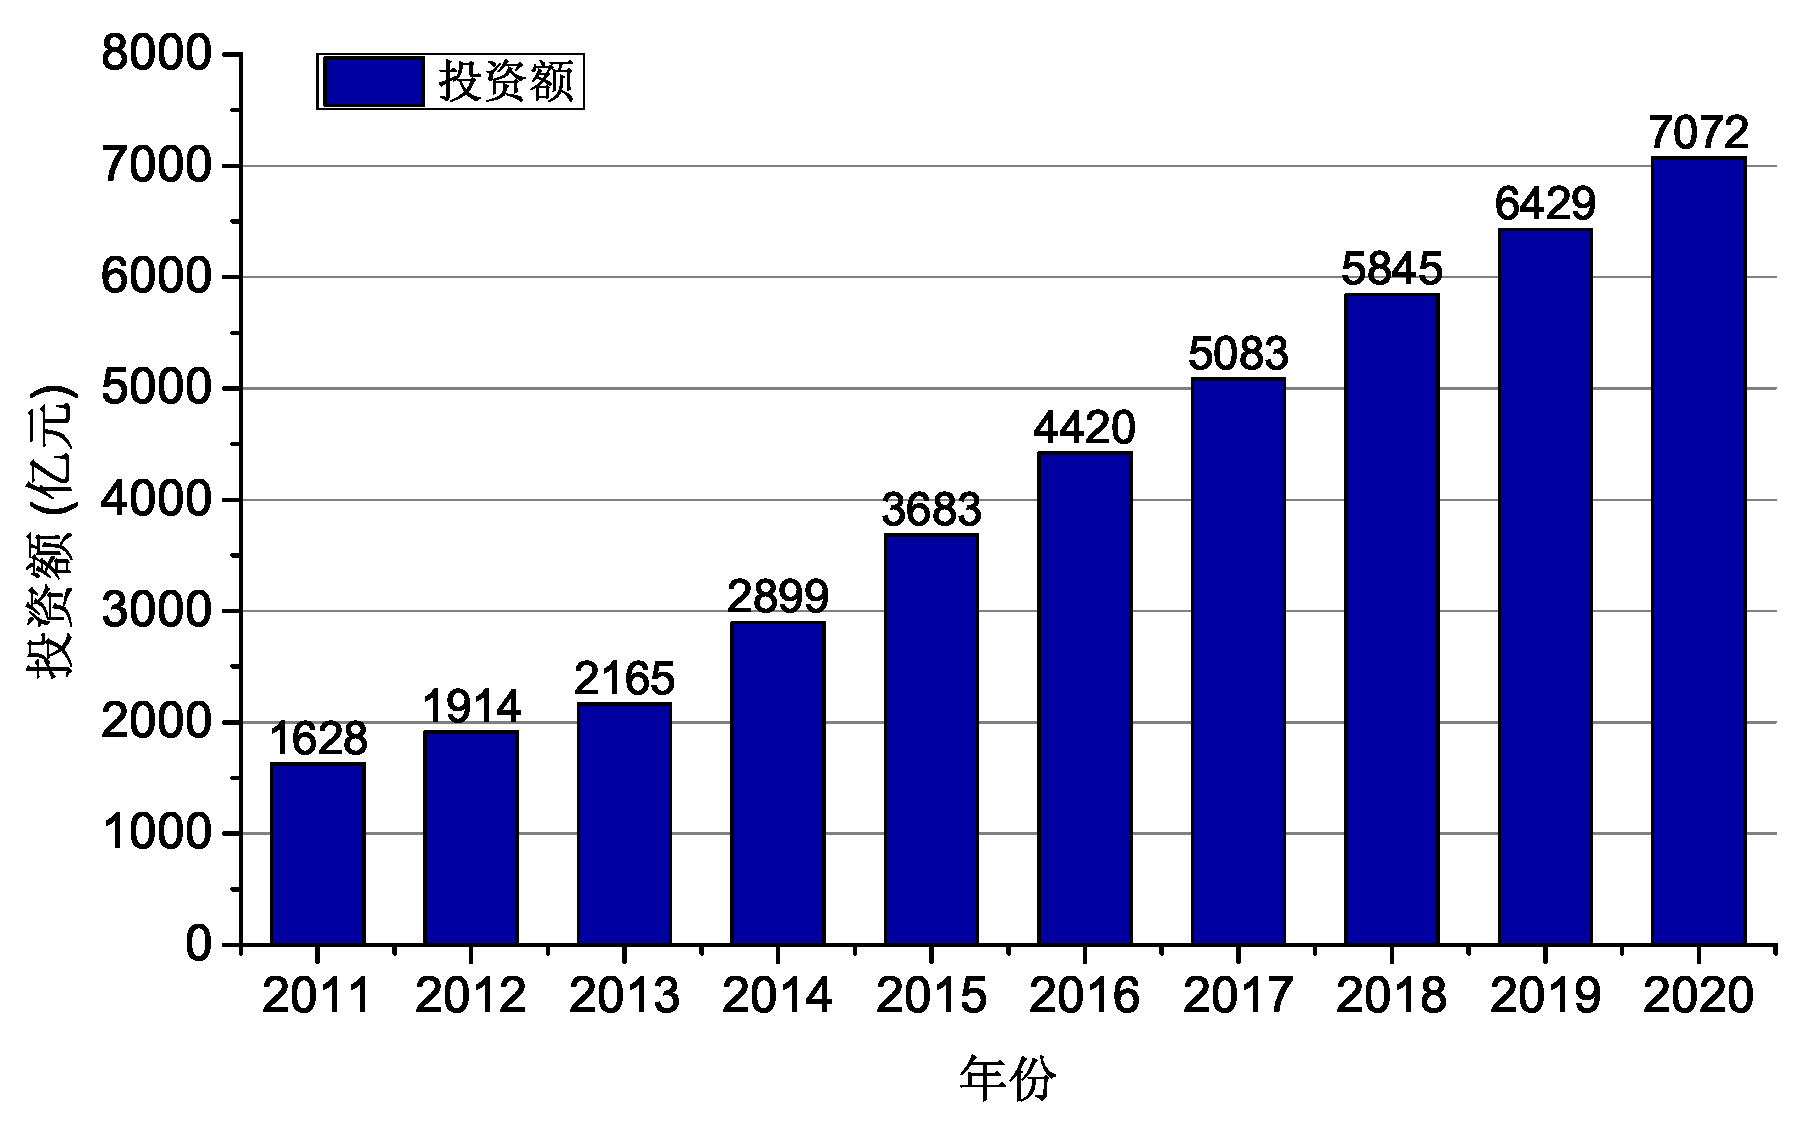
\includegraphics[width=0.7\textwidth]{chap1/investment.eps}
	\caption{中国城市轨道交通投资额}
	\label{fig:城市轨道交通投资额}
\end{figure}

我国城市轨道交通建设发展快但历史短,人们对结构健康服役问题的严重性重视程度不够。作为重大地下工程的城市轨道交通盾构隧道,所处岩土条件复杂、周边环境敏感、列车运行密度极高、使用条件苛刻,结构自身在多因素长期作用下性能不断劣化,一旦损坏不易或不可更换,并将会诱发地下工程灾害,因而对城市轨道交通盾构隧道健康服役提出了极高的要求。目前运营中的城市轨道交通健康服役问题已开始显露。

上世纪70年代建成的香港地铁部分隧道,在90年代就发现内排钢筋严重锈蚀,导致混凝土保护层的剥落,影响到正常使用。2001年5月22日,台北地铁淡水线士林站附近道床发生裂缝,地铁被迫减速,并改为手动驾驶,10万旅客上班受阻。北京地铁第一期工程1971年投入运营数年后,发现严重的杂散电流,已造成主体结构钢筋腐蚀,隧道内水管腐蚀穿孔。2006年8月19日,上海轨道交通2号线河南路-陆家嘴站越江隧道泵站由于振动与结构渗漏水的耦合叠加作用发生涌水冒浆险情,造成停运数小时。2009年12月22日,上海轨道交通1号线由于隧道结构顶部碳纤维脱落造成陕西南路至人民广场区间突发供电触网跳闸故障,造成该区列车停驶,16万人受困于地铁内、数百万人出行受阻,为建国以来城市轨道交通发生的最大事故。 

国外同样,2017年美国土木工程师协会(ASCE,\citeyear{ASCE2017})评价美国土木基础设施的平均等级为D+,估计需要花费20000亿美元才能够挽救这种长期忽视的问题。1999年10月9日,日本山阳城际新干线Kitakyushu隧道发生混凝土掉落击中电网事故,造成多趟列车取消,62000人因此出行受阻,事故调查显示原因是由于混凝土施工过程中存在缺陷,在渗漏、温度变化、列车振动等长期作用下导致裂隙不断发展所致。列宁格勒地铁1号线“森林”车站到“英勇广场”车站区间 1975 年投入运营。1994年隧道(通过钢板隔水层上的卸压排水管)经常间歇性涌水涌砂,1995年12月3日夜,下线隧道大量涌水,上线隧道急剧下沉,1995年12月4日,隧道运营终止。

上述事故表明,城市轨道交通地下结构在服役环境不断变化、材料劣化等内外因素共同作用下,其受力状态会发生变化,性能逐步退化,加之我国轨道交通建设速度迅猛,其结构施工质量难免存在一定程度的缺陷,因而城市轨道交通盾构隧道健康服役面临的问题日益突出。

综上所述,本文的研究意义体现在以下三个方面:(1)盾构隧道服役性能评估与分析有助于延长隧道的使用寿命。在隧道投入运营后,病害的出现势必缩短隧道使用寿命,适时合理的维修有助于延长隧道寿命。通过隧道结构服役性能理论研究,可以指导隧道维修时机,掌握隧道服役性能状况,制定科学的维修加固措施,延长隧道的结构劣化。

(2)盾构隧道服役性能评估与分析有助于提升城市轨道交通的社会形象。隧道作为轨道交通线路的重要一环,其健康安全是整条线路通畅运行的基础,一旦出现安全事故或列车停运,其社会负面影响将是难以估量的,严重时会影响到社会的稳定。因此全面掌握隧道服役性能状态,将安全隐患消灭在萌芽状态,保证线路的安全畅通。

(3)盾构隧道服役性能评估与分析有助于降低城市轨道交通养护维护成本。目前各国的土建结构维护费改建费增加迅速,维护费用成为财政的巨大负担。由于目前盾构隧道结构健康评估理论的不成熟,导出盲目维修、过度维修的现象,不但使得隧道病害未能得到有效治理,也造成巨大的经济浪费。因此对隧道服役性能的研究,可以以最少的资金投入达到最优的治理效果,具有重大的经济效益。

%%%%%%%%%%%%%%%%%%%%%%%%%%%%%%%%%%%%%%%%%%%%%%%%%%%%%%%%%%%%%%%%%%%
\section{国内外研究现状}
%+++++++++++++++++++++++++++++++++++++++++++++++++++++++++++++++++%
\subsection{盾构隧道服役性能评估进展}

目前隧道的服役性能评估方法大致可以分为三种:(1)基于隧道不同单项指标的劣化程度对隧道结构进行评估,在实际工作中最为常用,各国的隧道养护维护规范、手册均给出不同指标的评判标准;(2)基于历史数据建立数学模型对隧道结构进行综合性评估,如专家打分、决策树、概率论、层次分析法、模糊综合等;(3)基于数值模拟分析的评估方法,通过建立精细化数值模型,分析评估指标的评判标准。

\subsubsection{基于单项指标的评估方法}

日本《公路隧道维持管理便览》(日本公路协会,\citeyear{日本公路协会2000公路隧道维持管理便览})主要从隧道病害的发展和掉落的危险性和紧急程度来划分,根据隧道病害的严重性,从外力、材料劣化以及漏水等三个方面考虑,将评估指标划分为3A、2A、A、B四个等级,给出了衬砌变形、沉降、裂缝、剥落、漏水、湧砂、混凝土强度降低、钢筋锈蚀等指标的评判标准。

美国《公路和铁路交通隧道检查手册》(FHWA,\citeyear{FHWA2005Highway})给出隧道病害检测的一般流程,将隧道病害分为轻度、中度和严重三个等级,并规定了病害定量或者定性的评估标准。同时该手册建立了隧道结构的状态的状态分级标准,总共分为0到9十个级别,但手册只是定性地给出这十个等级的评定标准,并未给出具体的、定量的评价方法。

我国《地铁设计规范》(GB50157,\citeyear{GB501572013})对各类隧道病害指标作了规定,如建议衬砌环的直径变形控制在4-6\%衬砌直径以内;地下车站、连接通道和机电设备集中区段的防水等级应为一级,不允许渗水,结构表面无湿渍,区间隧道及连接通道等附属隧道机构防水等级应为二级,顶部不允许滴漏,其他不允许漏水,结构表面可有少量湿渍;衬砌管片的接缝张开量控制在1-2mm以内等。该规范并未对隧道状态评估进行规定。

我国《盾构法隧道结构服役性能鉴定规范》(DG/TJ08-2123-2013,\citeyear{DGTJ0821232013})根据设计规定、使用时间、使用条件和使用状况,进行结构服役性能鉴定。将隧道结构服役性能等级分级为正常、退化、劣化、恶化、危险五个等级,如表~\ref{tab:服役状态等级分级标准}~所示。将隧道结构服役状态鉴定分为五个层次,分别为隧道结构使用环境、构件服役状态等级评定、结构连接服役状态等级评定、结构区段服役状态等级评定和隧道整体服役状态等级评定,每一个层次的评定根据上一个层次评定结果所占比例决定。

\begin{table}[htbp]
  \centering
  \caption{盾构隧道服役状态等级分级标准}
    \begin{tabular}{?c"c"m{19.065em}"c?}
    \thickhline
    分级    & 服役状态  & \multicolumn{1}{c"}{分级定义} & 图示色彩 \bigstrut\\
    \thinhline
    i     & 正常    & 结构区段中的构件无安全隐患、无显著变形、无渗漏 & 绿色 \bigstrut\\
    \thinhline
    ii    & 退化    & 结构区段中部分构件耐久性退化,个别构件变形较大或结构连接处渗漏,但构件无安全隐患。 & 蓝色 \bigstrut\\
    \thinhline
    iii   & 劣化    & 结构区段中多数构件的耐久性劣化,整体变形较大或部分结构连接渗漏,但构件无安全隐患。 & 黄色 \bigstrut\\
    \thinhline
    iv    & 恶化    & 结构区段中整体变形较大 或多处结构连接明显渗漏,但无安全隐患。 & 橙色 \bigstrut\\
    \thinhline
    v     & 危险    & 结构区段中构件安全性不足、或结构区段变形过大或结构连接出现线流、漏泥沙。 & 红色 \bigstrut\\
    \thickhline
    \end{tabular}%
  \label{tab:服役状态等级分级标准}%
\end{table}%

\subsubsection{基于数学模型的评估方法}

吴江滨(\citeyear{吴江滨2004铁路运营隧道衬砌状态评估体系的建立及工程应用研究})在收集100余座铁路运营隧道数据基础上,提出隧道衬砌状态的评价体系,各个评价指标的评估标准根据应力集中系数给出,采用层次分析模型对隧道进行评估。但由于评价指标仅仅考虑了衬砌厚度和衬砌背后接触情况,评价指标过少,该评价体系未能很好反映隧道真实状态。

罗鑫(\citeyear{罗鑫2008公路隧道健康状态评估方法及系统研究})根据综合评估指标遴选原则和层次分析法原理,确定并建立了公路隧道结构健康状况综合评估体系,给出了不同评估指标的定量评定标准。采用乘积标度发确定指标的标度权重,再根据指标权重和样本数据,采用人工神经网络和模糊理论确定准则层指标权重,给出了隧道健康状态的模糊综合评价模型。

刘涛(\citeyear{刘涛2008既有盾构隧道结构性能评价研究})研究了现有城市盾构隧道的评估体系构成,和相应的评估工作流程,认为盾构隧道结构服役性能应该包含结构的安全性和耐久性,将评估指标分为整体的性能评估指标、安全性能的评估指标和耐久性的评估指标。并提出盾构隧道衬砌耐久性退化模型,基于Bayesian条件概率对耐久性模型进行修正,采用可靠度理论和Markov链方法对隧道结构的服役性能进行评价。

唐亮(\citeyear{唐亮2008隧道病害调查分析及衬砌结构的风险分析与控制研究})在分析隧道衬砌的主要破坏形式和影响结构安全性的风险因素基础上,设计了隧道风险的评价和接受准则,并根据故障树理论,建立隧道的衬砌结构故障树风险分析方法,对各种基本病害事件发生的概率,计算结构劣化的概率。在此之上,通过事件发生概率,提出可靠度理论的结构失效概率计算方法,辅以蒙特卡罗和有限元分析对隧道失效概率进行分析。

杨彤瑶等(\citeyear{杨彤瑶2013基于改进主元分析方法的隧道应变实时监测预警系统})针对隧道结构的实时监测异常数据分析,提出改进的主成分分析方法,即将原始数据流空间的变化趋势映射到对应的特征向量空间内,求解稳态特征向量,以瞬时特征向量和稳态特征向量关系,作为判据来对同步多维数据流进行异常变化诊断。在此基础上开发隧道实时监测预警系统,根据实测结果,该方法可以实时准确地反映隧道监测数据的异常变化。

李明等(\citeyear{李明2015基于功效系数法的隧道结构健康监测系统预警研究})引入功效系数法对隧道健康监测中的传感器监测数据的进行加权综合,实现监测数据的实时预警和评价。结合隧道结构健康监测系统特点,提出利用同一时刻所有传感器监测数据来确定结构预警指标体系,解决功效系数法中指标体系选取困难的问题。

Nývlt等(\citeyear{N2011Probabilistic})借鉴航天航空行业的风险分析概念,提出适合在隧道工程领域的风险分析方法,并结合决策树、可靠度理论、最优化方程等方法,建立满足安全风险级别下的成本最优化计算方法,该方法在实际工程应用中能指导养护维护决策,图~\ref{fig:隧道风险评估决策树}~为盾构隧道风险评估的决策树图。

\begin{figure}[!h]
	\centering
	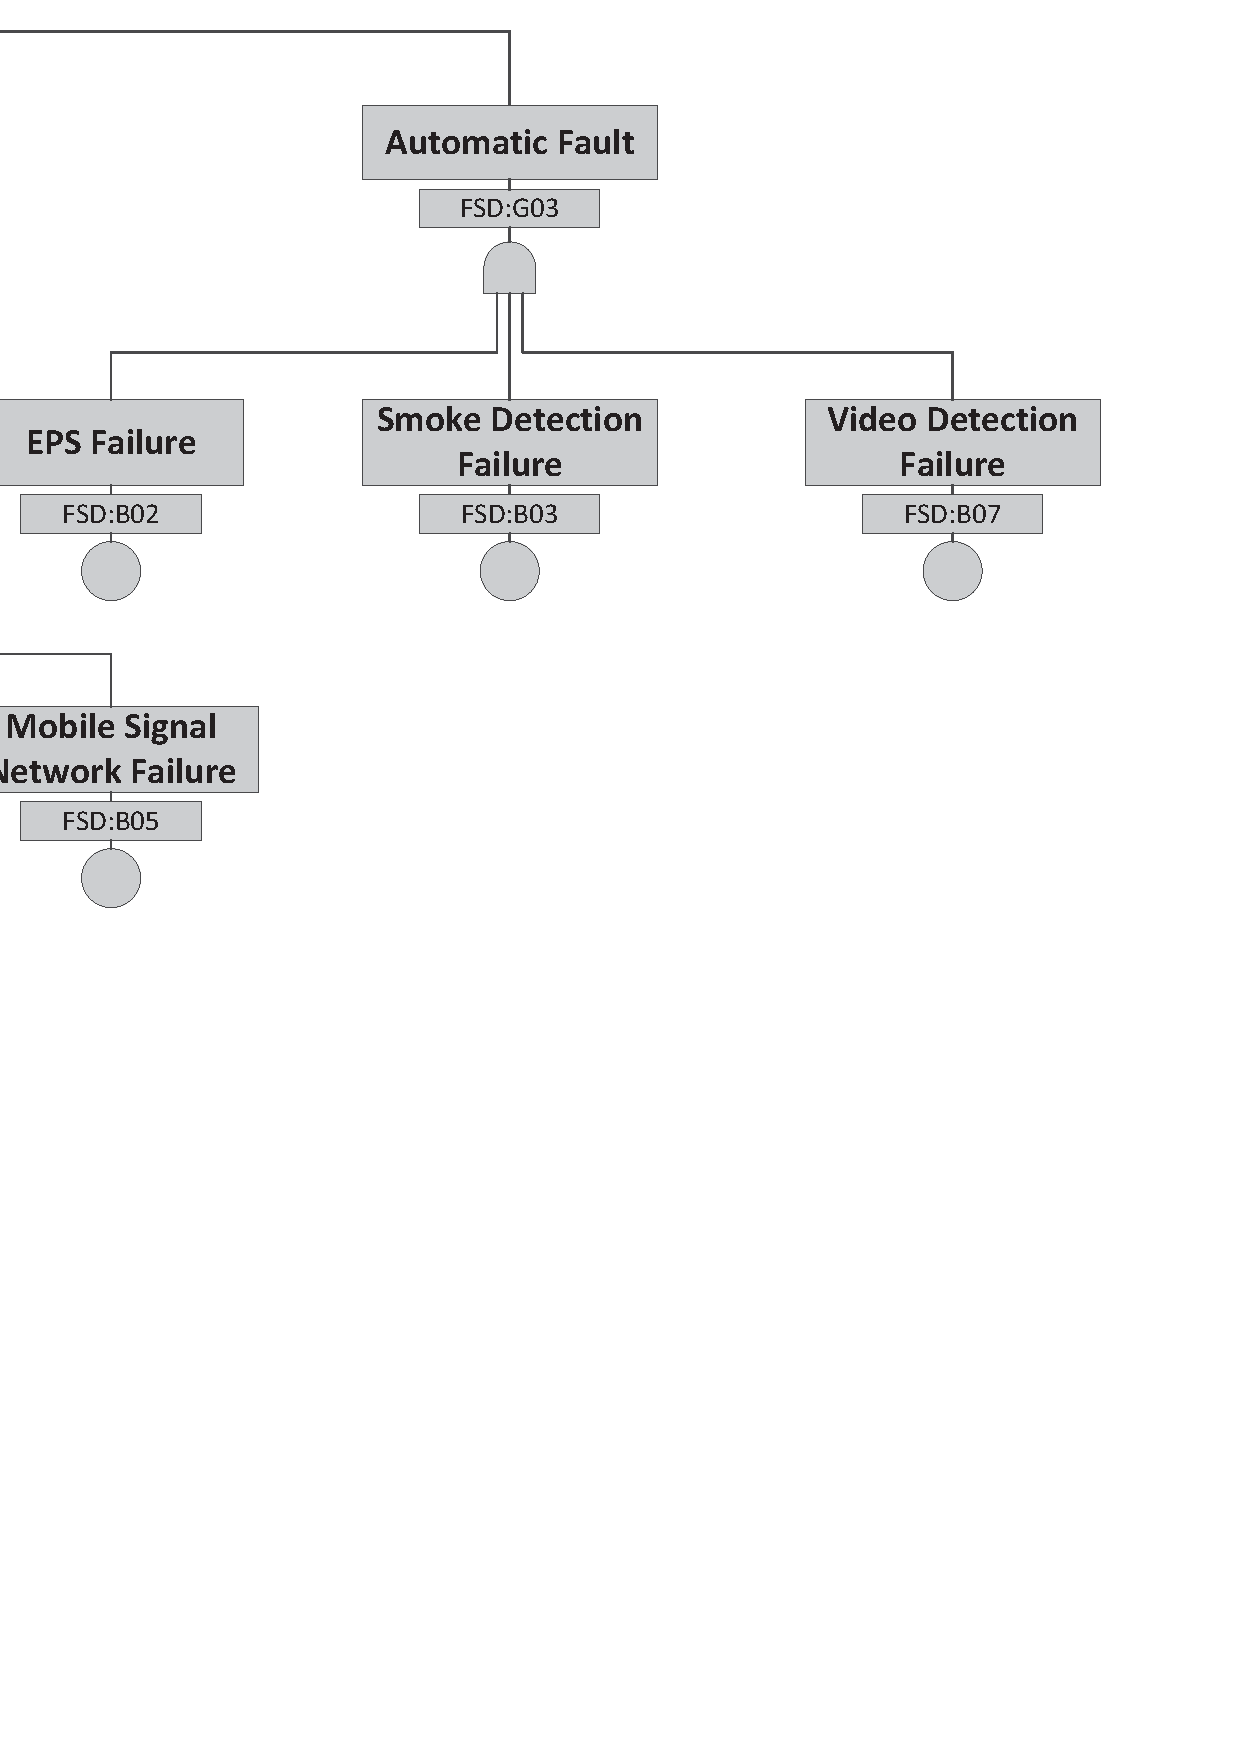
\includegraphics[width=1.0\textwidth]{chap1/nyvlt-faulttree.pdf}
	\caption{隧道风险评估决策树}
	\label{fig:隧道风险评估决策树}
\end{figure}

Yuan等(\citeyear{Yuan2012Assessment})为了量化隧道衬砌的结构性能,根据极限状态设计将其分为正常、退化、劣化、恶化、危险五个级别。结构的服役状态包括运营状态和结构状态。其中,运行状态指隧道所处环境条件环境恶劣程度。结构状态指标包括外观性、密封性、完整性、刚性和稳定性。提出了隧道结构服役状态评估的框架,依据运行状态指标和结构指标值与标准值的比较得出其所处的服役状态级别。

Zhang等(\citeyear{Zhang2014Fuzzy})采用模糊分析层次和综合评估模型,合并多个传感器的不同类型的数据,将其映射为盾构隧道的健康评分。选择分段隶属函数,并引入指数量表表征不同权重集。定义模糊运算符号,用于监测因子的模糊综合评估指标。

\subsubsection{基于力学模型的评估方法}

Cavalaro等(\citeyear{Cavalaro2011Structural})研究了施工期盾构隧道衬砌裂缝形成的主要机理,最常见的裂缝是由衬砌之间接触不均匀导致支撑受力不一致而产生的。通过建立不同的有限元模型并对比其分析结果,得出衬砌的接触不均匀直接影响了衬砌的极限承载力。

Naggar和Hinchberger(\citeyear{Naggar2012Approximate})采用数值分析方法,模拟完好的和劣化后的混凝土衬砌力学特性。使用非线性有限元模型模拟混凝土退化,并考虑了土体和混凝土的相互作用和非线性应力应变响应,用于评估劣化后的隧道衬砌的性能状态。

Li等(\citeyear{Li2015Experimental})研究了不同轴向应力水平下弯矩的纵向接缝张开的发展情况和极限状态中的纵向接缝张开,提出了一种渐进模型来预测接缝的力学行为。基于此模型,研究轴向应力水平,螺栓预紧力,混凝土分层深度和螺栓腐蚀深度对接缝力学性能的影响。

Li等(\citeyear{Li2015A})提出了纵缝接头张开的计算模型。模型包含接缝张开不同阶段的不同受力模式,考虑混凝土、螺栓和密封垫对张开量的影响。实验观测与计算分析得出纵缝张开过程可分为四个阶段:阶段一是一开始接缝未张开时,接头处混凝土全截面受压;阶段二接头处混凝土开始出现张开,螺栓拉力逐渐增大;阶段三为外侧边混凝土开始接触;阶段四则是螺栓屈服阶段,如图~\ref{fig:接缝张开与弯矩}~所示,此模型可用于指导盾构隧道衬砌的接缝张开评估。

\begin{figure}[!h]
	\centering
	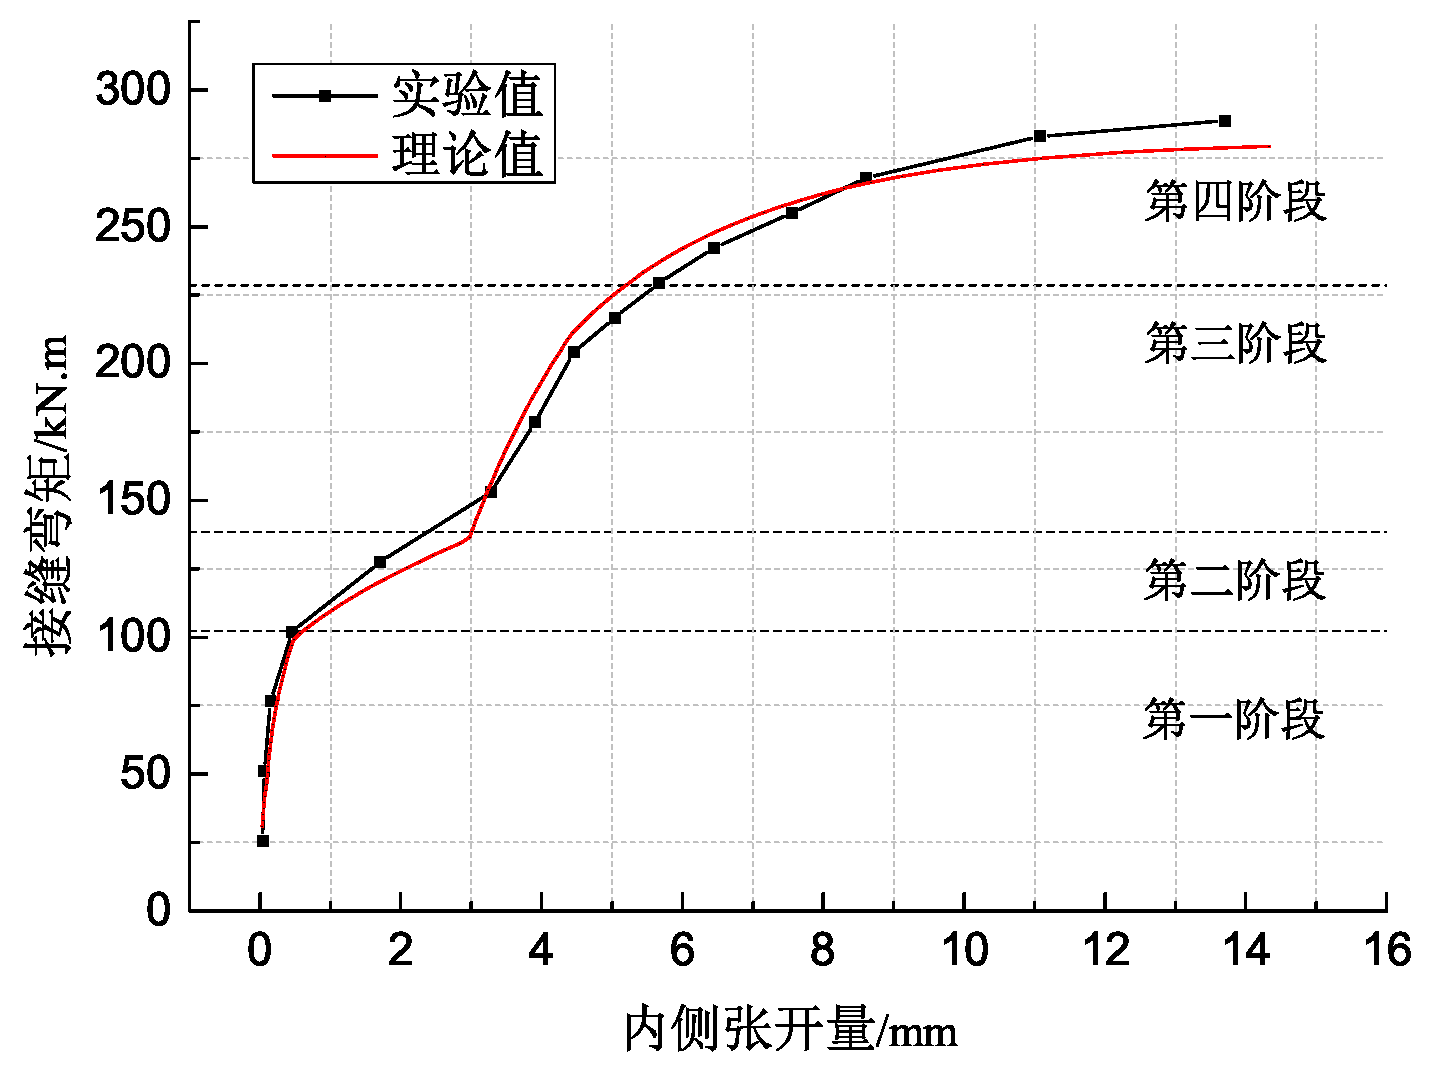
\includegraphics[width=0.7\textwidth]{chap1/joint-moment.eps}
	\caption{盾构隧道衬砌弯矩-接缝张开关系图}
	\label{fig:接缝张开与弯矩}
\end{figure}

袁勇等(\citeyear{袁勇2006运营越江隧道服役现状调查与检测评估})指出对于直径10~m的盾构隧道,隧道的纵向变形曲率半径小于40~km时,容易导致衬砌环向接头张开增大,引起渗漏。同时渗漏又导致隧道继续产生纵向不均匀变形,二者相互影响。并提出用于既有隧道结构损伤评估的宏观安全性模型和微观耐久性模型。

季倩倩(\citeyear{季倩倩2009带裂缝的盾构隧道衬砌力学模型研究})在盾构隧道的梁-弹簧计算模型中,采用弹簧单元模拟裂缝对衬砌结构的影响,建立了带裂缝的盾构隧道衬砌力学模型。分析结果指出裂缝的存在降低了衬砌的刚度,且降低程度与裂缝宽度和深度相关。

刘曙光(\citeyear{刘曙光2012盾构隧道混凝土管片的承载力退化模型})在现有钢筋混凝土正截面承载力计算方法基础上,考虑了锈蚀钢筋混凝土受弯构件的正截面承载力计算方法,提出盾构隧道衬砌的承载能力退化模型,模型有水平段的诱导期和下降段的劣化期组成,可用于盾构隧道混凝土管片的寿命评估。

王如路和张冬梅(\citeyear{王如路2013超载作用下软土盾构隧道横向变形机理及控制指标研究})采用数值模拟方法分析地面压载、土体侧向压力、土体抗力对盾构隧道收敛变形的影响,给出了收敛变形随压载的变化规律,得出收敛变形与衬砌受力、螺栓受力和接缝张开量的关系曲线,在实际工程中可根据隧道的直径测量量判断隧道的变形状态,为隧道的安全性评价提供指导。

丁文其等(\citeyear{丁文其2013基于地层})采用地层-结构法研究隧道初始地应力平衡、施工顺序、材料本构模型和接触关系等问题,分析不同因素对隧道沉降变形和接头相对变形的影响。

%+++++++++++++++++++++++++++++++++++++++++++++++++++++++++++++++++%
\subsection{盾构隧道服役性能预测进展}

针对盾构隧道结构出现的病害,现有的计算方法还很难全面模拟材料的真实特性、结构与环境的真实状态,因而难以准确评价结构服役性能和确定病害成因、发展趋势及其对服役性能的影响。目前主要有两类方法对盾构隧道服役性能进行预测:(1)考虑材料性能退化的影响,结合盾构隧道数值模型,分析服役性能的退化;(2)基于历史数据,建立数学模型,采用大量数据对模型参数进行估计训练。

\subsubsection{基于材料劣化的性能预测}

Marchand等(\citeyear{Marchand2002Theoretical})研究了弱硫酸根离子对混凝土耐久性的影响,分别试验了水灰比为0.45、0.65、0.75,CSA10和50类型水泥,硫酸盐浓度0-30~mmol/l的不同方案,得出混凝土在硫酸根离子溶液中的退化规律。

Liu等(\citeyear{Liu2014A})考虑早龄期混凝土各组分材料随机分布的影响,及由于水化反应造成的热力学性能时变性和体积变形,将宏观尺度划分为混凝土、砂浆、水泥浆三个不同尺度,对混凝土早龄期性能进行跨尺度研究。建立非线性粘弹性早龄期混凝土多尺度本构模型,并与时间耦合的本构关系。

李忠等(\citeyear{李忠2009氯离子侵蚀盾构隧道衬砌结构性能退化试验})对盾构隧道衬砌钢筋进行加速锈蚀实验,得到不同锈蚀程度的钢筋构件,再对锈蚀钢筋的承载力、变形和破坏特征等作相关测试,获取隧道衬砌结构在氯离子侵蚀下的性能退化规律。

张红光等(\citeyear{张红光2014开裂混凝土内氯离子扩散机理及数值模拟研究})研究得出混凝土结构在初始损伤和裂缝存在情况下,容易造成氯离子等侵蚀性介质在混凝土中快速扩散,通过实验观察和数值模拟,归纳氯离子在混凝土中的扩散系数表达式,为评价混凝土结构的耐久性提供依据。

\subsubsection{基于数学模型的性能预测}

在工程领域,退化模型包括马尔科夫链模型(Madanat等,\citeyear{Madanat1997Probabilistic})、时间序列模型(Prozzi,\citeyear{prozzi2001modeling})、泊松回归模型(Ching和Leu,\citeyear{ching2009bayesian})、灰色预测模型(Wang和Li,\citeyear{wang2011pavement})等,其中马尔科夫链和时间序列最为常用。

Carnahan等(\citeyear{camahan1987optimal})提出马尔科夫链是一种时间离散基于状态的退化模型,其基本假定包括:1)有限个状态;2)状态转移概率只依赖当前的状态;3)转移概率矩阵与时间无关。马尔科夫链模型的转移概率可通过期望值法来估计,但期望值法无法显式地表示影响因素对于状态的影响、考虑退化过程与时间的依赖性、表示连续的退化过程。

Madanat等(\citeyear{Madanat1997Probabilistic})分别采用了泊松回归模型、有序概率模型来估计马尔科夫链模型中的转移概率矩阵,解决了期望值法无法显式地表示影响因素对于状态的影响、考虑退化过程与时间的依赖性、表示连续的退化过程的问题,可以考虑导致状态变化的影响因素和时间因素。

DeStefano和Grivas(\citeyear{destefano1998method})提出了基于时间的模型以计算状态转移概率。Mishalani和Madanat(\citeyear{mishalani2002computation})提出了基于时间状态离散的随机持续时间模型,能够考虑时间、状态之间的依赖性,表征退化过程与影响因素之间的关系,并且用钢筋混凝土桥面板实例阐述了该方法的可行性。

Chu等(\citeyear{chu2005estimation})提出结构化时间序列模型,该模型可以解释采用不同数据采集方式获取的数据之间的不确定性,同时该模型也可辅助得出维护养护决策时的最优化方案,可以替代传统的马尔科夫链模型。

Chu等(\citeyear{chu2007estimation})采用自回归滑动平均时间序列模型(ARMA 模型)预估基础设施的性能变化,其能考虑状态空间的相互依赖性,预测样本空间外结构的性能变化趋势,也可作为马尔科夫链模型的一种替代方法。

曹净等(\citeyear{曹净2014基于})提出基于小波变换和粒子群优化的最小二乘支持向量机,结合自回归移动平均模型,预测基坑变形的时间序列数据。基于小波变化先将时间序列数据分解为趋势时间序列和随机时间序列两个子序列,分别采用支持向量机和自回归移动平均模型来预测两个子序列,最后再相叠加得到最终预测结果。

文明等(\citeyear{文明2015地铁车站施工过程中地表沉降的})针对时间序列模型的单一线性和忽略外部因素影响的问题,建立了非线性自回归神经网络时间序列模型,如图~\ref{fig:非线性自回归神经网络}~所示,该模型具有延迟单元和反馈结构,并且可以将外部因素作为外部输入,预测结果适应性更好、准确性更高。

\begin{figure}[!h]
	\centering
	\includegraphics[width=0.9\textwidth]{chap1/NARXNN.pdf}
	\caption{非线性自回归神经网络时间序列模型(文明等,\citeyear{文明2015地铁车站施工过程中地表沉降的})}
	\label{fig:非线性自回归神经网络}
\end{figure}

%+++++++++++++++++++++++++++++++++++++++++++++++++++++++++++++++++%
\subsection{盾构隧道服役性能服务进展}
\label{chap:service-intro}

随着信息技术的不断发展,数字化技术成为改革传统模式的重要手段,高效的盾构隧道服役性能评估与预测服务同样需借助数字化技术。在土木工程领域,常用的数字化技术包括三大类:(1)地理信息系统(GIS);(2)建筑信息模型系统(BIM);(3)综合性的智慧服务系统。

\subsubsection{基于地理信息系统的服务平台}

地理信息系统(Geographic Information System,GIS)是一门结合地理学、地图学、遥感、计算机等的综合性学科,目前在不同的领域得到广泛应用,主要用于输入、存储、查询、显示和分析地理数据的系统。早期在地下工程主要用于地质数据的存储,如Rosenbaum和Warren(\citeyear{rosenbaum1986creating})早在1972年就为伦敦的地质钻孔数据建立了地理数据库,可用于地下公路、铁路开挖时的周边环境评估。

Baffour和Abatan(\citeyear{baffour2002developing})结合探地雷达(GPR)、全球定位系统(GPS)和地理信息系统,开发了地下基础设施的数字化采集、处理、管理信息系统,该系统具备空间信息和属性信息的管理能力,为地下基础设施提供定位、分析等高效的功能。

Chang和Park(\citeyear{chang2004development})基于Web技术开发了钻孔数据和地层数据的GIS管理系统,在系统建立在钻孔和地层的数据标准和数据库标准之上,合计存储了超过10000个钻孔和首尔地层等数据,用户通过互联网可以方便地对这些数据进行检索、统计分析。

近年GIS的地理数据分析功能逐渐被重视,如Yoo和Kim(\citeyear{yoo2007tunneling})首先用人工神经网络(ANNs)预测一般隧道设计中的隧道性能预测,对于隧道工程现场,经校正有限元模型改进过的ANNs能根据稳定性和附近环境的影响得出隧道环境和性能的关系。并把ANNs植入到GIS,利用GIS的数据管理和可视化功能进行分析,如图~\ref{fig:集成GIS和ANN的隧道掘进性能概念}~所示,该平台的最大优势是加快了隧道性能的评估,从而缩短隧道设计的时间。

\begin{figure}[!h]
	\centering
	\includegraphics[width=0.9\textwidth]{chap1/ann-gis.png}
	\caption{集成GIS和ANN的隧道掘进性能概念(Yoo和Kim,\citeyear{yoo2007tunneling})}
	\label{fig:集成GIS和ANN的隧道掘进性能概念}
\end{figure}

Yuan等(\citeyear{yuan2012study})基于GIS数据管理,在GIS系统中实现了隧道开发对岩体变形和地表建筑物影响的分析功能,并建立数值模型分析由于开挖变形引起的地表建筑物的应力-应变关系曲线,该平台为隧道施工期间的防灾减灾提供了快速的评估依据。

Li和Zhu(\citeyear{li2013development})开发轨道交通数字化平台,以满足盾构隧道施工运营过程中数据管理、数据分析和可视化要求。根据已有工程数据标准,结合以往盾构隧道工程实例,提出轨道交通地下结构全生命周期数据标准和数据库设计,主要分为地质、结构和监测三部分。利用Web-GIS软件和Web Service技术开发基于互联网的数字化平台。

解福奇等(\citeyear{解福奇2009时态})建立了考虑时间的多维、动态GIS模型,可在该模型上对时态数据进行操作和处理,能实时反映时态数据属性的变化,且模型也提供了方便的数据库查询和检索功能,采用三维可视化技术将模型运用于隧道工程的数字化施工当中。

刘振平等(\citeyear{刘振平20173d})采用GRASS GIS、Python等建立了GIS和有限元模拟分析的开发框架,实现了网格剖分算法,改良3D GIS中的TIM模型,使其适合有限元模拟的地质切面的三角形网格,结合GIS的空间分析功能,得到GIS与有限元分析无缝结合的隧道地表沉降规律分析功能。

\subsubsection{基于建筑信息模型的服务平台}

建筑信息模型(Building Information Model,BIM)是以建筑工程项目的各类信息数据作为基础,建立三维建筑模型,通过数字仿真技术模拟建筑物所具有的所有真实信息。统一的建筑信息模型能让业主单位、设计单元、施工单位和监理单位等多个项目参与方,共享同一模型。目前BIM在土木工程中的应用包括三维可视化、成本造价、几何碰撞、施工仿真、能耗分析、养护维护等。

Motamedi和Hammad(\citeyear{motamedi2009lifecycle})认为BIM将成为工程全寿命周期中创建、共享、交换和管理信息的方法,当前RFID技术已经成为成熟的数据自动采集和信息存储技术,该技术可为BIM收集各类全寿命数据作为基础数据,讨论了BIM系统数据的存储和检索设计。

Zhang等(\citeyear{zhang2013building})将自动化安全规则检查集成在BIM模型中,开发了不同情况下的算法程序,可自动分析建筑模型和监测安全隐患,向用户建议预防措施。该系统可用于设计期的自动化危险识别和纠正,预防在施工期发生安全事故。

李德超和张瑞芝(\citeyear{李德超2012bim})将数字城市模型与BIM模型集成一体。数字城市模型主要利用GIS技术,以城市地理空间数据为基础,建立的城市数字信息模型,集成BIM可实现城市数字模型的资源共享,以及多领域对城市模型的协同作业。

于金勇和林敏(\citeyear{于金勇2013bim})将地铁设计电子图纸转换成BIM建筑、结构、机电模型,并整合在一起,利用BIM软件的碰撞分析得出碰撞点,对BIM模型进行重新设计消除碰撞点,优化了地铁安装工程的施工方案,避免了工程在验收阶段的返工误工现象出现。

王慧琛等(\citeyear{王慧琛2013bim})将BIM技术应用于地铁车站的设计期和施工期两个阶段,应用主要包括两个方面,一方面采用BIM技术对地铁车站工程建立全专业设施模型,分析各专业设备之间碰撞。另一方面也利用BIM模型对整体工程进行虚拟仿真及4D施工模拟。

BIM技术在应用过程中有三方面的挑战,包括标准层面、技术层面和管理层面,在BIM技术标准层面,最重要的内容即是建筑信息的数据交换标准。IFC(Industry Foundation Class)标准是国际通过的BIM数据标准,现有的IFC版本已经可以较好描述建筑工程的全寿命周期信息,对于地下基础设施领域的研究也已取得部分成果。

如Yabuki(\citeyear{yabuki2013development})在IFC标准基础上提出并改进了盾构隧道的数据模型IFC-ShieldTunnel。该数据模型在IFC框架内增加了盾构隧道特有的对象实体,如管片、防水材料等,并通过实际工程验证了模型的适用性。该研究团队还计划对该数据模型在盾构隧道施工进度和成本造价方面的扩展研究。IFC-ShieldTunnel基本确定了盾构隧道全寿命周期数据模型的框架体系。

Borrmann和Jubierre(\citeyear{borrmann2013multi})认为现有的IFC标准无法从多个详细程度对大型基础设施的信息进行描述,因此在Yabuki的盾构隧道信息模型基础上引入LoD和Refines实体,不同详细程度的信息对象进行定义。同时,为保持不同LoD间几何信息的连贯性,对不同LoD中几何对象的引用关系进行了研究。 

林浩(\citeyear{林浩2016基于})认为IFC-ShieldTunnel信息模型中定义的部分实体只是停留在语义状态,此外,在地质信息领域,IFC-ShieldTunnel 没有描述土工试验信息;在施工信息、监测信息和结构病害信息领域,IFC-ShieldTunnel也未见相关资料信息;故对IFC-ShieldTunnel进行扩展。

\subsubsection{综合性的智慧服务平台}

目前GIS和BIM系统应用于地下工程仍存在许多问题,如GIS对非地理数据只能将其作为地理数据的属性数据进行管理,而且GIS本身并没有规定数据标准,而是由用户自行定义,导致不同用户之间数据共享困难。BIM最初是针对地面建筑提出,逐渐扩展至土木工程的不同领域,但BIM没有提出完整的信息流概念,只是停留在对信息模型本身的管理,造成信息流通不通畅的问题。基于上述原因,许多学者提出开发了综合性的智慧服务平台。

朱合华和李晓军(\citeyear{朱合华2007数字地下空间与工程})系统提出了数字地下空间与工程的基本概念,其应提供开放的信息组织方法与信息发布机制,建立健全的数据标准与数据处理的方法,具备可视化手段。综合性的数字化地下空间与工程可以实现信息发布与共享,并对海量的工程数据进行动态管理,提供不同的数据可视化方式,从而提高工程管理效率。

李晓军等(\citeyear{李晓军2009盾构隧道数字化研究与应用})提出盾构隧道的数字化概念,即让复杂多变的地下工程变得更加透明,对工程全寿命周期数据的管理,最终辅助工程分析与智能决策。该系统采用客户端-服务器架构,将工程数据分为空间信息数据和属性信息数据两种,并对三维隧道和三维地层进行建模,实现工程可视化。

朱合华等(\citeyear{朱合华2015基础设施建养一体数字化技术})提出基础设施的建养一体数字化的概念,从基础设施建设和养护一体的角度考虑,结合工程、经济和管理的手段,以最优方式保障基础设施工程的安全。建养一体化的数字平台包括了数据采集、处理、表达、分析等功能,集成了采集技术、数据标准、可视化建模、空间分析和数字数值一体化分析等技术。

自从2008年IBM公司提出“智慧地球”的概念(IBM,\citeyear{IBM2008Wisdom}),“智慧化”一词成为新的研究热点。在土木领域,“智慧城市”的概念随之形成(巫细波和杨再高,\citeyear{巫细波2010智慧城市理念与未来城市发展}),结合物联网、云计算和大数据等信息技术,对城市中的基础设施赋予接入网络的能力,通过网络将城市基础设施联系在一起。智慧城市并不是单一技术的累加,而是“数字城市+物联网+云计算+大数据”(李德仁等,\citeyear{李德仁2013智慧城市的概念})。

英国剑桥大学于2011年成立智慧基础设施研究中心(Cambridge Centre for Smart Infrastructure and Construction,CSIC),此研究为响应英国政府颁发的英国基础设施建设计划(Treasury,\citeyear{treasury2011national}),收集掌握英国所有基础设施当前状态、制定合适的养护维护措施、降低维护成本和延长基础设施的使用寿命。CSIC(\citeyear{CSIC2011Cambridge})采用了无线传感器等监测手段,实现对基础设施的可持续发展的目标。

朱合华等(\citeyear{朱合华2018智慧基础设施})于2013年提出基础设施智慧服务系统(infrastructure Smart Service System,iS3)的概念,从信息流的角度,实现基础设施的智慧化管理。iS3系统包括数据的采集、处理、表达、分析和服务决策等五个方面,如图~\ref{fig:iS3概念图}~所示,并兼容GIS系统与BIM系统。

\begin{figure}[!h]
	\centering
	\includegraphics[width=1.0\textwidth]{chap1/iS3.pdf}
	\caption{基础设施智慧服务系统(iS3)概念图(朱合华等,\citeyear{朱合华2018智慧基础设施})}
	\label{fig:iS3概念图}
\end{figure}

%%%%%%%%%%%%%%%%%%%%%%%%%%%%%%%%%%%%%%%%%%%%%%%%%%%%%%%%%%%%%%%%%%%
\section{目前研究存在的问题}

%+++++++++++++++++++++++++++++++++++++++++++++++++++++++++++++++++%
\subsection{服役性能评估的问题}

已有基于单项指标的评估方法未能对盾构隧道的整体服役性能作出评判,而且同一段隧道采用不同的单项指标评估将得到不同的评估结果。目前根据调查研究,盾构隧道在运营期会出现许多病害,如衬砌缺角、掉块、混凝土碳化、剥落、剥离、空洞、钢筋锈蚀、空气水环境中的氯离子、硫酸根离子等(Yuan等,\citeyear{yuan2013predictive})。叶耀东等(\citeyear{叶耀东2007软土地铁运营隧道病害现状及成因分析})总结了上海地铁盾构隧道在运营期的主要病害有渗漏水、裂缝、损坏、纵向沉降和收敛变形等。对于这么多单项病害,现有的单项指标评估方法未对所有的单项指标给出评判标准。不过这种方法因为使用简单,在实际工程应用较多,并编写成行业规范。

已有基于力学模型的评估方法较难建立考虑真实病害情况的数值模型,而且即使有能建立相应的数值模型,其计算分析时间较长。如考虑衬砌纵缝接头的力学性能,建立三维精细化接头力学模型,张厚美等(\citeyear{张厚美2000圆形隧道装配式衬砌接头刚度模型研究})构建的三维有限元模型中,混凝土采用实体单元和弹塑性本构,衬垫采用板单元和曲线本构,连接螺栓采用杆单元,衬垫与混凝土表面之间设置接触单元;曾东洋等(\citeyear{曾东洋2005地铁盾构隧道管片接头刚度影响因素研究})引入面-面接触单元和衬垫单元模拟各构件之间的接触关系;Chen等(\citeyear{chen2009numerical})接头三维精细化有限元模型包括管片、接头、螺栓及手孔等,分析了施工期和服役期盾构隧道管片裂缝或破损问题。虽然上述模型能较好地分析隧道服役性能劣化的原因,但在评估分析过程中比较耗时。

已有基于数学模型的评估方法未考虑各指标之间的相关性和单个指标权重随着指标劣化而变化的情况。在隧道服役性能评估方面,层次分析法因具有综合性强,原理简单等优点,被广泛应用(戴胜,\citeyear{戴胜2008越江盾构隧道耐久性分析与评估体系研究};李晓英等,\citeyear{李晓英2008铁路隧道健康状态模糊评价体系研究};段怀志,\citeyear{段怀志2009隧道及地下工程健康评估研究};张素磊,\citeyear{张素磊2012隧道衬砌结构健康诊断及技术状况评定研究};Rao等,\citeyear{rao2016fuzzy})。根据层次分析法的理论原理(Saaty和Vargas,\citeyear{saaty2012models}),评估指标之间是相互独立的,但实际情况并非如此,如隧道的横向收敛会导致衬砌纵缝的张开量,隧道的纵向变形会导致衬砌环向接缝的张开量和衬砌环错台的发生。另外,由层次分析法评判矩阵计算得出的指标权重是常量,在实际情况中,当某一评估指标劣化严重时,根据“木桶效应”,隧道的整体服役性能应该是迅速下降的,体现为劣化指标权重的增加。

在其他工程领域,已由点状和线状的评估方法向网格化空间评估发展,如洪水灾害评估模型基于空间网格计算洪水灾害损失(Su等,\citeyear{su2005grid});Islam等,\citeyear{islam2007grid};朱强等,\citeyear{朱强2007基于网格的洪水损失计算模型})、铁路轨道网格(或部件)的空间风险评估模型(郭孟欣等,\citeyear{郭孟欣2016基于网格的铁路建设工程风险指数评价模型研究};白磊,\citeyear{白磊2017铁路轨道健康管理网格化分析决策模型研究})、道路工程的网状路面开裂评估模型(Jenelius,\citeyear{jenelius2012road})等,对于盾构隧道相关研究较少。

%+++++++++++++++++++++++++++++++++++++++++++++++++++++++++++++++++%
\subsection{服役性能预测的问题}

盾构隧道服役性能预测缺少既能考虑时间变化趋势,又能考虑数据地理空间关系的预测方法。一般地采用数值模拟结合现场监测数据分析计算盾构隧道的评估指标大小(李喆和张子新,\citeyear{李喆2005相邻隧道施工对上海地铁二号线的影响分析};王如路,\citeyear{王如路2009上海软土地铁隧道变形影响因素及变形特征分析}),大多未研究指标随时间的变化趋势。对于考虑时间因素的数学模型,如马尔科夫链模型(Tran等,\citeyear{tran2008prediction};Abaza和Murad,\citeyear{abaza2009predicting})、时间序列模型(刘燕萍等,\citeyear{刘燕萍2010时间序列分析在建筑物变形监测中的应用};卢宏彬,\citeyear{卢宏彬2016基于时间序列的结构损伤概率方法研究})、BP人工神经网络(Tsuda等,\citeyear{tsuda2006estimating};Mahdevari和Torabi,\citeyear{mahdevari2012prediction})等,均能通过历史数据预测未来某个时间状态的值,但是上述模型只能对同一组数据进行预测,不能考虑空间上临近的数据对该组数据的影响。

%+++++++++++++++++++++++++++++++++++++++++++++++++++++++++++++++++%
\subsection{服役性能服务的问题}

基于地理信息系统的服务平台缺乏对非地理数据的有效管理和用于数据交换、共享、描述工程结构的统一数据标准。GIS系统更像是一个地理数据库的管理系统,且具备十分成熟的拓扑结构,能存储和分析大部分的空间关系,提供了基于矢量和栅格两种方式的空间分析,如图形相交、合并、最短路径、网格计算、面积计算等。

基于建筑信息模型的服务平台缺乏数据信息流管理和开发复杂分析功能的能力。BIM系统注重工程本身在设计、建设时对工程的形状、大小、空间、属性等信息的管理,且提供了便捷、简单的分析功能,如布尔运算、三维造型、碰撞分析、长度面积测量和体积计算等。但是BIM系统的所有功能均需围绕BIM模型展开,对数据全寿命期的数据流动有一定约束,另外BIM采用的直角坐标系统,没有世界地理坐标系统和拓扑结构,在BIM系统中定制复杂的分析功能困难。

考虑上述原因,近些年综合性的智慧服务平台逐渐成为发展趋势,以朱合华等(\citeyear{朱合华2018智慧基础设施})提出的基础设施智慧服务系统(iS3)为例,其从实际工程信息流角度考虑,为服务系统抽象了管理模型、数据模型和分析模型,同时借鉴GIS和BIM系统的数据存储、管理和分析功能,为工程数据和图形引擎提供开放式的接口,实现各类分析和智慧决策的服务,如图~\ref{fig:iS3-gis-bim}~所示。

目前此类综合性平台基本采用单体式应用的方式进行开发,尽管其在开发过程中是模块化的逻辑,但最终会被发布成单个应用,如C++、C\#的EXE格式,Java的WAR格式,这种方式有很大的局限性,随着时间推移,应用会越来越庞大,越难理解,不利于持续性开发,另外单体式应用某个模块的一个问题有可能导致整个系统奔溃。故现有的服务平台缺少一种低耦合、高可靠、易扩展的服务框架。

\begin{figure}[!h]
	\centering
	\includegraphics[width=0.9\textwidth]{chap1/iS3-gis-bim.pdf}
	\caption{iS3 与 BIM, GIS 的区别与联系}
	\label{fig:iS3-gis-bim}
\end{figure}

%%%%%%%%%%%%%%%%%%%%%%%%%%%%%%%%%%%%%%%%%%%%%%%%%%%%%%%%%%%%%%%%%%%
\section{论文研究内容、路线和创新点}

%+++++++++++++++++++++++++++++++++++++++++++++++++++++++++++++++++%
\subsection{主要研究内容}

本文以上海运营地铁盾构隧道为研究对象,研究如何根据已有的监测检测数据,客观定量地评估盾构隧道当前服役性能,且在大量历史数据基础上,对未来某个时间盾构隧道的服役性能作出预测,以及探讨了服役性能评估与预测方法在实际工程中的服务机制。各章节的主要研究内容如下:

第二章参考美国国家公路协会对路面服役性能评估方法,对盾构隧道进行病
害数据采集,专家打分,和打分结果的回归拟合,得出适合盾构隧道的服役性能指标,建立服役性能指标与相对沉降平均值${sett}_{a}$、平均差异沉降$set{{t}_{d\_a}}$、平均收敛变形率${cov}_{a}$、百环渗漏水面积${d}_{l}$、百环衬砌剥落面积${d}_{s}$、百环裂缝长度${d}_{c}$的定量公式,并采用变权理论对公式进行全寿命期的修正。

第三章研究了适用于盾构隧道沉降预测的自回归滑动平均模型和结构向量时间序列模型,考虑了不同沉降时间序列之间的空间关联性,提供对历史沉降数据的拟合以及未来沉降数据的预测精度,利用单一沉降数据的预测,得出服役性能指标的退化曲线。

第四章采用微服务架构改进传统的单体式应用模块复杂、体量庞大、可扩展性差的问题,研究了盾构隧道服役性能相关的数据服务、服役性能分析服务和有限元分析服务的微服务架构关键技术,包括服务接口标准和网关设计、微服务间的通信模式,服务的管理与发现机制。

第五章以上海地铁盾构隧道为工程依托,介绍了基础设施智慧服务系统(iS3)以及盾构隧道服役性能评估与预测的微服务体系,并在iS3平台上集成微服务架构体系,实现分析功能即服务的概念。

第六章总结了本文的主要研究成果以及相应的结论,并对以后的研究工作提出了展望。 

%+++++++++++++++++++++++++++++++++++++++++++++++++++++++++++++++++%
\subsection{技术路线}

本文技术路线如图~\ref{fig:本文技术路线}~所示。

\begin{figure}[htb!]
    \centering
    \includegraphics[width=1.0\textwidth]{chap1/process.pdf}
    \caption{本文技术路线}
    \label{fig:本文技术路线}
\end{figure}

%+++++++++++++++++++++++++++++++++++++++++++++++++++++++++++++++++%
\subsection{主要创新点}

本文主要创新点有:

(1)提出定量化盾构隧道服役性能指标(TSI)计算公式,并应用于宏观空间网格化评估。

(2)建立考虑同期沉降空间关联性的结构-向量时间序列模型,由此得出服役性能指标的退化模型。

(3)研究和设计了盾构隧道服役性能相关分析功能的分布式微服务框架,具备可扩展性强、独立开发部署和分析功能即服务等优点。
%!TEX root = ../thesis.tex
\chapter{定量化与网格化盾构隧道服役性能评估}
\label{chap:tsi}

在道路工程领域,同样有对结构服役性能评估的需求,服役性能的影响因素很多,从机理方面研究的出一个综合性的服役性能指标是件困难的事,以往的研究经验表明(Saito和Sinha,\citeyear{saito1991delphi};Kushida等,\citeyear{kushida1997development}),专家打分在实际工程中是可操作性强、效率高的方法。

早在二十世纪六十年代,美国国家公路协会(American Association of State Highway Officials,AASHO)选定了伊利诺伊州、印第安纳州和明尼苏达州的72个沥青混凝土公路段和54个水泥混凝土公路段(AASHO,\citeyear{AASHO1962the}),组织行业专家对所选的路段进行乘车体验和路面观察,之后根据体验和观察结果对公路对进行服役性能打分,评估等级取值为1-5,其中1表示很差,2表示差,3表示一般,4表示好,5表示很好。与此同时,测量和收集与公路服役性能相关的指标,包括路面平整度、车辙深度、裂缝长度和修补面积等。最后通过多元回归方法拟合检测指标值与服役性能评估之间的关系。对于沥青混凝土公路的服役性能$PSI$
\begin{equation}
	\label{equ:psi1}
	PSI=5.03-1.91\log (1+\overline{SV})-1.38{{\overline{RD}}^{2}}-0.01\sqrt{C+P}
\end{equation}
式中:$\overline{SV}$为路面不平整度方差;${{\overline{RD}}^{2}}$为车辙深度平均值;$C$为裂缝长度;$P$为修补面积。对于水泥混凝土公路的服役性能$PSI$
\begin{equation}
	\label{equ:psi2}
	PSI=5.41-1.80\log (1+\overline{SV})-0.09\sqrt{C+P}
\end{equation}

公式~\ref{equ:psi1}~和公式~\ref{equ:psi2}~因形式简单,物理意义明确,适合用于日常的公路服役性能评估。在此之后,多位学者在上述数据和公式基础上,或对$PSI$进行修正,或提出新的服役性能指标。如Liu和Herman(\citeyear{liu1996new})研究人为外界激励对公路服役性能的影响,并对$PSI$公式修正以反映路面的真实情况;ASTM(\citeyear{astm20096433})则根据病害劣化程度,采用扣分的方式给出了道路状态指标(PCI)的计算方法;美国其他州的相关部门参照同样的方法,陆续提出合适的服役性能计算公式(Gharaibeh等,\citeyear{gharaibeh2009assessing})。但在盾构隧道领域,并未见有相关的研究。

本章参考美国国家公路协会对路面服役性能评估方法,对盾构隧道进行病害数据采集,专家打分,和打分结果的回归拟合,得出适合盾构隧道的服役性能指标。

%%%%%%%%%%%%%%%%%%%%%%%%%%%%%%%%%%%%%%%%%%%%%%%%%%%%%%%%%%%%%%%%%%%
\section{盾构隧道服役性能定义与假设}

\subsection{盾构隧道服役性能定义}

为了后续更好描述盾构隧道服役性能评估与预测的方法,在本小节先对与盾构隧道服役性能相关的概念,给出其基本定义。

观测变量:由于盾构隧道结构状态变化,而可通过人工检查、全站仪或激光扫描仪等设备测量到可被观测到现象,如隧道纵向沉降、环向收敛和隧道内病害。(Measurable variable: The observable effects that can be measured, either through visual inspection, total stations, or tunnel section scanning devices, of shield tunnel structure condition changes, such as longitudinal settlement, circumferential convergence and distresses.)

解释变量:可用于描述隧道状态变化的不可观测变量。结构的劣化是由一系列解析变量导致的,解释变量包括结构老化、交通情况、环境腐蚀、维护养护措施等。(Explanatory variable: The unobservable fundamental variables that can describe observed phenomena. Structure deterioration is the result of a variety of these variables. For example, age, traffic, environmental erosion, maintenance activities, etc. constitute explanatory variables.)

隧道服役性能:某一区段隧道在当前时间点,保证隧道结构在运营期正常使用和安全运营的能力,不考虑过去或者未来的因素影响。(Tunnel serviceability: The ability of a specific section of the shield tunnel structure to provide normal and safe use in its existing condition on the date of the rating, not on a past date or a future date.)

隧道服役性能评分(TSR):所有专家对隧道服役性能的打分结果平均值。(Tunnel serviceability rating (TSR): The mean of all experts' ratings of tunnel serviceability.)

隧道服役性能指标(TSI):由盾构隧道样本的观测变量组合得到的数学表达式。隧道服役性能指标可用于评估与隧道样本类似的隧道的服役性能。(Tunnel serviceability index (TSI): A mathematical combination of measurable variables obtained from shield tunnel samples. The TSI can be used to evaluate the serviceability of tunnels that are similar to the tunnel samples.)

\subsection{盾构隧道服役性能假设}

隧道服役性能仅考虑当前时间点的隧道状态。这意味着在对隧道评分过程中不考虑隧道过去的状态,因为本文的主要目的是建立隧道服役性能与观测变量之间的数学表达式。如果评分过程考虑过去状态,需要大量的历史数据支持,这在现实当中可操作性低。对于隧道过去和未来的性能状态,后续可通过退化模型进行考虑。

隧道服役性能只与观测变量有关。Ramaswamy(\citeyear{ramaswamy1989estimation})指出观测变量揭示了隧道劣化指标与隧道状态之间的关系,而解析变量则解释了隧道劣化的过程。本章只考虑隧道服役性能,并不考虑隧道性能退化。

%%%%%%%%%%%%%%%%%%%%%%%%%%%%%%%%%%%%%%%%%%%%%%%%%%%%%%%%%%%%%%%%%%%
\section{盾构隧道数据采集}

上海地铁盾构隧道的日常监测、检测项目包括隧道纵向沉降、横向收敛、衬砌管片接缝张开、错台错缝、渗漏水、裂缝、剥落、剥离等,如表~\ref{tab:现场调查内容表}~所示。目前,沉降与收敛是在隧道建设期间开始,每半年监测一次,渗漏水、裂缝、剥落、接缝张开、错台等病害则在2011年、2012年和2014年进行过三次全线人工检查。

\begin{table}[!htbp]
  \centering
  \caption{盾构隧道现场检查内容表}
    \begin{tabular}{?m{4.19em}"c"m{20.19em}?}
    \thickhline
    \multicolumn{2}{?m{10.13em}<{\centering}"}{调查项目} & \multicolumn{1}{c?}{调查内容} \bigstrut\\
    \thinhline
    \multirow{4}[8]{*}{结构变形} & \multicolumn{1}{m{5.94em}<{\centering}"}{沉降} & \multirow{2}[4]{*}{委托有测量资质单位专项检测} \bigstrut\\
\cline{2-2}    \multicolumn{1}{?c"}{} & \multicolumn{1}{m{5.94em}<{\centering}"}{收敛} & \multicolumn{1}{c?}{} \bigstrut\\
\cline{2-3}    \multicolumn{1}{?c"}{} & \multicolumn{1}{m{5.94em}<{\centering}"}{接缝张开} & 接缝张开位置、接缝张开量 \bigstrut\\
\cline{2-3}    \multicolumn{1}{?c"}{} & \multicolumn{1}{m{5.94em}<{\centering}"}{错台错缝} & 错台位置、错台量 \bigstrut\\
    \thinhline
    \multicolumn{2}{?m{10.13em}<{\centering}"}{渗漏水} & 渗漏点位置、湿润区域形式、湿润区域面积、渗漏状态(喷射、涌流、滴漏、渗漏)、是否混浊、pH值(选测) \bigstrut\\
    \thinhline
    \multicolumn{2}{?m{10.13em}<{\centering}"}{裂缝} & 裂缝的位置、宽度、长度、角度、形状等 \bigstrut\\
    \thinhline
    \multicolumn{2}{?m{10.13em}<{\centering}"}{剥落剥离} & 剥落位置、剥落区域形状、剥落区域面积、剥落深度 \bigstrut\\
    \thickhline
    \end{tabular}%
  \label{tab:现场调查内容表}%
\end{table}%

隧道监测手段有多种,一般可以分为机器检查和人工检查两种。机器检查主要是采用安装在隧道内的无线传感器获取,如渗漏水传感器(程姝菲和黄宏伟,\citeyear{程姝菲2014盾构隧道长期渗漏水检测新方法})、倾角传感器等(何斌等,\citeyear{何斌2013地下隧道变形检测的无线倾角传感器}),或者通过病害采集车(李家平和卢中贺,\citeyear{李家平2016基于盾构隧道激光扫描点云的收敛直径定点计算方法})获取病害图片,通过图像识别方式提取数据。人工检查由检查人员在地铁停运后进入隧道观察记录病害,采用的辅助工具有铅笔、素描底图、塞尺、卷尺、pH试纸、游标卡尺、手电筒、探明灯、数码相机等,如表~\ref{tab:盾构隧道现场检查方法}~所示。

人工检查病害一般可分为四个步骤:病害观察、类别判定、测量病害和病害记录,由3个人员一组检查,1人负责探照灯照明,1人负责对病害评估、测量和拍照,1人负责记录病害,可以记录在如图~\ref{fig:盾构隧道病害检查素描底图}~所示的病害素描图上,或者采用手持式iPad记录病害,记录的信息包括上下行、检查日期、病害位置、衬砌环号、病害大致形状等。

\begin{table}[!htbp]
  \centering
  \caption{盾构隧道现场检查方法}
    \begin{tabular}{?m{4.19em}"c"m{7.25em}"m{12.625em}?}
    \thickhline
    \multicolumn{2}{?m{10.005em}<{\centering}"}{调查内容} & \multicolumn{1}{c"}{调查方法}  & \multicolumn{1}{c?}{相关仪器设备} \bigstrut\\
    \thinhline
    \multirow{4}[8]{*}{结构变形} & \multicolumn{1}{m{5.815em}<{\centering}"}{沉降} & \multicolumn{2}{l?}{\multirow{2}[4]{*}{委托有测量资质单位专项检测}} \bigstrut\\
\cline{2-2}    \multicolumn{1}{?l"}{} & \multicolumn{1}{m{5.815em}<{\centering}"}{收敛} & \multicolumn{2}{l?}{} \bigstrut\\
\cline{2-4}    \multicolumn{1}{?l"}{} & \multicolumn{1}{m{5.815em}<{\centering}"}{接缝张开} & 裂缝宽度仪测量 & 裂缝宽度仪、卷尺、素描底图、铅笔 \bigstrut\\
\cline{2-4}    \multicolumn{1}{?l"}{} & \multicolumn{1}{m{5.815em}<{\centering}"}{错台错缝} & 直尺测量  & 直尺、素描底图、铅笔 \bigstrut\\
    \thinhline
    \multicolumn{2}{?m{10.005em}<{\centering}"}{渗漏水} & 素描、室内检测 & pH试纸、室内水质化验、素描底图、铅笔 \bigstrut\\
    \thinhline
    \multicolumn{2}{?m{10.005em}<{\centering}"}{衬砌剥落} & 素描    & 素描底图、铅笔 \bigstrut\\
    \thinhline
    \multicolumn{2}{?m{10.005em}<{\centering}"}{裂缝} & 裂缝宽度仪测量、素描 & 裂缝宽度仪、卷尺、素描底图、铅笔 \bigstrut\\
    \thickhline
    \end{tabular}%
  \label{tab:盾构隧道现场检查方法}%
\end{table}%

\begin{figure}[htbp]
    \centering
    \includegraphics[width=1.0\textwidth]{chap2/distress-check.pdf}
    \caption{盾构隧道病害检查素描底图}
    \label{fig:盾构隧道病害检查素描底图}
\end{figure}

%%%%%%%%%%%%%%%%%%%%%%%%%%%%%%%%%%%%%%%%%%%%%%%%%%%%%%%%%%%%%%%%%%%
\section{盾构隧道服役性能评估指标体系}

根据上海地铁盾构隧道自身结构组成、内外部工作环境、日常监测、检测数据,以及盾构法隧道结构服役性能鉴定规范和公路和铁路交通隧道检查手册等规范规定,有许多参数可以作为服役性能评估的指标,笔者从已有的规范、研究(关宝树,\citeyear{关宝树1993日本铁路隧道维修养护管理技术的现状};FHWA,\citeyear{FHWA2005Highway};DG/TJ08-2123-2013,\citeyear{DGTJ0821232013};刘涛,\citeyear{刘涛2008既有盾构隧道结构性能评价研究};罗鑫,\citeyear{罗鑫2008公路隧道健康状态评估方法及系统研究};胥犇等,\citeyear{胥犇2010盾构隧道结构病害状态综合评价方法研究};腾丽,\citeyear{滕丽2012基于土体力学特性的盾构隧道施工风险监控系统研究};杨春山,\citeyear{杨春山2012运营地铁盾构隧道衬砌结构安全评估体系研究};朱宝林,\citeyear{朱宝林2014运营地铁盾构隧道状态评估及预测方法研究};陈楠,\citeyear{陈楠2017考虑发展趋势与指标关联的隧道结构健康评估方法研究};陈雪琴,\citeyear{陈雪琴2017交通基础设施服役性能评估和预测以及养护时机优化分析})收集整理了目前已有的评估指标,这些指标涵盖水文地质、设计、施工、材料、监测、检测等多个方面,包括拱顶水压力、地下水腐蚀性、承压水压力、土含水量、土渗透性、地表沉降、距工作井距离、距穿越段距离、隧道曲率半径、高程偏差、水平偏差、错台、注浆量、注浆压力、混凝土强度、渗透性、碳化深度、混凝土厚度、钢筋锈蚀、螺栓强度、锈蚀、止水条老化、垫层压缩量、累积沉降、差异沉降、沉降速率、渗漏水、裂缝、接缝张开、剥落、离子浓度、湿度、衬砌背后空洞等,并收集了各个指标分级的建议值(一般指标分级分为四级或者五级,本文整理时统一归为四级),如表~\ref{tab:盾构隧道评估指标与评估标准统计}~所示。

\begin{longtable}{?c"m{6.565em}"m{2.19em}"m{4em}"m{4.75em}"m{4.875em}"m{4em}?}
    \caption{盾构隧道评估指标与评估标准统计}
    \label{tab:盾构隧道评估指标与评估标准统计}\\
    \thickhline
    \multicolumn{1}{?m{3.25em}<{\centering}"}{分类} & \multicolumn{1}{c"}{评估指标}  & \multicolumn{1}{c"}{单位}    & \multicolumn{4}{m{17.625em}<{\centering}?}{评判标准(从好到差)} \bigstrut\\
    \thinhline
    \endfirsthead

    \caption{盾构隧道评估指标与评估标准统计(续表)}
    \label{tab:盾构隧道评估指标与评估标准统计}\\
    \thickhline
    \multicolumn{1}{?m{3.25em}<{\centering}"}{分类} & \multicolumn{1}{c"}{评估指标}  & \multicolumn{1}{c"}{单位}    & \multicolumn{4}{m{17.625em}<{\centering}?}{评判标准(从好到差)} \bigstrut\\
    \thinhline
    \endhead

    \thickhline
    \multicolumn{7}{r}{下页续表}
    \endfoot

    \thickhline
    \endlastfoot

    \multicolumn{1}{?c"}{\multirow{6}[12]{*}{地质}} & 拱顶水土压力 & 差比    & <0.08 & 0.08-0.15 & 0.15-0.23 & >0.23 \bigstrut\\
\cline{2-7}          & 地下水腐蚀性 & ph    & 6.1-7.9 & 5.1-6.0 & 4.1-5.0 & >4.0 \bigstrut\\
\cline{2-7}          & 承压水压力 & Mpa   & 0-0.1 & 0.1-0.2 & 0.2-0.4 & >0.4 \bigstrut\\
\cline{2-7}          & 土的含水量 & \%    & 0-65  & 65-70 & 70-80 & >80 \bigstrut\\
\cline{2-7}          & 土的渗透性 & \multicolumn{1}{c"}{} & \multicolumn{1}{c"}{} & \multicolumn{1}{c"}{} & \multicolumn{1}{c"}{} & \multicolumn{1}{c?}{} \bigstrut\\
\cline{2-7}          & 地表沉降  & mm    & 0-10  & \multicolumn{1}{c"}{10-30} & 30-50 & >50 \bigstrut\\
    \hline
    \multicolumn{1}{?c"}{\multirow{3}[6]{*}{设计}} & 距工作井距离 & \multicolumn{1}{c"}{} & \multicolumn{1}{c"}{} & \multicolumn{1}{c"}{} & \multicolumn{1}{c"}{} & \multicolumn{1}{c?}{} \bigstrut\\
\cline{2-7}          & 距穿越段距离 & \multicolumn{1}{c"}{} & \multicolumn{1}{c"}{} & \multicolumn{1}{c"}{} & \multicolumn{1}{c"}{} & \multicolumn{1}{c?}{} \bigstrut\\
\cline{2-7}          & 隧道曲率半径 & m     & >15000 & 5300-1500 & 1200-5300 & <1200 \bigstrut\\
    \hline
    \multicolumn{1}{?c"}{\multirow{6}[12]{*}{施工}} & 高程偏差  & mm    & <30   & 30-50 & 50-100 & >100 \bigstrut\\
\cline{2-7}          & 水平偏差  & mm    & <30   & 30-50 & 50-100 & >100 \bigstrut\\
\cline{2-7}          & 环向错台  & mm    & 0-5   & 5-8   & 8-12  & >12 \bigstrut\\
\cline{2-7}          & 径向错台  & mm    & 0-5   & 5-8   & 8-12  & >12 \bigstrut\\
\cline{2-7}          & 注浆量   & 差比    & <0.05 & 0.05-0.1 & 0.1-0.2 & >0.2 \bigstrut\\
\cline{2-7}          & 注浆压力  & 差比    & 0-0.1 & 0.1-0.2 & 0.2-0.4 & >0.4 \bigstrut\\
    \hline
    \multicolumn{1}{?c"}{\multirow{10}[20]{*}[40pt]{材料}} & 混凝土强度 & 差比    & 0-0.1 & 0.1-0.33 & 0.33-0.5 & >0.5 \bigstrut\\
\cline{2-7}          & 混凝土渗透性 & \multicolumn{1}{c"}{} & \multicolumn{1}{c"}{} & \multicolumn{1}{c"}{} & \multicolumn{1}{c"}{} & \multicolumn{1}{c?}{} \bigstrut\\
\cline{2-7}          & 混凝土碳化 & \multicolumn{1}{c"}{} & \multicolumn{1}{c"}{} & \multicolumn{1}{c"}{} & \multicolumn{1}{c"}{} & \multicolumn{1}{c?}{} \bigstrut\\
\cline{2-7}          & 混凝土厚度 & 差比    & 0-0.1 & 0.1-0.33 & 0.33-0.5 & >0.5 \bigstrut\\
\cline{2-7}          & 钢筋锈蚀  & \multicolumn{1}{c"}{} & 没有锈蚀  & 斑点腐蚀,局部薄层锈蚀生成物 & 薄层锈蚀生成物,混凝土表面粘附锈生成物 & 明显膨胀性锈蚀生成物,断面出现缩减 \bigstrut\\
\cline{2-7}          & 螺栓强度  & \multicolumn{1}{c"}{} & \multicolumn{1}{c"}{} & \multicolumn{1}{c"}{} & \multicolumn{1}{c"}{} & \multicolumn{1}{c?}{} \bigstrut\\
\cline{2-7}          & 螺栓锈蚀  & \multicolumn{1}{c"}{} & \multicolumn{1}{c"}{} & \multicolumn{1}{c"}{} & \multicolumn{1}{c"}{} & \multicolumn{1}{c?}{} \bigstrut\\
\cline{2-7}          & 螺栓松动  & \multicolumn{1}{c"}{} & \multicolumn{1}{c"}{} & \multicolumn{1}{c"}{} & \multicolumn{1}{c"}{} & \multicolumn{1}{c?}{} \bigstrut\\
\cline{2-7}          & 止水条老化 & \multicolumn{1}{c"}{} & \multicolumn{1}{c"}{} & \multicolumn{1}{c"}{} & \multicolumn{1}{c"}{} & \multicolumn{1}{c?}{} \bigstrut\\
\cline{2-7}          & 垫层压缩量 & mm    & 0-1   & 1-3   & 3-5   & >5 \bigstrut\\
    \hline
    \multicolumn{1}{?c"}{\multirow{13}[26]{*}{监测}} & 累计沉降  & mm    & 0-60  & 60-120 & 120-160 & >160 \bigstrut\\
\cline{2-7}          & 差异沉降  & mm /100m & 0-20  & 20-40 & 40-60 & >60 \bigstrut\\
\cline{2-7}          & 沉降速度  & \multicolumn{1}{c"}{} & \multicolumn{1}{c"}{} & \multicolumn{1}{c"}{} & \multicolumn{1}{c"}{} & \multicolumn{1}{c?}{} \bigstrut\\
\cline{2-7}          & 直径椭圆度 & ‰D    & 0-1   & 1-3   & 3-5   & >5 \bigstrut\\
\cline{2-7}          & 收敛速度  & mm /年  & 0-1   & 1-3   & 3-10  & >10 \bigstrut\\
\cline{2-7}          & 渗漏水   & \multicolumn{1}{c"}{} & 渗润    & 滴水    & 流水    & 喷水 \bigstrut\\
\cline{2-7}          & 裂缝长度  & m     & 0-2   & \multicolumn{1}{l"}{2-5} & \multicolumn{1}{l"}{5-10} & >10 \bigstrut\\
\cline{2-7}          & 裂缝宽度  & mm    & 0-0.2 & 0.2-0.3 & 0.3-0.5 & >0.5 \bigstrut\\
\cline{2-7}          & 接缝张开  & mm    & 0-0.2 & 0.2-1 & \multicolumn{1}{c"}{1-6} & >6 \bigstrut\\
\cline{2-7}          & 破损剥落  & \multicolumn{1}{c"}{} & \multicolumn{1}{c"}{} & \multicolumn{1}{c"}{} & \multicolumn{1}{c"}{} & \multicolumn{1}{c?}{} \bigstrut\\
\cline{2-7}          & 氯离子浓度 & \multicolumn{1}{c"}{} & \multicolumn{1}{c"}{} & \multicolumn{1}{c"}{} & \multicolumn{1}{c"}{} & \multicolumn{1}{c?}{} \bigstrut\\
\cline{2-7}          & 湿度    & \multicolumn{1}{c"}{} & \multicolumn{1}{c"}{} & \multicolumn{1}{c"}{} & \multicolumn{1}{c"}{} & \multicolumn{1}{c?}{} \bigstrut\\
\cline{2-7}          & 衬砌背后空洞 & mm    & 0-100 & 100-200 & 200-500 & 500-1000 \bigstrut\\
\end{longtable}

诚然上述指标均能在一定程度反映盾构隧道服役性能,但是选择所有的指标并不符合实际情况,体现在(1)土体含水量、环境中的离子浓度等不在日常检查范围内,一般情况下缺失此类数据;(2)监测隧道周围水土压力、结构内力等的传感器寿命有限,损坏率高,且损坏后维修更换不便,这些指标在隧道全寿命周期的获取不可靠;(3)混凝土碳化深度、钢筋锈蚀程度、止水带老化等由于检查难度较大,成本较高,且有可能检测会破坏隧道本身结构,故也不推荐选取此类指标。综上所述,结合上海地铁盾构隧道病害检查实际情况,本文将考虑选取沉降、收敛、衬砌渗漏水、裂缝、剥落、接缝张开、错台等作为评估指标,这些指标可以分为三大类:纵向变形、横向变形和衬砌病害指标。

%+++++++++++++++++++++++++++++++++++++++++++++++++++++++++++++++++%
\subsection{纵向变形}

\subsubsection{累积沉降}

根据现场监测数据显示,上海地铁盾构隧道在前10年的运营期,产生较大的结构沉降和不均匀沉降,沉降速率在早期阶段较快,后期逐渐减缓(Shen等,\citeyear{shen2014long};乔亚飞等,\citeyear{qiao2014软土地区})。导致沉降量大的原因有许多,最主要的是上海地区整体大地沉降,根据记录,上海市中心的大地沉降2-3m(Chai等,\citeyear{chai2004land}),这是大量抽取地下水以及城市化过程的外荷载等因素导致,如地铁附近工程建设、地铁线路穿越、地表循环荷载等。

\begin{figure}[htbp]
    \centering
    \includegraphics[width=0.8\textwidth]{chap2/relative-sett.pdf}
    \caption{隧道相对沉降示意图}
    \label{fig:隧道相对沉降示意图}
\end{figure}

隧道的累积沉降是反映隧道服役性能的重要指标。因为隧道本身处于土体介质中,大地沉降导致的隧道整体沉降对结构安全危害较小。为排除大地沉降因素的影响,本文采用相对沉降的概念,如图~\ref{fig:隧道相对沉降示意图}~所示。假设隧道建成时的初始附加沉降为0,经过若干运营时间后,将附加沉降最小的衬砌环定义为最高点,假设最高点的附加沉降即为大地整体沉降,相对沉降则为总沉降减去整体沉降。累积相对沉降的计算公式为
\begin{align}
    \label{equ:sett_r}
    {sett}_{ri}={sett}_{ti}-{sett}_{u} \\
    \label{equ:sett_ave}
    {sett}_{a}=\frac{\sum\limits_{i=1}^{n}{{sett}_{ri}}}{n}
\end{align}
式中:${sett}_{ri}$为第$i$个监测点相对沉降;${sett}_{ti}$为第$i$个监测点总沉降;${sett}_{u}$为大地整体沉降;${sett}_{a}$为相对沉降平均值;$n$为隧道监测点数量。

\subsubsection{差异沉降}

Shen等(\citeyear{shen2014long})提出差异沉降也是影响隧道服役性能的重要指标,总结了上海地铁隧道差异沉降的主要原因:(1)隧道下卧地层条件差异;(2)地铁车站与隧道之间刚度不同导致的差异沉降;(3)联络通过与隧道刚度不一致;(4)隧道下穿河流易导致差异沉降。在实际工程中,差异沉降一般采用曲率半径表示,如王如路和刘建航(\citeyear{王如路2004上海地铁监护实践})指出曲率半径可采用布置在地铁区间隧道内(道床或管片上)监测点的测量数据,按经验计算公式计算
\begin{equation}
    \label{equ:ratio1}
    \rho =\frac{{{(L/4)}^{2}}}{{{\delta }_{m}}}
\end{equation}
式中:$\rho$为最小曲率半径;$L$为沉降范围,取区间隧道长度;${\delta }_{m}$为沉降最大值。也有取计算点临近的三点沉降监测点,由三点确定一圆弧,近似取圆弧曲率半径的计算方法。叶耀东(\citeyear{叶耀东2007软土地区运营地铁盾构隧道结构变形及健康诊断方法研究})则提出采用三次B样条曲线模拟整条隧道变形再计算曲率半径的方法。

采用曲率半径表示差异沉降只是一种近似的计算方法,而且不一定能计算得到每一监测点处的差异沉降。故本文直接采用差异沉降定义的计算方法
\begin{align}
    \label{equ:diff_sett}
    set{{t}_{d\_i}}=\frac{\left| set{{t}_{ri}}-set{{t}_{r(i-1)}} \right|}{{{l}_{i}}} \\
    \label{equ:diff_sett_ave}
    set{{t}_{d\_ave}}=\frac{\sum\limits_{i=2}^{n}{set{{t}_{d\_i}}}}{n-1}
\end{align}
式中:$set{{t}_{d\_i}}$为第$i$个监测点与第$i-1$个监测点的差异沉降;$set{{t}_{ri}}$为第$i$个监测点相对沉降;$set{{t}_{r(i-1)}}$为第$i-1$个监测点相对沉降;${l}_{i}$为第$i$个监测点与第$i-1$个监测点的距离;$set{{t}_{d\_a}}$为平均差异沉降值;$n$为隧道监测点数量。

%+++++++++++++++++++++++++++++++++++++++++++++++++++++++++++++++++%
\subsection{横向变形}

上海地铁设计时要求横向累积变形量小于$5\%D$($D$为隧道外直径),但在实际监测中发现,运营隧道的收敛变形往往超过此限定值,过大的横向变形会引起衬砌接缝张开和挤压、渗漏水或管片压损等(Mahdevari和Torabi,\citeyear{mahdevari2012prediction})。本文采用平均收敛变形表征隧道横向变形的程度
\begin{equation}
    \label{equ:conv_ave}
    {{cov}_{a}}=\frac{\sum\limits_{i=1}^{m}{\left| {{d}_{i}}-d \right|}}{Dm}
\end{equation}
式中:${cov}_{a}$为平均收敛变形率;${d}_{i}$为第$i$个收敛监测点水平内直径;$d$为隧道水平内直径设计值;$D$为隧道外直径设计值;$m$为收敛监测点数。

%+++++++++++++++++++++++++++++++++++++++++++++++++++++++++++++++++%
\subsection{衬砌病害}

上海地铁人工检查病害包括渗漏水、裂缝、剥落、接缝张开和错台。图~\ref{fig:上海地铁病害统计图}~展示了地铁1号线、2号线、4号线在2011年和2012年的病害数量统计,其中渗漏水总计3544处记录,占病害总数73.6\%,裂缝总计696处记录,占病害总数14.5\%,剥落548处记录,占病害总数11.4\%。从图中可看出,接缝张开与错台在实际检查数据占的比例非常小,主要原因是这两个病害一般数值较小,在肉眼检查时较难观察到。

\begin{figure}[htbp]
    \centering
    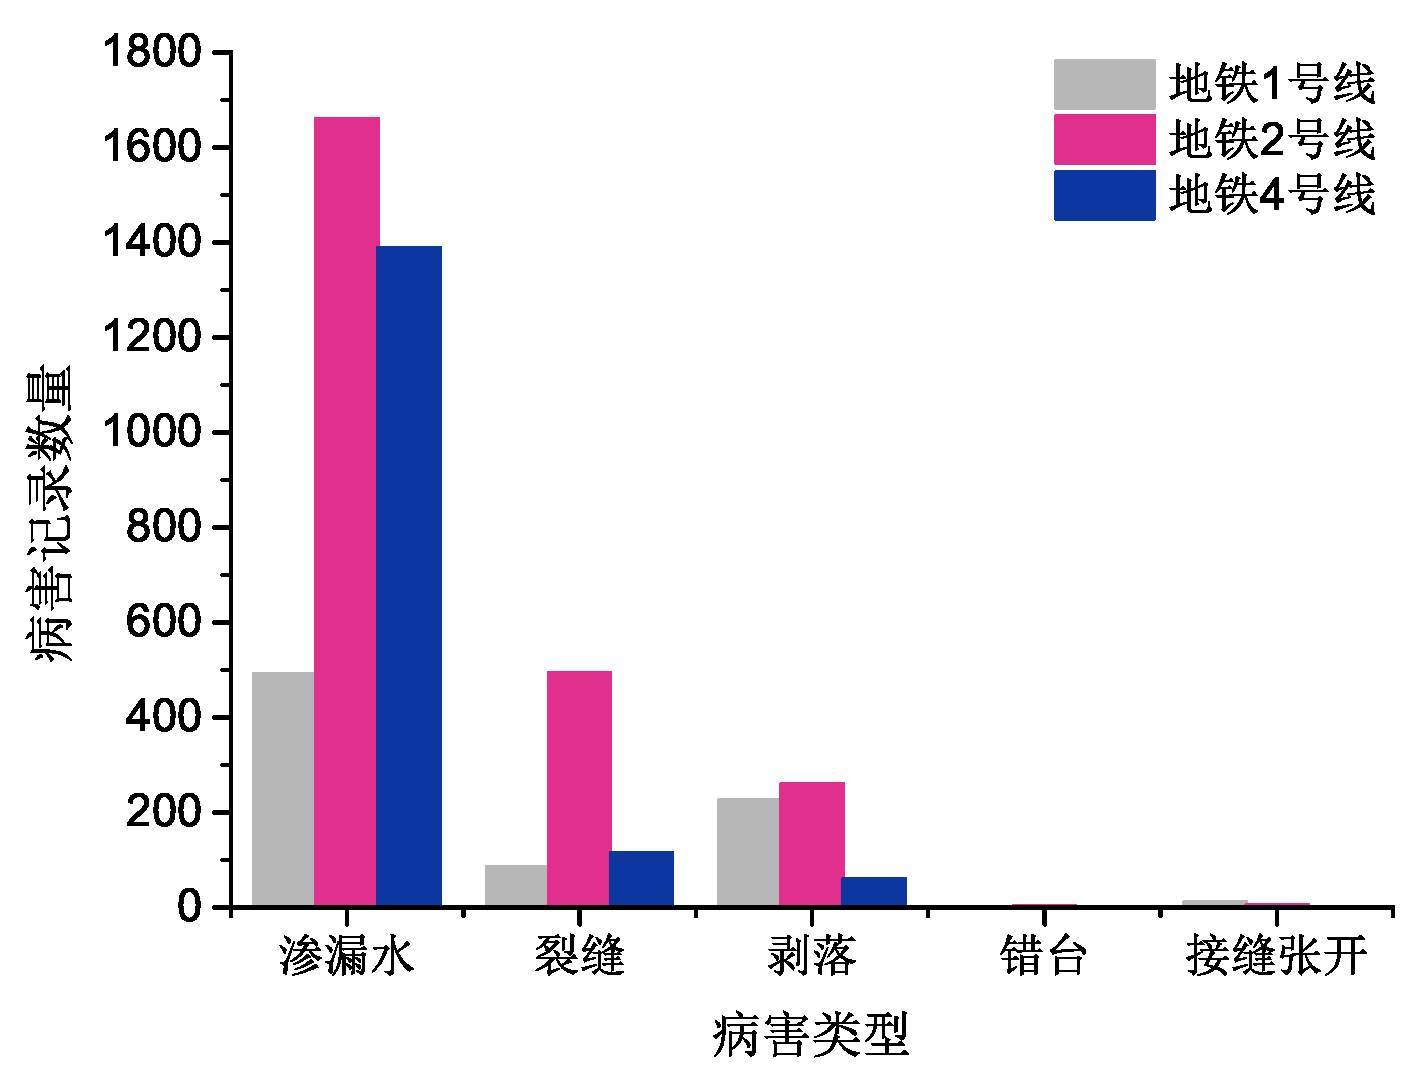
\includegraphics[width=0.8\textwidth]{chap2/distress-num.eps}
    \caption{上海地铁病害统计图}
    \label{fig:上海地铁病害统计图}
\end{figure}

另一方面,许多学者研究得出接缝张开和错台与隧道的沉降和收敛有较大相关性(Ding等,\citeyear{ding2013full};Gong等,\citeyear{gong2017comparison};彭益成等,\citeyear{彭益成2013盾构隧道衬砌结构的壳},)。王如路和张冬梅(\citeyear{王如路2013超载作用下软土盾构隧道横向变形机理及控制指标研究})根据隧道衬砌管片之间的相对位置,仅考虑管片在横向收敛时只发生相对转动和平动,采用几何学方法,得出接缝张开与横向收敛的关系,如图~\ref{fig:衬砌管片横向收敛与接缝张开几何关系图}~所示。

\begin{figure}[htbp]
    \centering
    \includegraphics[width=0.5\textwidth]{chap2/lining-geom.png}
    \caption{衬砌管片横向收敛与接缝张开几何关系图(王如路和张冬梅,\citeyear{王如路2013超载作用下软土盾构隧道横向变形机理及控制指标研究})}
    \label{fig:衬砌管片横向收敛与接缝张开几何关系图}
\end{figure}

廖少明等(\citeyear{廖少明2005隧道纵向剪切传递效应及其一维解析})根据弹性地基梁理论,提出隧道纵向剪切传递的概念,如图~\ref{fig:弹性地基梁纵向剪切平衡分析图}~所示。认为隧道的纵向不均匀沉降将导致隧道纵向变形剪切,也即是错台病害的产生。

\begin{figure}[htbp]
    \centering
    \includegraphics[width=0.9\textwidth]{chap2/sett-shear.png}
    \caption{弹性地基梁纵向剪切平衡分析图(廖少明等,\citeyear{廖少明2005隧道纵向剪切传递效应及其一维解析})}
    \label{fig:弹性地基梁纵向剪切平衡分析图}
\end{figure}

因此,本文只选取渗漏水、裂缝、剥落作为评估指标,如式~\ref{equ:leakage}~-~\ref{equ:cracking}~所示,其中:$r$为检查隧道区间总环数;${d}_{l}$为百环渗漏水面积($m^2/100$环);${d}_{s}$为百环衬砌剥落面积($m^2/100$环);${d}_{c}$为百环裂缝长度($m/100$环);${n}_{l}$为渗漏水记录总数;${n}_{s}$为剥落记录总数;${n}_{c}$为裂缝记录总数;${l}_{ai}$为第$i$个渗漏水面积;${s}_{ai}$为第$i$个剥落面积;${c}_{li}$为第$i$个裂缝长度。
\begin{align}
    \label{equ:leakage}
    {{d}_{l}}=\frac{\sum\limits_{i=1}^{{{n}_{l}}}{{{l}_{ai}}}}{r}\times 100 \\
    \label{equ:spalling}
    {{d}_{s}}=\frac{\sum\limits_{i=1}^{{{n}_{s}}}{{{s}_{ai}}}}{r}\times 100 \\
    \label{equ:cracking}
    {{d}_{c}}=\frac{\sum\limits_{i=1}^{{{n}_{c}}}{{{c}_{li}}}}{r}\times 100
\end{align}
%+++++++++++++++++++++++++++++++++++++++++++++++++++++++++++++++++%
\subsection{研究样本指标特征}

综上所述,本文选取了六个观测变量:相对沉降平均值${sett}_{a}$、平均差异沉降$set{{t}_{d\_a}}$、平均收敛变形率${cov}_{a}$、百环渗漏水面积${d}_{l}$、百环衬砌剥落面积${d}_{s}$、百环裂缝长度${d}_{c}$作为评估指标。表~\ref{tab:上海地铁观测变量统计信息}~统计了上海地铁盾构隧道上述六个观测变量的相关信息,后续的评估结果可用于与此类似的盾构隧道工程。

\begin{table}[htbp]
  \centering
  \caption{上海地铁观测变量统计信息}
    \begin{tabular}{?m{6em}<{\centering}"c"c"c"c"c"c?}
    \thickhline
    观测变量  & 最小值   & 第一四分位 & 中位数   & 第三四分位 & 最大值   & 平均值 \bigstrut\\
    \thinhline
    ${sett}_{a}$\newline($mm$)  & 1.2   & 8.2   & 19.6  & 40.2  & 150.1  & 27.8  \bigstrut\\
    \thinhline
    $set{{t}_{d\_a}}$\newline($mm/100m$) & 1.5   & 4.2   & 9.5   & 19.8  & 58.0  & 12.5  \bigstrut\\
    \thinhline
    ${cov}_{a}$\newline($‰D$)  & 2.4   & 6.1   & 7.3   & 8.4   & 12.0  & 1.5  \bigstrut\\
    \thinhline
    ${d}_{l}$\newline($m^2/100$环) & 0.00  & 0.16  & 0.42  & 1.11  & 5.74  & 0.86  \bigstrut\\
    \thinhline
    ${d}_{s}$\newline($m^2/100$环) & 0.00  & 0.00  & 0.00  & 0.90  & 5.67  & 0.76  \bigstrut\\
    \thinhline
    ${d}_{c}$\newline($m/100$环) & 0.00  & 0.00  & 0.00  & 0.01  & 1.30  & 0.08  \bigstrut\\
    \thickhline
    \end{tabular}%
  \label{tab:上海地铁观测变量统计信息}%
\end{table}%

%%%%%%%%%%%%%%%%%%%%%%%%%%%%%%%%%%%%%%%%%%%%%%%%%%%%%%%%%%%%%%%%%%%
\section{基于主成分分析和关联性分析的TSI计算公式}

%+++++++++++++++++++++++++++++++++++++++++++++++++++++++++++++++++%
\subsection{盾构隧道服役性能专家评分}

隧道服役性能评分(TSR)通过专家打分表获取,没有采用现场巡查打分的原因是地铁隧道只有在地铁停运后,凌晨的4、5个小时才能进入,现场巡查的方式并不切合实际。图~\ref{fig:隧道服役性能评分表}~所示为TSR专家打分表,选取200环衬砌作为一次评估单位,因为评估长度选择太短,区间包含的病害较少,长度太长则不能保证隧道服役性能在区间保持不变。评分表上包含了样本的基本信息,包括地铁线路、起始终止车站、起始终止环号、病害检查日期,评分表上还包含了病害的位置、大小、形状,和沉降、收敛的监测数据。Yuan等(\citeyear{Yuan2012Assessment})和盾构法隧道结构服役性能鉴定规范(\citeyear{DGTJ0821232013})将隧道服役性能等级分为正常、退化、劣化、恶化、危险五个等级,本文参考此分级方法,将隧道服役性能等级分为5个级别,分别为很好(1分)、好(2分)、一般(3分)、差(4分)、很差(5分)。

\begin{figure}[htbp]
    \centering
    \includegraphics[width=1.0\textwidth]{chap2/tsr.pdf}
    \caption{隧道服役性能评分表}
    \label{fig:隧道服役性能评分表}
\end{figure}

\begin{table}[!htbp]
  \centering
  \caption{专家评分小组成员}
    \begin{tabular}{?m{5em}<{\centering}"m{5em}<{\centering}"m{5em}<{\centering}"m{8em}<{\centering}?}
    \thickhline
    序号    & 年龄    & 工作年限  & 背景 \bigstrut\\
    \thinhline
    1     & 45    & 14    & 地铁结构设计 \bigstrut\\
    \thinhline
    2     & 44    & 21    & 地铁施工 \bigstrut\\
    \thinhline
    3     & 60    & 36    & 结构监测 \bigstrut\\
    \thinhline
    4     & 43    & 9     & 结构养护 \bigstrut\\
    \thinhline
    5     & 41    & 10    & 结构养护 \bigstrut\\
    \thinhline
    6     & 36    & 10    & 结构维护 \bigstrut\\
    \thinhline
    7     & 47    & 27    & 结构维护 \bigstrut\\
    \thinhline
    8     & 40    & 10    & 结构研究 \bigstrut\\
    \thinhline
    9     & 46    & 17    & 岩土研究 \bigstrut\\
    \thickhline
    \end{tabular}%
  \label{tab:专家评分小组成员}%
\end{table}%

评分小组由9位专家组成,分别来自设计、施工、管理、维养和研究等背景的专家,如表~\ref{tab:专家评分小组成员}~所示。在评分前,会跟专家说明隧道服役性能的基本定义和假设,且允许专家一起讨论交流各自的意见,但在评分过程中专家禁止任何交流,直到完成评分为止。该评分小组于2015年1月17日对18个样本区间进行评分,于2015年5月23日对另外21个样本区间进行评分,评分结果如表~\ref{tab:隧道服役性能评分结果}~所示,其中第40个样本是假设隧道在初始状态没有任何病害、变形,其$TSR$应为1.0,表~\ref{tab:隧道服役性能评分结果}~第2列为样本所有评分的平均值,评分范围从1.1-3.9分,第3列为样本评分的标准差,第4到8列为样本的观测变量。

\begin{longtable}{?c"c"c"c"c"c"c"c"c?}
    \caption{隧道服役性能评分结果}
    \label{tab:隧道服役性能评分结果}\\
    \thickhline
    \multirow{3}[2]{*}{序号} & \multirow{3}[2]{2.85em}{专家评分} & \multirow{3}[2]{3em}{评分\newline 标准差} & \multirow{3}[2]{2.5em}{${sett}_{a}$\newline ($mm$)} & \multirow{3}[2]{4em}{$set{{t}_{d\_a}}$\newline ($mm/$\newline 100m)} & \multirow{3}[2]{2.5em}{${cov}_{a}$\newline ($‰D$)} & \multirow{3}[2]{3.5em}{${d}_{l}$\newline ($m^2/$\newline 百环)} & \multirow{3}[2]{3.5em}{${d}_{s}$\newline ($m^2/$\newline 百环)} & \multirow{3}[2]{3.5em}{${d}_{c}$\newline($m/$\newline 百环)} \bigstrut[t]\\
          &       &       &       &       &       &       &       &  \bigstrut[b]\\
         &       &       &       &       &       &       &       &  \bigstrut[b]\\          
    \thinhline
    \endfirsthead

    \caption{隧道服役性能评分结果(续表)}
    \label{tab:隧道服役性能评分结果}\\
    \thickhline
    \multirow{3}[2]{*}{序号} & \multirow{3}[2]{2.85em}{专家评分} & \multirow{3}[2]{3em}{评分\newline 标准差} & \multirow{3}[2]{2.5em}{${sett}_{a}$\newline ($mm$)} & \multirow{3}[2]{4em}{$set{{t}_{d\_a}}$\newline ($mm/$\newline 100m)} & \multirow{3}[2]{2.5em}{${cov}_{a}$\newline ($‰D$)} & \multirow{3}[2]{3.5em}{${d}_{l}$\newline ($m^2/$\newline 百环)} & \multirow{3}[2]{3.5em}{${d}_{s}$\newline ($m^2/$\newline 百环)} & \multirow{3}[2]{3.5em}{${d}_{c}$\newline($m/$\newline 百环)} \bigstrut[t]\\
          &       &       &       &       &       &       &       &  \bigstrut[b]\\
         &       &       &       &       &       &       &       &  \bigstrut[b]\\ 
    \thinhline
    \endhead

    \thickhline
    \multicolumn{9}{r}{下页续表}
    \endfoot

    \thickhline
    \endlastfoot

    1     & 2.7   & 0.7   & 10.4  & 26.4  & 3.9   & 0.35  & 0.00  & 0.00  \bigstrut\\
    \hline
    2     & 2.3   & 1.0   & 10.4  & 4.2   & 7.8   & 5.55  & 0.00  & 0.00  \bigstrut\\
    \hline
    3     & 1.1   & 0.3   & 2.4   & 4.9   & 2.8   & 0.00  & 0.00  & 0.00  \bigstrut\\
    \hline
    4     & 1.7   & 0.5   & 5.3   & 8.4   & 3.8   & 4.60  & 0.00  & 0.00  \bigstrut\\
    \hline
    5     & 3.4   & 0.9   & 88.6  & 21.6  & 8.5   & 0.70  & 0.00  & 0.00  \bigstrut\\
    \hline
    6     & 2.9   & 0.8   & 43.6  & 12.9  & 6.8   & 1.95  & 0.44  & 0.05  \bigstrut\\
    \hline
    7     & 2.7   & 0.7   & 25.5  & 12.9  & 9.2   & 1.05  & 1.03  & 0.15  \bigstrut\\
    \hline
    8     & 1.9   & 0.4   & 10.8  & 17.3  & 5.6   & 0.00  & 0.00  & 0.00  \bigstrut\\
    \hline
    9     & 3.5   & 1.0   & 125.3  & 17.4  & 9.4   & 0.20  & 4.19  & 0.05  \bigstrut\\
    \hline
    10    & 2.7   & 0.9   & 27.3  & 8.0   & 8.0   & 0.35  & 0.44  & 0.05  \bigstrut\\
    \hline
    11    & 1.7   & 0.5   & 25.0  & 2.5   & 3.5   & 0.90  & 0.00  & 0.00  \bigstrut\\
    \hline
    12    & 1.9   & 0.4   & 6.9   & 19.6  & 4.5   & 0.00  & 0.00  & 0.05  \bigstrut\\
    \hline
    13    & 2.3   & 1.1   & 6.6   & 23.3  & 5.1   & 5.80  & 0.00  & 0.00  \bigstrut\\
    \hline
    14    & 2.1   & 0.8   & 15.1  & 27.2  & 7.3   & 0.00  & 2.33  & 0.00  \bigstrut\\
    \hline
    15    & 2.0   & 1.0   & 32.4  & 3.3   & 7.9   & 2.05  & 0.36  & 0.05  \bigstrut\\
    \hline
    16    & 2.7   & 0.5   & 16.0  & 23.3  & 4.1   & 5.75  & 0.00  & 0.00  \bigstrut\\
    \hline
    17    & 1.2   & 0.4   & 5.3   & 9.0   & 4.4   & 0.00  & 0.00  & 0.05  \bigstrut\\
    \hline
    18    & 1.3   & 0.5   & 3.6   & 1.2   & 3.1   & 0.00  & 0.00  & 0.00  \bigstrut\\
    \hline
    19    & 1.8   & 0.7   & 31.5  & 3.7   & 4.1   & 1.35  & 0.00  & 0.00  \bigstrut\\
    \hline
    20    & 3.3   & 0.4   & 69.3  & 10.7  & 5.7   & 0.25  & 1.14  & 0.05  \bigstrut\\
    \hline
    21    & 1.3   & 0.5   & 3.2   & 17.5  & 5.0   & 0.95  & 0.00  & 0.00  \bigstrut\\
    \hline
    22    & 2.3   & 0.7   & 38.1  & 8.3   & 6.5   & 0.25  & 0.33  & 0.00  \bigstrut\\
    \hline
    23    & 2.3   & 0.9   & 15.6  & 25.6  & 6.0   & 2.50  & 0.00  & 0.00  \bigstrut\\
    \hline
    24    & 4.0   & 0.7   & 131.4  & 29.2  & 6.8   & 1.95  & 0.66  & 0.15  \bigstrut\\
    \hline
    25    & 3.5   & 0.7   & 96.6  & 40.5  & 8.1   & 0.70  & 0.67  & 0.10  \bigstrut\\
    \hline
    26    & 2.5   & 0.5   & 22.8  & 4.9   & 6.2   & 0.00  & 1.35  & 0.00  \bigstrut\\
    \hline
    27    & 2.0   & 0.5   & 20.3  & 4.5   & 7.9   & 0.35  & 0.00  & 0.05  \bigstrut\\
    \hline
    28    & 2.0   & 0.3   & 25.0  & 20.4  & 7.2   & 0.00  & 0.00  & 0.10  \bigstrut\\
    \hline
    29    & 2.3   & 0.7   & 9.2   & 26.4  & 3.6   & 5.75  & 0.00  & 0.00  \bigstrut\\
    \hline
    30    & 3.3   & 1.1   & 50.3  & 23.3  & 7.5   & 0.00  & 0.63  & 0.05  \bigstrut\\
    \hline
    31    & 2.0   & 0.6   & 7.1   & 26.1  & 6.4   & 0.75  & 0.00  & 0.11  \bigstrut\\
    \hline
    32    & 1.5   & 0.5   & 12.5  & 6.0   & 3.5   & 0.00  & 0.00  & 0.00  \bigstrut\\
    \hline
    33    & 3.4   & 0.9   & 142.0  & 57.0  & 9.1   & 0.00  & 0.36  & 0.00  \bigstrut\\
    \hline
    34    & 2.3   & 0.7   & 5.0   & 6.4   & 7.3   & 1.55  & 1.12  & 0.05  \bigstrut\\
    \hline
    35    & 3.1   & 0.8   & 33.9  & 4.3   & 10.2  & 1.20  & 0.00  & 0.00  \bigstrut\\
    \hline
    36    & 3.1   & 0.8   & 75.6  & 21.6  & 7.6   & 0.70  & 0.00  & 0.15  \bigstrut\\
    \hline
    37    & 3.9   & 0.8   & 143.2  & 54.2  & 9.2   & 0.25  & 2.36  & 0.15  \bigstrut\\
    \hline
    38    & 3.1   & 0.9   & 43.2  & 27.1  & 7.1   & 0.00  & 1.13  & 0.10  \bigstrut\\
    \hline
    39    & 2.5   & 0.7   & 18.8  & 27.9  & 5.3   & 2.75  & 0.00  & 0.00  \bigstrut\\
    \hline
    40    & 1.0   & 0.0   & 0.0   & 0.0   & 0.0   & 0.00  & 0.00  & 0.00  \bigstrut\\
\end{longtable}

%+++++++++++++++++++++++++++++++++++++++++++++++++++++++++++++++++%
\subsection{TSI评估指标体系的线性化处理}

\begin{figure}[htbp!] 
    \centering 
    \begin{tabular}{c} 
        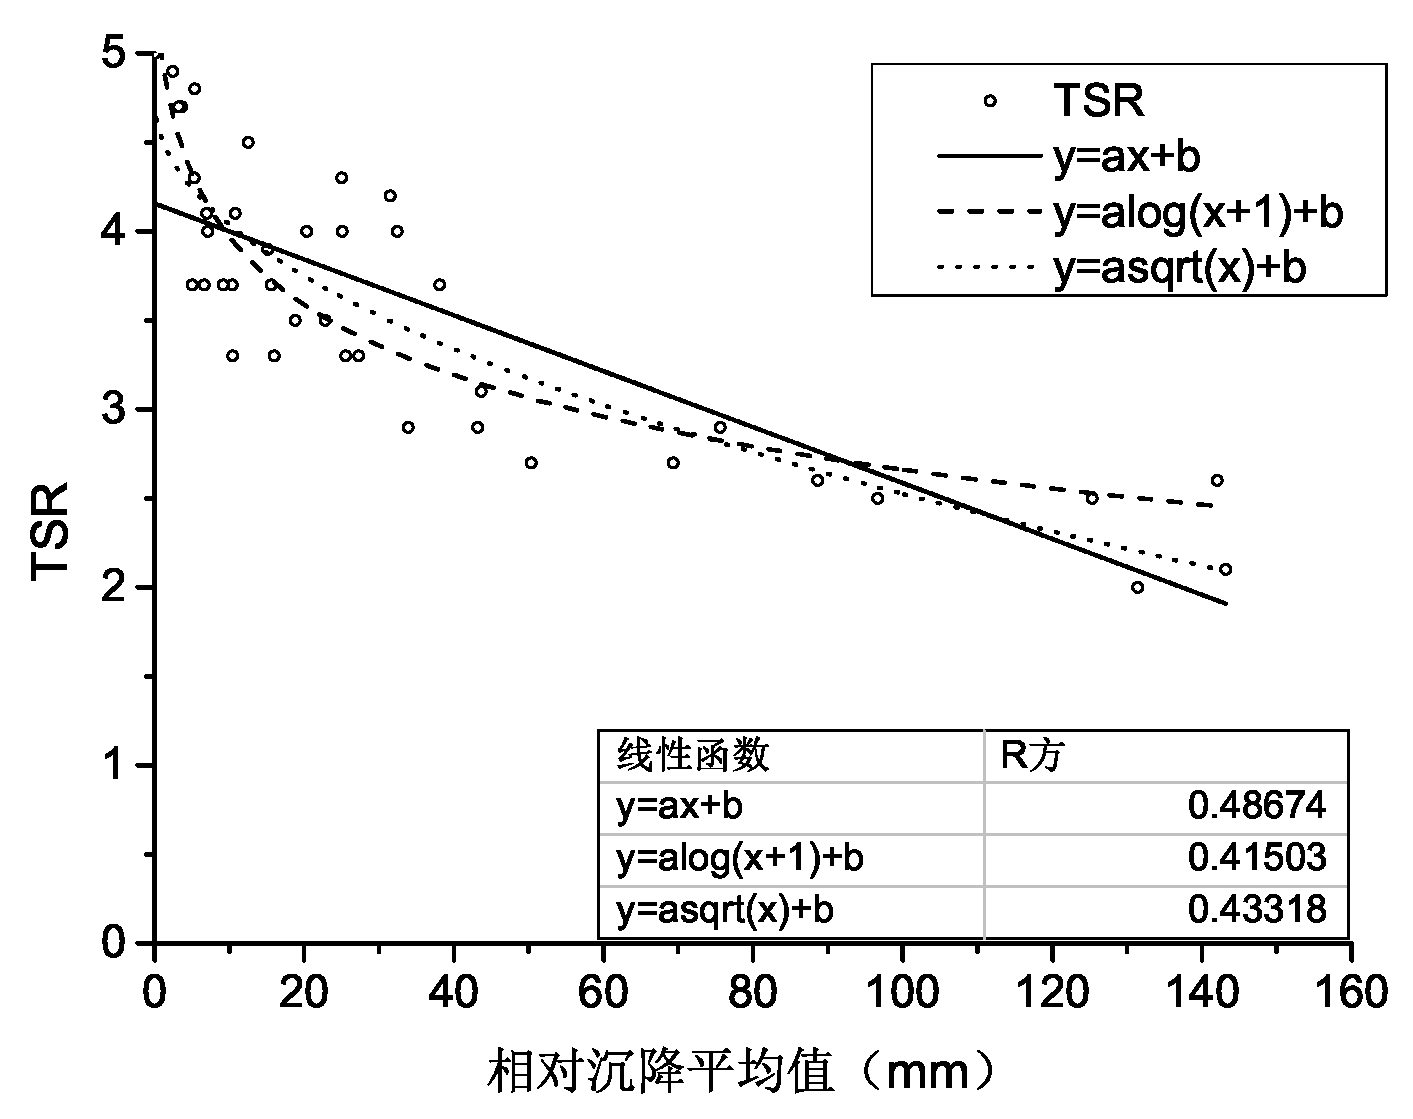
\includegraphics[width=0.6\textwidth]{chap2/tsr-setta.eps} \\ 
        (a)~专家评分-${sett}_{a}$ \\
        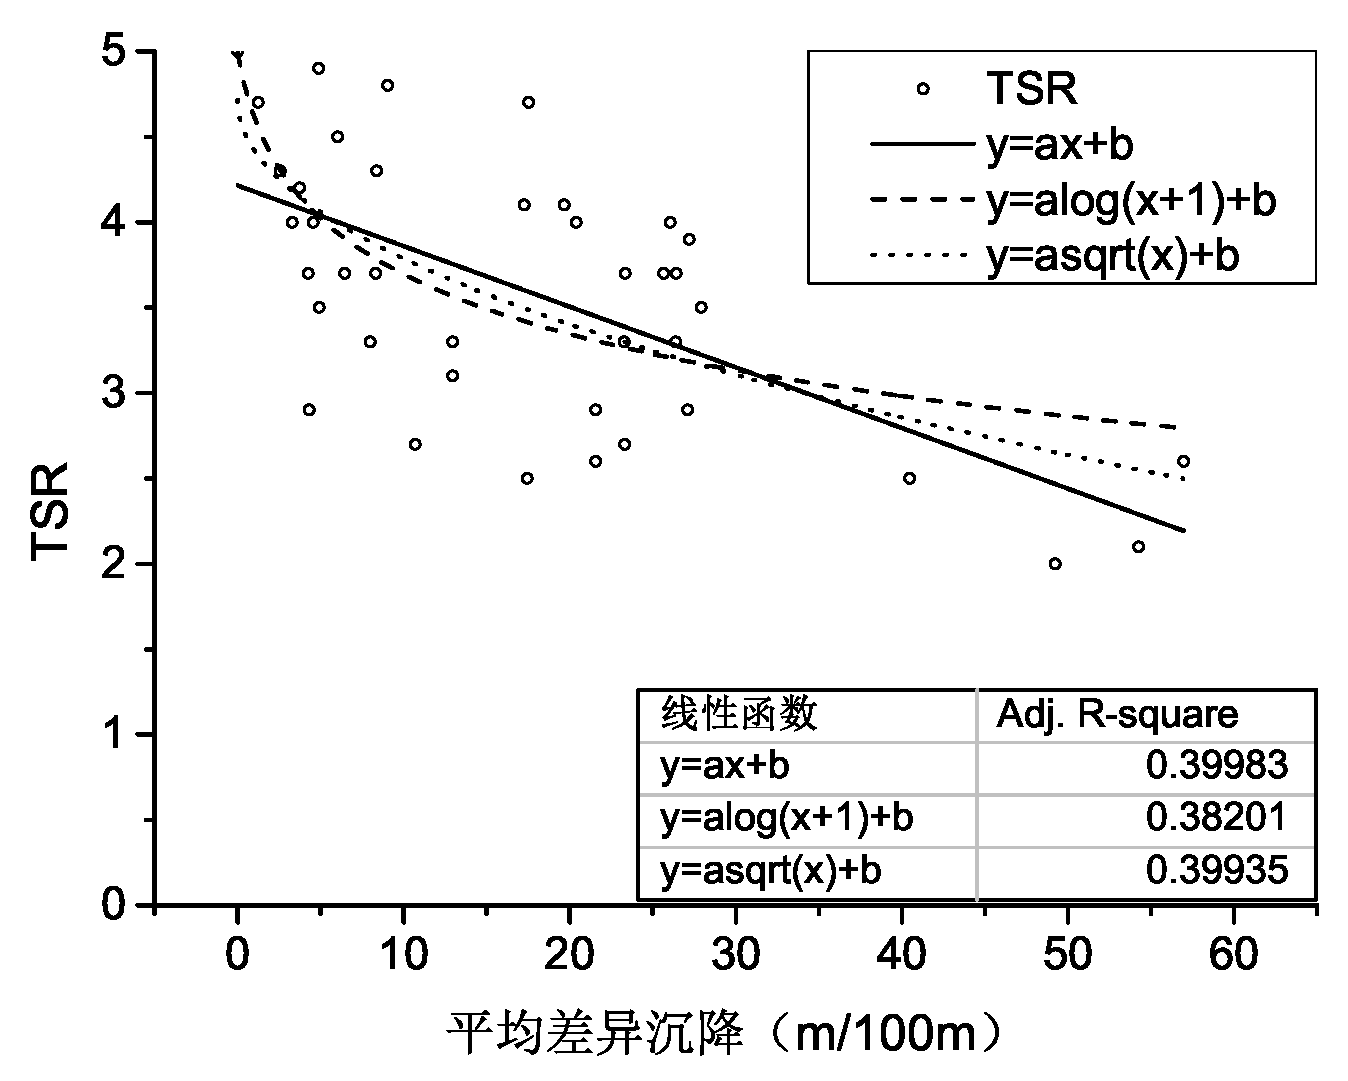
\includegraphics[width=0.6\textwidth]{chap2/tsr-settr.eps} \\ 
        (b)~专家评分-$set{{t}_{d\_a}}$ \\
        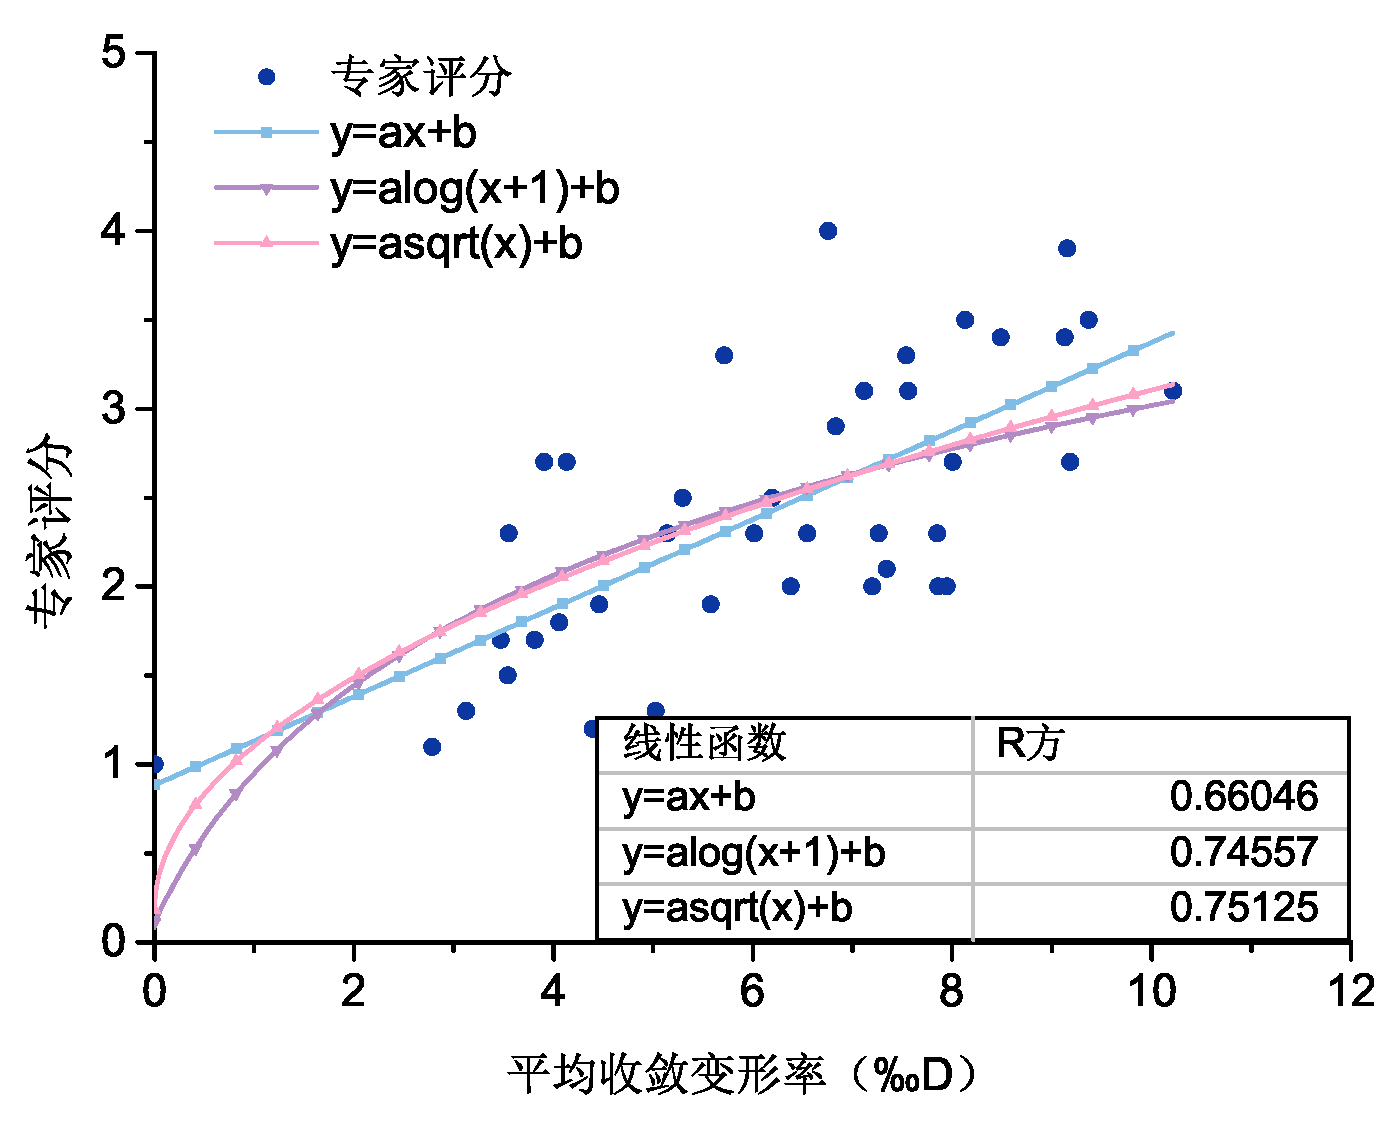
\includegraphics[width=0.6\textwidth]{chap2/tsr-conv.eps} \\ 
        (c)~专家评分-${cov}_{a}$ \\
    \end{tabular}
    \caption{专家评分与观测变量关系图} 
    \label{fig:TSR与观测变量关系图} 
\end{figure}

\begin{figure}[htbp!] 
    \centering 
    \begin{tabular}{c} 
        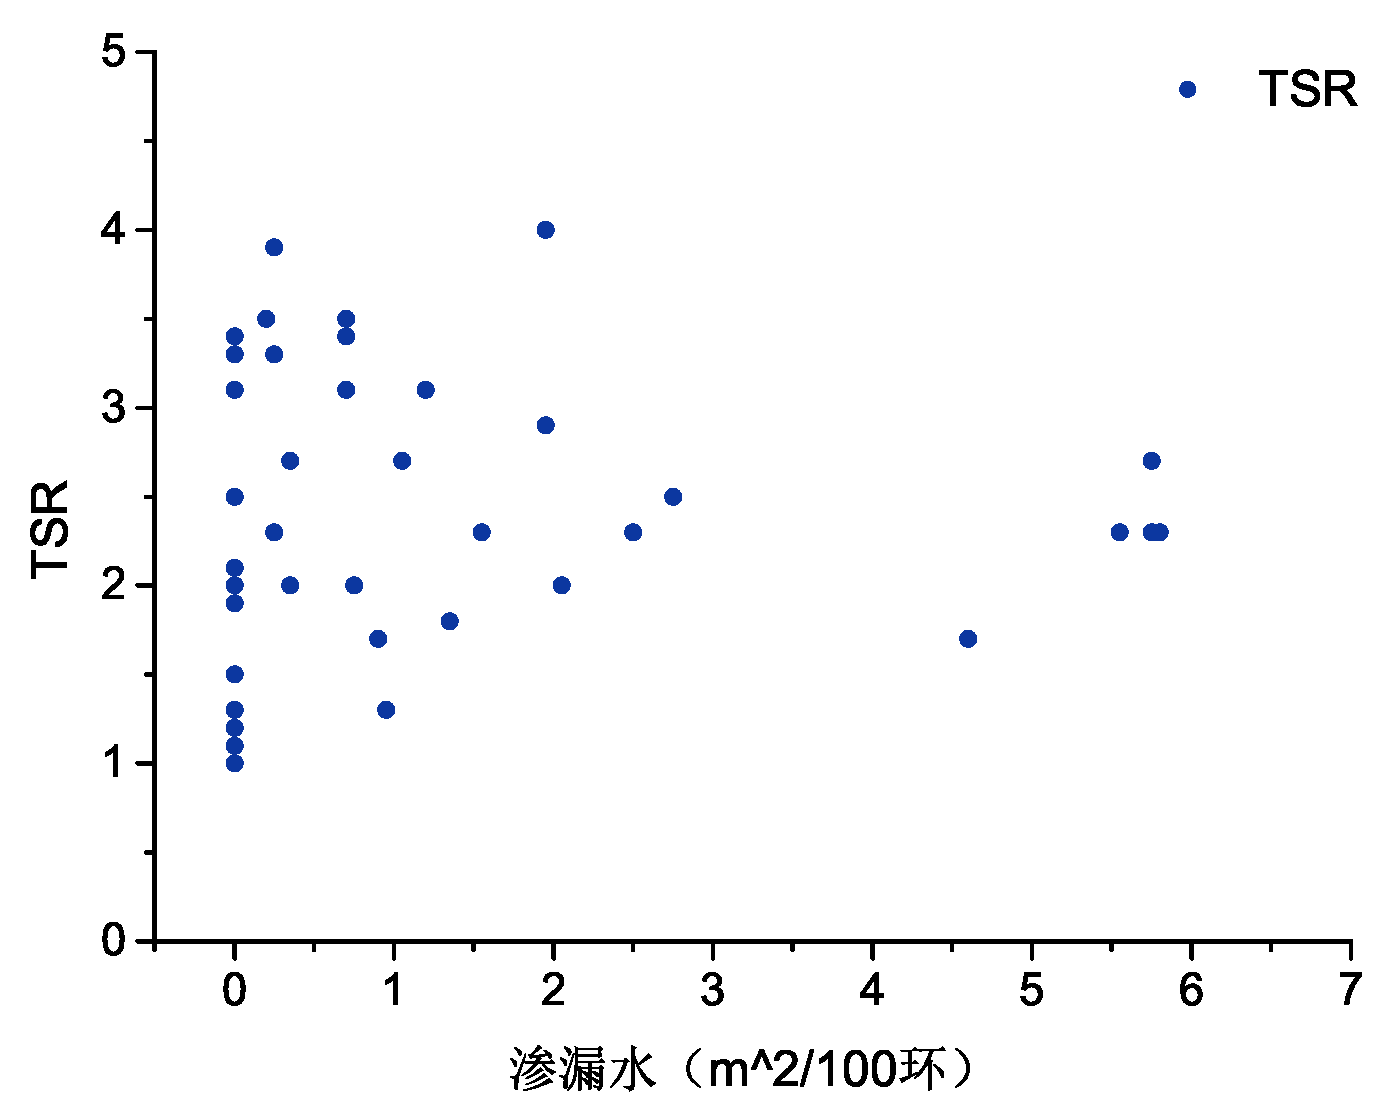
\includegraphics[width=0.59\textwidth]{chap2/tsr-leakge.eps} \\ 
        (a)~专家评分-${d}_{l}$ \\
        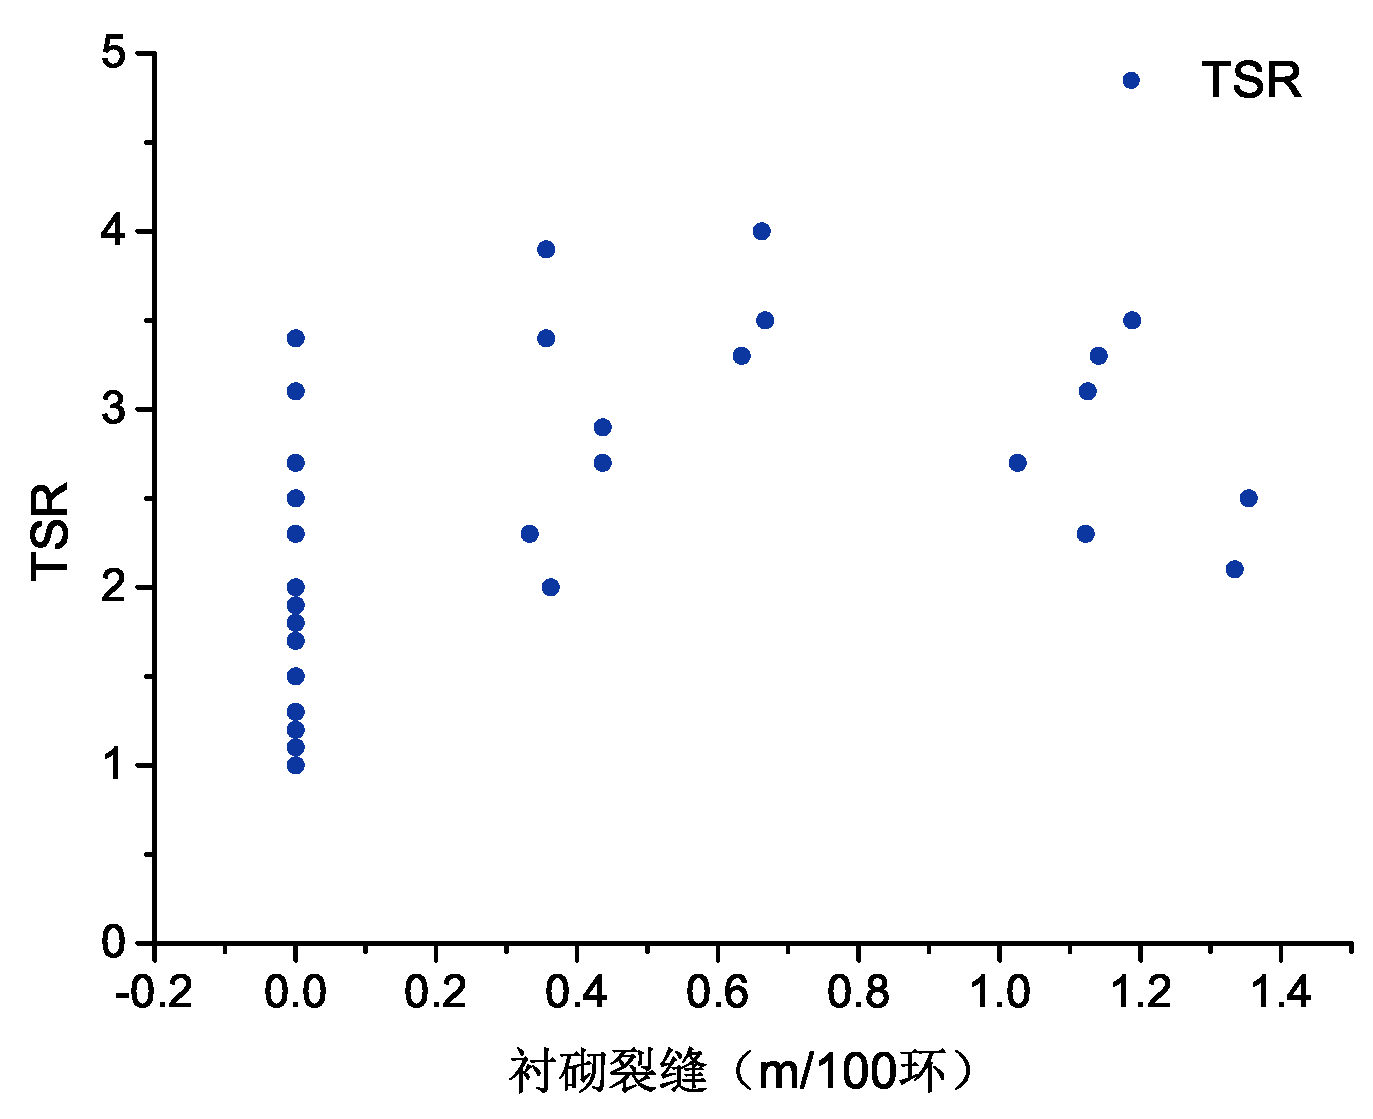
\includegraphics[width=0.59\textwidth]{chap2/tsr-spall.eps} \\ 
        (b)~专家评分-$d_s$ \\
        \includegraphics[width=0.59\textwidth]{chap2/tsr-crack.eps} \\ 
        (c)~专家评分-$d_c$ \\
    \end{tabular}
    \caption{专家评分与观测变量关系图} 
    \label{fig:TSR与观测变量关系图2} 
\end{figure}

多元回归方法一般都是多元线性回归分析,对于与因变量成非线性关系的自变量需通过函数变换线性化。图~\ref{fig:TSR与观测变量关系图}~展示了各个观测变量与专家评分的散点图,分别采用线性函数、对数函数和平方根函数对观测变量进行线性化处理,采用确定系数$R^2$来反映回归结果的拟合优度。图~\ref{fig:TSR与观测变量关系图}a~线性函数、对数函数和平方根函数的拟合结果分别为0.67、0.74和0.75。故在多元回归时将${sett}_{a}$转换为$\sqrt{sett_a}$。由图~\ref{fig:TSR与观测变量关系图}b~和图~\ref{fig:TSR与观测变量关系图}c~可知,线性函数对$set{{t}_{d\_a}}$和${cov}_{a}$的拟合度最高,分别为0.40和0.49。但是对于${d}_{l}$、$d_s$和$d_c$三个观测变量,从图~\ref{fig:TSR与观测变量关系图2}~中可看出与TSR不存在明显的函数关系,故无需对其作线性变化。

%+++++++++++++++++++++++++++++++++++++++++++++++++++++++++++++++++%
\subsection{基于主成分分析和关联性分析拟合方法}

一般地,多元线性回归模型的自变量的基本要求是:在模型中应包含所有对因变量有重要解析意义的因素,并且自变量之间不存在线性相关的现象。若自变量之间存在严重的线性相关性,普通的最小二乘法拟合回归模型将不能保证回归结果的精确性和可靠性。而偏最小二乘回归能较好解决这一问题,其结合了主成分分析和典型相关性分析理论,能够在自变量存在相关性的条件下进行回归建模,同时更易识别系统信息与噪声。

偏最小二乘法的主要思想如下:设有$q$个因变量$\{{{y}_{1}},{{y}_{2}},\cdots ,{{y}_{q}}\}$和$p$个自变量$\{{{x}_{1}},{{x}_{2}},\cdots ,{{x}_{p}}\}$,为了研究因变量与自变量的统计关系,假设收集$n$个样本,则构成的自变量和因变量空间为$X={{[{{x}_{1}},\cdots ,{{x}_{p}}]}_{n\times p}}$和$Y={{[{{y}_{1}},\cdots ,{{y}_{q}}]}_{n\times q}}$。偏最小二乘是从$X$和$Y$中提取主成分$t_1$和$u_1$,即$t_1$是${{x}_{1}},\cdots ,{{x}_{p}}$的线性组合,$u_1$是${{y}_{1}},\cdots ,{{y}_{q}}$的线性组合,再进行线性回归时应满足下述两个要求:

(1)$t_1$和$u_1$应尽可能的携带$X$和$Y$中的变异信息;

(2)$t_1$和$u_1$之间的相关程度应尽可能大。

上述两个要求表明,$t_1$和$u_1$应尽可能好的代表数据$X$和$Y$,同时$t_1$对$u_1$又有较强的解释能力。在第一个成分被提取后,分别实施$X$对$t_1$和$Y$对$u_1$的回归。如果回归方程已经达到满意的精度,则得到结果;否则,利用$X$去除$t_1$的残余信息和$Y$去除$u_1$的残余信息循环进行成分提取,直到结果满意为止。下面简略说明偏最小二乘法的计算推导,更详细的推导内容可以参考相关书籍(Tobias,\citeyear{tobias1995introduction};王慧文,\citeyear{王惠文1999偏最小二乘回归方法及其应用})。

第一步:记${{E}_{0}}={{({{E}_{01}},\cdots ,{{E}_{0p}})}_{n\times p}}$为$X$经标准化处理后的矩阵,${{F}_{0}}={{({{F}_{01}},\cdots ,{{F}_{0q}})}_{n\times q}}$为$Y$经标准化处理后的矩阵;记$t_1$为${{E}_{0}}$第一主成分,$t_1={E_0}{w_1}$,$w_1$为$E_0$第一个轴,且$\left\| {{w}_{1}} \right\|=1$;记$u_1$为${{F}_{0}}$第一主成分,$u_1={F_0}{c_1}$,$c_1$为$F_0$第一个轴,且$\left\| {{c}_{1}} \right\|=1$。

如果要$t_1$、$u_1$能分别很好地代表$X$、$Y$中的数据变异信息,根据主成分分析原理(Wold,\citeyear{wold1987principal}),可得
\begin{align}
    \label{equ:variance1}
    Var({{t}_{1}})\to \max \\
    \label{equ:variance2}
    Var({{u}_{1}})\to \max
\end{align}
另一方面,要求$t_1$对$u_1$有最大的解释能力,根据典型相关分析理论(Thompson,\citeyear{thompson2005canonical}),$t_1$和$u_1$的相关度应达到最大,即
\begin{equation}
    \label{equ:relation}
    r({{t}_{1}},{{u}_{1}})\to \max 
\end{equation}
综上所示,即要求$t_1$对$u_1$的协方差最大,有
\begin{equation}
    \label{equ:relation}
    Cov({{t}_{1}},{{u}_{1}})=\sqrt{Var({{t}_{1}})Var({{u}_{1}})}r({{t}_{1}},{{u}_{1}})\to \max =\max \left\langle {{t}_{1}},{{u}_{1}} \right\rangle
\end{equation}

记${{\theta }_{1}}\text{=}\left\langle {{t}_{1}},{{u}_{1}} \right\rangle =\left\langle {{E}_{0}}{{w}_{1}},{{F}_{0}}{{c}_{1}} \right\rangle$,根据拉格朗日算法可推导出,$w_1$是矩阵${{{E}'}_{0}}{{F}_{0}}{{{F}'}_{0}}{{E}_{0}}$的特征向量,对应的特征值为$\theta _{1}^{2}$。根据式~\ref{equ:relation}~可知$\theta _{1}$要求取值最大,故$w_1$是对应矩阵${{{E}'}_{0}}{{F}_{0}}{{{F}'}_{0}}{{E}_{0}}$最大特征值的单位特征向量,同理$c_1$是对应矩阵${{{F}'}_{0}}{{E}_{0}}{{{E}'}_{0}}{{F}_{0}}$最大特征值的单项特征向量。

求得轴$w_1$和$c_1$后,即可得到成分
\begin{align}
    \label{equ:pc1}
    t_1={E_0}{w_1} \\
    \label{equ:pc2}
    u_1={F_0}{c_1}
\end{align}
然后可分别求$E_0$和$F_0$对$t_1$的回归方程
\begin{align}
    \label{equ:regress1}
    E_0={t_1}{p'_1}+E_1 \\
    \label{equ:regress2}
    F_0={t_1}{r'_1}+F_1
\end{align}
式中:$E_1$和$F_1$为残差矩阵;回归系数向量是
\begin{align}
    \label{equ:regress-index1}
    {{p}_{1}}=\frac{{{{{E}'}}_{0}}{{t}_{1}}}{{{\left\| {{t}_{1}} \right\|}^{2}}} \\
    \label{equ:regress-index2}
    {{r}_{1}}=\frac{{{{{F}'}}_{0}}{{t}_{1}}}{{{\left\| {{t}_{1}} \right\|}^{2}}}
\end{align}
    
第二步:用残差矩阵$E_1$和$F_1$取代$E_0$和$F_0$,求第二个轴$w_2$和$c_2$和第二个主成分$t_2$和$u_2$,同理第一步,可求出
\begin{align}
    \label{equ:regress3}
    E_1={t_2}{p'_2}+E_2 \\
    \label{equ:regress4}
    F_1={t_2}{r'_2}+F_2
\end{align}

如此计算下去,如果$X$的秩为$A$,最终可得
\begin{align}
    \label{equ:regress5}
    {{E}_{0}}={{t}_{1}}{{{p}'}_{1}}+\cdots +{{t}_{A}}{{{p}'}_{A}} \\
    \label{equ:regress6}
    {{F}_{0}}={{t}_{1}}{{{r}'}_{1}}+\cdots {{t}_{A}}{{{r}'}_{A}}+{{F}_{A}}
\end{align}

由于$t_1,\cdots ,t_A$均可以表示成${E}_{01},\cdots ,{E}_{0p}$的线性组合,因此式~\ref{equ:regress6}~可以写成$y_k=F_{0k}$关于$x_j=E_{0j}$的线性回归方程,即
\begin{equation}
    \label{equ:regress7}
    {{y}_{k}}={{a}_{k1}}{{x}_{1}}+\cdots +{{a}_{kp}}{{x}_{p}}+{{F}_{Ak}},k=1,2,\cdots ,q
\end{equation}
式中:$y_k$为矩阵$Y$的第$k$列;$a_{ki}$为$y_k$对应第$i$个自变量的系数;${F}_{Ak}$是残差矩阵$F_A$的第$k$列。

第三步:交叉有效性验证。首先将全部$n$个样本分成两个部分,第一部分是除去某个样本点$i$的其他样本点集合,用这部分样本点采用$h$个成分拟合回归方程;第二部分则把除去的一个样本点$i$带入拟合回归方程,得到$y_i$在样本$i$的拟合值${{\hat{y}}_{hj(-i)}}$。对于所有样本重复上述过程,可定义$y_i$的预测误差平方和为
\begin{equation}
    \label{equ:press}
    {PRESS_{hj}}=\sum\limits_{t=1}^{n}{\left( {{y}_{ij}}-{{{\hat{y}}}_{hj\text{-}i}} \right)}
\end{equation}
定义$Y$的预测误差平方和为
\begin{equation}
    {{PRESS}_{h}}=\sum\limits_{j=1}^{p}{{{PRESS}_{hj}}}
\end{equation}

另外,再采用所有样本点,拟合$h$个成分的回归方程。记第$i$个样本的预测值为${{\hat{y}}_{hji}}$,可以定义$y_j$的误差平方和为
\begin{equation}
    S{{S}_{hj}}=\sum\limits_{i=1}^{n}{{{\left( {{y}_{ij}}-\hat{y}_{hji} \right)}^{2}}}
\end{equation}
定义$Y$的误差平方和为
\begin{equation}
    S{{S}_{h}}=\sum\limits_{j=1}^{p}{S{{S}_{hj}}}
\end{equation}

对于全部因变量$Y$,成分$t_h$的交叉有效性定义为
\begin{equation}
    Q_{h}^{2}=1-\frac{\sum\limits_{k=1}^{q}{PRES{{S}_{hk}}}}{\sum\limits_{k=1}^{q}{S{{S}_{(h-1)k}}}}=1-\frac{PRES{{S}_{h}}}{S{{S}_{(h-1)}}}
\end{equation}
一般认为,当$Q_{h}^{2}\ge (1-{{0.95}^{2}})=0.0975$时,添加$t_h$对拟合效果的贡献是显著的。对于$k=1,2,\cdots ,q$,至少有一个$k$,使得
\begin{equation}
    Q_{hk}^{2}\ge 0.0975
\end{equation}
这时增加成分$t_h$,至少使得一个$y_k$的拟合模型得到显著的改善,因此可以考虑增加一个主成分$t_h$。

%+++++++++++++++++++++++++++++++++++++++++++++++++++++++++++++++++%
\subsection{TSI拟合结果与有效性验证}

参考道路工程领域相关研究成果(AASHO,\citeyear{AASHO1962the}),在大量道路区间评估样本的试算基础下,评估指标的线性组合可拟合评估结果,本章也采用线性组合的模型对TSI进行拟合,并在此基础上结合主成分分析和典型相关性分析理论,考虑指标关联性的影响。根据表~\ref{tab:隧道服役性能评分结果}~的评分结果和线性化处理结果,取$X=\left[ \sqrt{set{{t}_{a}}},set{{t}_{d\_a}},{{\operatorname{cov}}_{a}},{{d}_{l}},{{d}_{c}},{{d}_{s}} \right]$,$Y=\left[ TSI \right]$,TSI公式的形式应为
\begin{gather}
    TSI={{A}_{1}}\sqrt{set{{t}_{a}}}+{{A}_{2}}set{{t}_{d\_a}}+{{B}_{1}}{{\operatorname{cov}}_{a}}+{{C}_{1}}{{d}_{l}}+{{C}_{2}}{{d}_{c}}+{{C}_{3}}{{d}_{s}}+C \\ 
    TSR=TSI+{\varepsilon }
\end{gather}
式中:$A_1$,$A_2$,$B_1$,$C_1$,$C_2$,$C_3$和$C$均为待评估的系数;$\varepsilon $为回归模型不能解释的残差。由于隧道变形和病害的增多,必然造成隧道服役性能的降低,对应TSI值应变大,所以上述的评估系数应为正数。

为消除指标之间不同量纲的影响,采取标准公式如式~\ref{equ:标准化公式}~所示,其中$\mu$为样本的平均值,$\delta$为样本的标准差,根据表~\ref{tab:隧道服役性能评分结果}~可得个评估指标的标准化公式~\ref{equ:tsi标准化}-\ref{equ:ds标准化}
\begin{gather}
 \label{equ:标准化公式} 
    {\xi }_{v}=\frac{v-\mu }{\delta }\\
  \label{equ:tsi标准化}
    {\xi }_{TSI}=\frac{TSI-{{\mu }_{TSI}}}{{{\delta }_{TSI}}}=\frac{TSI-2.4}{0.8} \\ 
  \label{equ:setta标准化}
    {\xi }_{\sqrt{set{{{{t}}}_{a}}}}=\frac{\sqrt{set{{t}_{a}}}-{{\mu }_{setta}}}{{{\delta }_{setta}}}=\frac{\sqrt{set{{t}_{a}}}-5.2}{3.1} \\ 
 \label{equ:settda标准化}
    {\xi }_{set{{{{t}}}_{d\_a}}}=\frac{set{{t}_{d\_a}}-{{\mu }_{settda}}}{{{\delta }_{settda}}}=\frac{set{{t}_{d\_a}}-17.2}{13.4} \\ 
 \label{equ:cova标准化}
    {\xi }_{cov_a}=\frac{{{\operatorname{cov}}_{a}}-{{\mu }_{\operatorname{cov}a}}}{{{\delta }_{\operatorname{cov}a}}}=\frac{{cov_a}-6.1}{2.2} \\ 
 \label{equ:dl标准化}
    {\xi }_{{{{d}}}_{l}}=\frac{{{d}_{l}}-{{\mu }_{dl}}}{{{\delta }_{dl}}}=\frac{{{d}_{l}}-1.3}{1.8} \\ 
 \label{equ:dc标准化}
    {\xi }_{{{{d}}}_{c}}=\frac{{{d}_{c}}-{{\mu }_{dc}}}{{{\delta }_{dc}}}=\frac{{{d}_{c}}-0.5}{0.9} \\ 
 \label{equ:ds标准化}
    {\xi }_{{{{d}}}_{s}}=\frac{{{d}_{s}}-{{\mu }_{ds}}}{{{\delta }_{ds}}}=\frac{{{d}_{s}}-0}{0.1}
\end{gather}
式中:${\xi }_{set{{{{t}}}_{a}}}$,${\xi }_{set{{{t}}_{d\_a}}}$,${\xi }_{cov_a}$,${\xi }_{{d}_{c}}$,${\xi }_{{{d}}_{s}}$分别为${set{{t}_{a}}}$,$set{{t}_{d\_a}}$,${cov_a}$,${{d}_{l}}$,${{d}_{c}}$,${{d}_{s}}$的标准化公式。

根据式~\ref{equ:regress1}-\ref{equ:regress-index2}~可计算得TSI的标准化公式和TSI公式
\begin{align}
  \label{tsi-std}
  & {\xi }_{TSI}=0.62{\xi }_{\sqrt{set{{{{t}}}_{a}}}}+0.13{\xi }_{set{{{{t}}}_{d\_a}}}+0.25{\xi }_{cov_a} \\ 
 & \quad \quad \quad +0.19{\xi }_{{{{d}}}_{l}}+0.06{\xi }_{{d}_{c}}+0.03{\xi }_{{{{d}}}_{s}} \nonumber
\end{align}

由标准化公式~\ref{tsi-std}~可知,累积沉降平均值指标所占比重对大,权重系数为0.62,即其在六个指标当中是最重要的,其次为平均收敛率、渗漏水、平均差异沉降。衬砌剥落和衬砌裂缝两个指标的权重较小,主要原因是专家认为目前上海地铁盾构隧道的大部分剥落和裂缝病害并不是运营期间产生的,而是由于施工期的不当操作造成,且在运营期这类病害并没有劣化的趋势。

最终可根据~\ref{equ:tsi标准化}-\ref{equ:ds标准化}~计算TSI公式如式~\ref{tsi}~,参考上海地铁观测变量统计表~\ref{tab:上海地铁观测变量统计信息}~,可得TSI公式各评估指标的取值范围:
\begin{gather}
  \label{tsi}
  TSI=0.77+0.16\sqrt{set{{t}_{a}}}+0.01set{{t}_{d\_a}}+0.09{{\operatorname{cov}}_{a}} \\ 
  +0.08{{d}_{l}}+0.05{{d}_{c}}+0.50{{d}_{s}}\text{,其中:}  \nonumber \\
  0\le set{{t}_{a}}\le 150mm \nonumber \\
  0\le set{{t}_{d\_a}}\le 60mm/100m \nonumber \\
  0\le cov_a\le 12‰D \nonumber \\
  0\le d_l\le 6m^2/100\text{环} \nonumber \\
  0\le d_s\le 6m^2/100\text{环} \nonumber \\
  0\le d_c\le 1.5m/100\text{环} \nonumber
\end{gather}

图~\ref{fig:TSI和TSR的比较与关系}~所示为评分样本的TSI和TSR关系与比较。图~\ref{fig:TSI和TSR的比较与关系}a~描述了公式~\ref{tsi}~的拟合度,$R^2$为$0.841$,即公式~\ref{tsi}~解释了84.1\%的评分样本数据。图~\ref{fig:TSI和TSR的比较与关系}b~所示为样本的TSI计算值与TSR值比较,图中可以看出,除了1号样本和15号样本,其余样本的TSI与TSR差值均在0.5以内。

\begin{figure}[htb!] 
    \centering 
    \begin{tabular}{c} 
        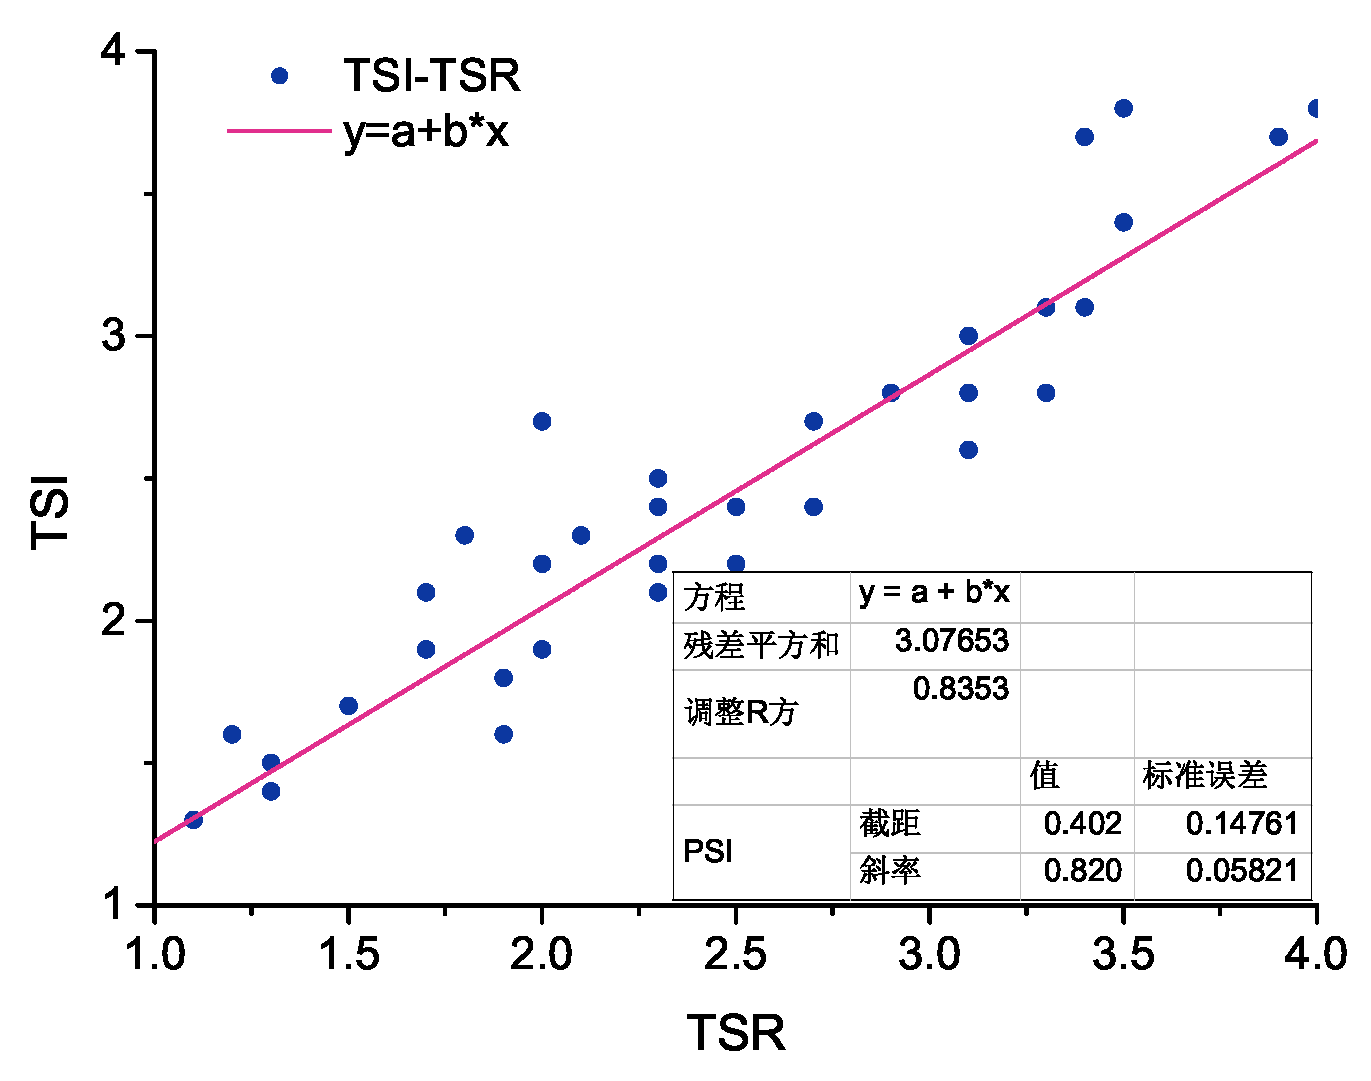
\includegraphics[width=0.7\textwidth]{chap2/tsi-tsr.eps} \\ 
    \end{tabular}
    \caption{评分样本TSI和TSR的比较与关系} 
    \label{fig:TSI和TSR的比较与关系} 
\end{figure}

为验证TSI公式结果的有效性,选择常用的盾构法隧道结构服役性能鉴定规范(DG/TJ08-2123-2013,\citeyear{DGTJ0821232013};GB50157,\citeyear{GB501572013})和模糊层次综合评价法(陈楠,\citeyear{陈楠2017考虑发展趋势与指标关联的隧道结构健康评估方法研究})进行结果对比,对比样本选择表~\ref{tab:隧道服役性能评分结果}~所示的盾构隧道样本,三种方法的计算结果如表~\ref{tab:隧道服役性能TSI结果对比}~所示,规范的评估方法较模糊层次综合评价和TSI公式要保守,当某一指标严重劣化时,将导致评估结果至最差等级,TSI公式的评估结果与模糊层次综合评价结果类似,对比图如图~\ref{fig:1-20号样本不同评估方法结果比较}~和图~\ref{fig:21-40号样本不同评估方法结果比较}~所示。TSI公式的优点在于:(1)TSI是一个综合性指标,且该指标尽量少地引入主观因素;(2)TSI公式的形式更简单,计算更加便捷。

\begin{longtable}{?c"c"c"c"c"c"c"c"c"c?}
    \caption{隧道服役性能TSI结果对比}
    \label{tab:隧道服役性能TSI结果对比}\\
    \thickhline
    \multirow{2}[2]{*}{序号} & \multirow{2}[2]{2.5em}{${sett}_{a}$} & \multirow{2}[2]{2.5em}{$set{{t}_{d\_a}}$} & \multirow{2}[2]{2.5em}{${cov}_{a}$} & \multirow{2}[2]{2.5em}{${d}_{l}$} & \multirow{2}[2]{2.5em}{${d}_{c}$} & \multirow{2}[2]{2.5em}{${d}_{s}$} & \multicolumn{1}{c"}{\multirow{2}[2]{2.6em}{TSI}} & \multicolumn{1}{c"}{\multirow{2}[2]{2.6em}{规范}} & \multicolumn{1}{c?}{\multirow{2}[2]{4em}{模糊层次\newline 综合评价}} \bigstrut[t]\\
      &       &       &       &       &       &       &       &       &  \bigstrut[b]\\
    \thinhline
    \endfirsthead

    \caption{隧道服役性能TSI结果对比(续表)}
    \label{tab:隧道服役性能TSI结果对比}\\
    \thickhline
    \multirow{2}[2]{*}{序号} & \multirow{2}[2]{2.5em}{${sett}_{a}$} & \multirow{2}[2]{2.5em}{$set{{t}_{d\_a}}$} & \multirow{2}[2]{2.5em}{${cov}_{a}$} & \multirow{2}[2]{2.5em}{${d}_{l}$} & \multirow{2}[2]{2.5em}{${d}_{c}$} & \multirow{2}[2]{2.5em}{${d}_{s}$} & \multicolumn{1}{c"}{\multirow{2}[2]{2.6em}{TSI}} & \multicolumn{1}{c"}{\multirow{2}[2]{2.6em}{规范}} & \multicolumn{1}{c?}{\multirow{2}[2]{4em}{模糊层次\newline 综合评价}} \bigstrut[t]\\
      &       &       &       &       &       &       &       &       &  \bigstrut[b]\\
    \thinhline
    \endhead

    \thickhline
    \multicolumn{10}{r}{下页续表}
    \endfoot

    \thickhline
    \endlastfoot

    1     & 10.4  & 26.4  & 3.9   & 0.35  & 0.00  & 0.00  & 1.9   & 1     & 1 \bigstrut\\
    \hline
    2     & 10.4  & 4.2   & 7.8   & 5.55  & 0.00  & 0.00  & 2.5   & 4     & 2 \bigstrut\\
    \hline
    3     & 2.4   & 4.9   & 2.8   & 0.00  & 0.00  & 0.00  & 1.3   & 1     & 1 \bigstrut\\
    \hline
    4     & 5.3   & 8.4   & 3.8   & 4.60  & 0.00  & 0.00  & 1.9   & 3     & 2 \bigstrut\\
    \hline
    5     & 88.6  & 21.6  & 8.5   & 0.70  & 0.00  & 0.00  & 3.3   & 3     & 3 \bigstrut\\
    \hline
    6     & 43.6  & 12.9  & 6.8   & 1.95  & 0.44  & 0.05  & 2.8   & 2     & 2 \bigstrut\\
    \hline
    7     & 25.5  & 12.9  & 9.2   & 1.05  & 1.03  & 0.15  & 2.7   & 4     & 4 \bigstrut\\
    \hline
    8     & 10.8  & 17.3  & 5.6   & 0.00  & 0.00  & 0.00  & 2.0   & 2     & 1 \bigstrut\\
    \hline
    9     & 125.3  & 17.4  & 9.4   & 0.20  & 4.19  & 0.05  & 3.8   & 5     & 4 \bigstrut\\
    \hline
    10    & 27.3  & 8.0   & 8.0   & 0.35  & 0.44  & 0.05  & 2.5   & 3     & 3 \bigstrut\\
    \hline
    11    & 25.0  & 2.5   & 3.5   & 0.90  & 0.00  & 0.00  & 2.0   & 1     & 1 \bigstrut\\
    \hline
    12    & 6.9   & 19.6  & 4.5   & 0.00  & 0.00  & 0.05  & 1.8   & 1     & 1 \bigstrut\\
    \hline
    13    & 6.6   & 23.3  & 5.1   & 5.80  & 0.00  & 0.00  & 2.3   & 4     & 3 \bigstrut\\
    \hline
    14    & 15.1  & 27.2  & 7.3   & 0.00  & 2.33  & 0.00  & 2.4   & 5     & 4 \bigstrut\\
    \hline
    15    & 32.4  & 3.3   & 7.9   & 2.05  & 0.36  & 0.05  & 2.6   & 2     & 3 \bigstrut\\
    \hline
    16    & 16.0  & 23.3  & 4.1   & 5.75  & 0.00  & 0.00  & 2.5   & 4     & 4 \bigstrut\\
    \hline
    17    & 5.3   & 9.0   & 4.4   & 0.00  & 0.00  & 0.05  & 1.7   & 1     & 1 \bigstrut\\
    \hline
    18    & 3.6   & 1.2   & 3.1   & 0.00  & 0.00  & 0.00  & 1.4   & 1     & 1 \bigstrut\\
    \hline
    19    & 31.5  & 3.7   & 4.1   & 1.35  & 0.00  & 0.00  & 2.2   & 2     & 2 \bigstrut\\
    \hline
    20    & 69.3  & 10.7  & 5.7   & 0.25  & 1.14  & 0.05  & 2.8   & 4     & 2 \bigstrut\\
    \hline
    21    & 3.2   & 17.5  & 5.0   & 0.95  & 0.00  & 0.00  & 1.8   & 2     & 1 \bigstrut\\
    \hline
    22    & 38.1  & 8.3   & 6.5   & 0.25  & 0.33  & 0.00  & 2.5   & 2     & 2 \bigstrut\\
    \hline
    23    & 15.6  & 25.6  & 6.0   & 2.50  & 0.00  & 0.00  & 2.4   & 2     & 2 \bigstrut\\
    \hline
    24    & 131.4  & 29.2  & 6.8   & 1.95  & 0.66  & 0.15  & 3.8   & 5     & 3 \bigstrut\\
    \hline
    25    & 96.6  & 40.5  & 8.1   & 0.70  & 0.67  & 0.10  & 3.6   & 4     & 3 \bigstrut\\
    \hline
    26    & 22.8  & 4.9   & 6.2   & 0.00  & 1.35  & 0.00  & 2.2   & 4     & 2 \bigstrut\\
    \hline
    27    & 20.3  & 4.5   & 7.9   & 0.35  & 0.00  & 0.05  & 2.3   & 2     & 3 \bigstrut\\
    \hline
    28    & 25.0  & 20.4  & 7.2   & 0.00  & 0.00  & 0.10  & 2.5   & 2     & 1 \bigstrut\\
    \hline
    29    & 9.2   & 26.4  & 3.6   & 5.75  & 0.00  & 0.00  & 2.3   & 4     & 3 \bigstrut\\
    \hline
    30    & 50.3  & 23.3  & 7.5   & 0.00  & 0.63  & 0.05  & 2.9   & 2     & 3 \bigstrut\\
    \hline
    31    & 7.1   & 26.1  & 6.4   & 0.75  & 0.00  & 0.11  & 2.1   & 2     & 2 \bigstrut\\
    \hline
    32    & 12.5  & 6.0   & 3.5   & 0.00  & 0.00  & 0.00  & 1.7   & 1     & 1 \bigstrut\\
    \hline
    33    & 142.0  & 57.0  & 9.1   & 0.00  & 0.36  & 0.00  & 4.1   & 5     & 5 \bigstrut\\
    \hline
    34    & 5.0   & 6.4   & 7.3   & 1.55  & 1.12  & 0.05  & 2.1   & 4     & 3 \bigstrut\\
    \hline
    35    & 33.9  & 4.3   & 10.2  & 1.20  & 0.00  & 0.00  & 2.8   & 4     & 4 \bigstrut\\
    \hline
    36    & 75.6  & 21.6  & 7.6   & 0.70  & 0.00  & 0.15  & 3.2   & 3     & 3 \bigstrut\\
    \hline
    37    & 143.2  & 54.2  & 9.2   & 0.25  & 2.36  & 0.15  & 4.3   & 5     & 5 \bigstrut\\
    \hline
    38    & 43.2  & 27.1  & 7.1   & 0.00  & 1.13  & 0.10  & 2.8   & 4     & 2 \bigstrut\\
    \hline
    39    & 18.8  & 27.9  & 5.3   & 2.75  & 0.00  & 0.00  & 2.4   & 2     & 2 \bigstrut\\
    \hline
    40    & 0.0   & 0.0   & 0.0   & 0.00  & 0.00  & 0.00  & 0.8   & 1     & 1 \bigstrut\\
\end{longtable}

\begin{figure}[htbp]
    \centering
    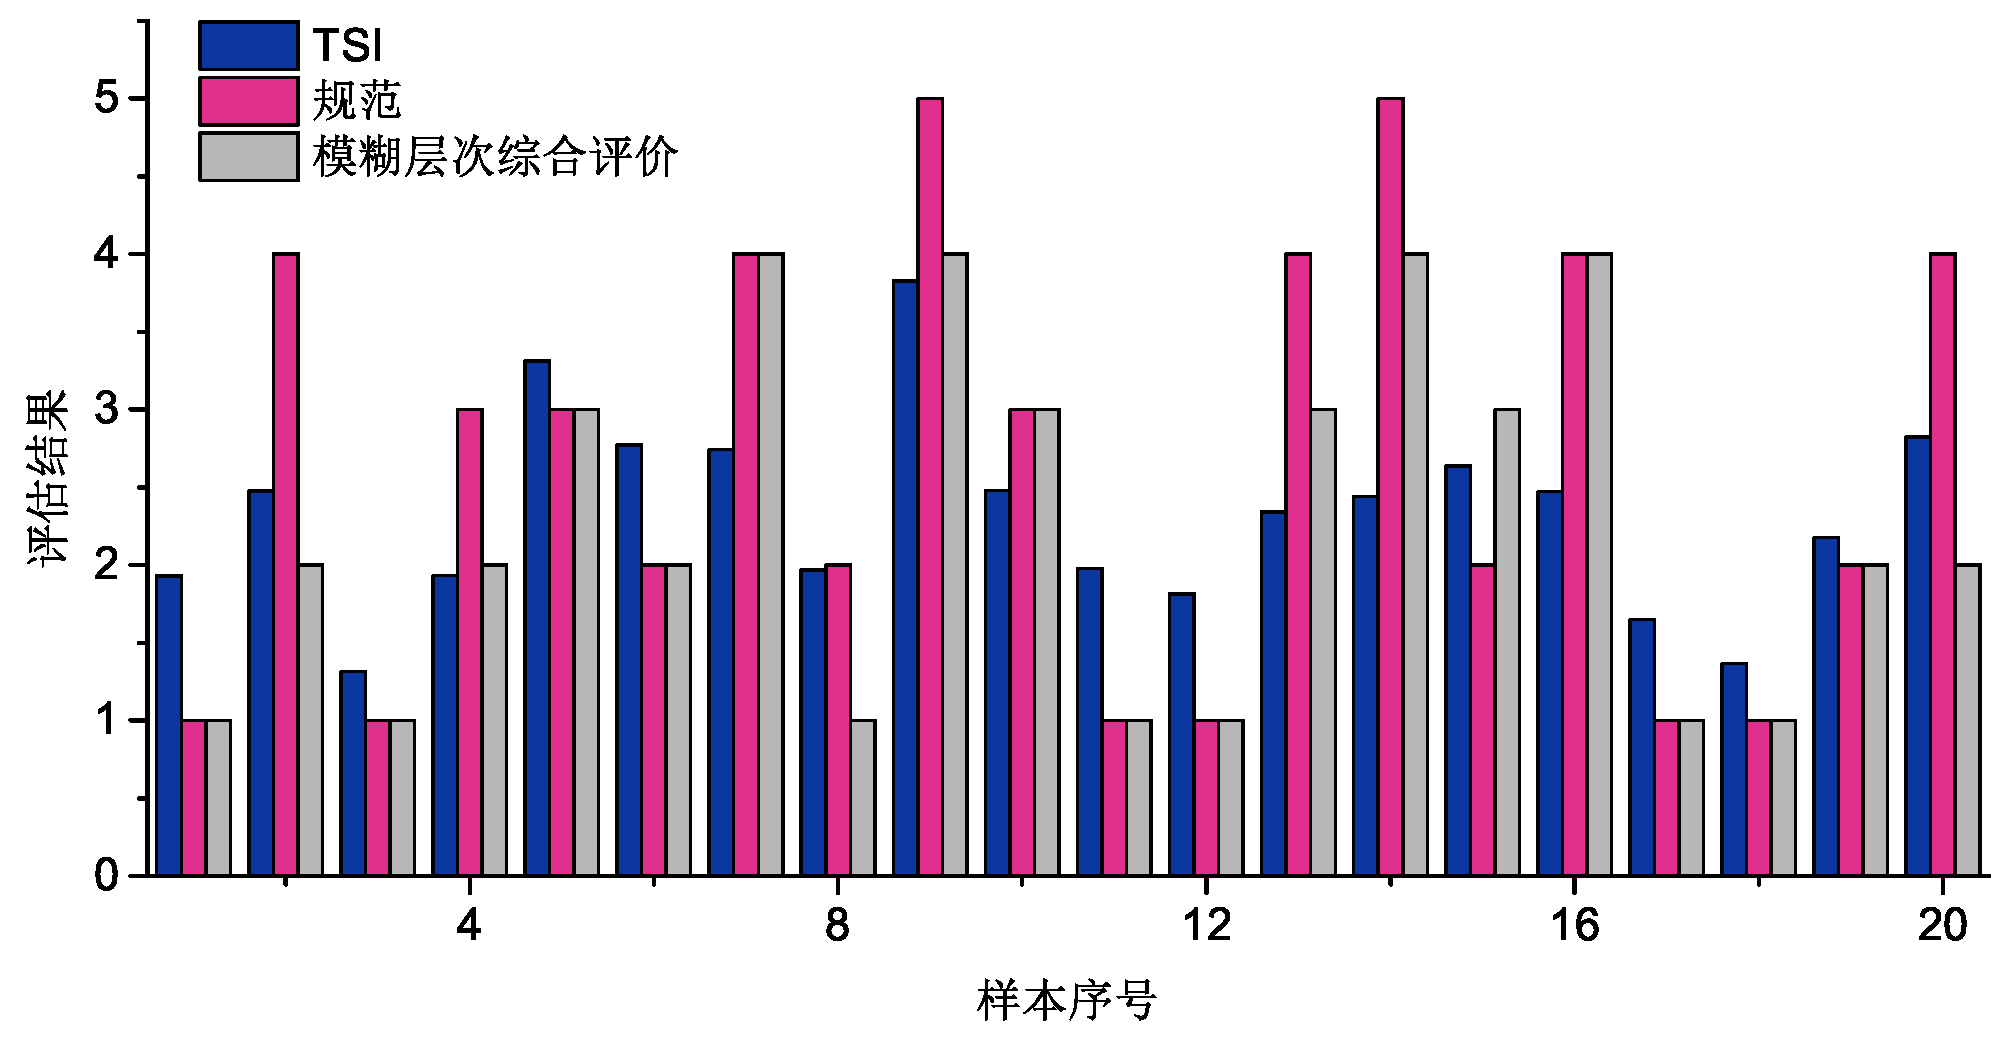
\includegraphics[width=1.0\textwidth]{chap2/compare1.eps}
    \caption{1-20号样本不同评估方法结果比较}
    \label{fig:1-20号样本不同评估方法结果比较}
\end{figure}

\begin{figure}[htbp]
    \centering
    \includegraphics[width=1.0\textwidth]{chap2/compare2.eps}
    \caption{21-40号样本不同评估方法结果比较}
    \label{fig:21-40号样本不同评估方法结果比较}
\end{figure}

%%%%%%%%%%%%%%%%%%%%%%%%%%%%%%%%%%%%%%%%%%%%%%%%%%%%%%%%%%%%%%%%%%%
\section{TSI评估与上海地铁TSI结果统计}
\label{chap:tsi-maintenance}

结合专家意见,TSI计算结果与隧道评估等级关系如下:TSI小于等于1.5对应评估状态为“很好”,病害程度基本为无或者非常轻微,对隧道运营安全无影响;TSI在1.6-2.5范围对应评估状态为“好”,病害程度轻微,对运营安全尚无影响;TSI在2.6-3.5范围对应评估状态为“一般”,病害程度中等,可能即将影响隧道运营安全,应尽快实施特殊监测,针对运营期隧道结构病害段开展的结构及周边环境的监测;TSI在3.6-4.5范围对应评估状态为“差”,病害程度较严重,已经影响隧道运营安全,应按需限制使用;TSI大于4.5对应状态“很差”,病害程度严重,严重影响对到运营安全,应限制使用,对隧道进行详细评估。各等级对照如表~\ref{tab:TSI与评估等级对照表}~所示。

\begin{table}[htb!]
  \centering
  \caption{TSI与评估等级对照表}
    \begin{tabular}{?p{3.5em}<{\centering}"m{2.5em}<{\centering}"p{4.19em}"p{9em}"p{14em}?}
    \thickhline
    TSI   & 状态    & 病害程度  & 病害对运营安全影响 & \multicolumn{1}{m{14em}<{\centering}?}{养护措施} \bigstrut\\
    \thinhline
    $\le $1.5 & 很好    & 无或者非常轻微 & 无影响   & 无 \bigstrut\\
    \thinhline
    1.6 - 2.5 & 好     & 轻微    & 目前尚无影响 & 在下次检查中重点调查 \bigstrut\\
    \thinhline
    2.6 - 3.5 & 一般    & 中等    & 将来影响运营安全 & 尽快实施特殊监测,依据监测结果确定是否采取维修措施 \bigstrut\\
    \thinhline
    3.6 - 4.5 & 差     & 较严重   & 已经影响运营安全 & 按需要限制使用,尽快采取维修措施,维修完成前实施特殊检查 \bigstrut\\
    \thinhline
    > 4.5 & 很差    & 严重    & 严重影响运营安全 & 限制使用,进行维修、更换或重建,同时实施特殊检查 \bigstrut\\
    \thickhline
    \end{tabular}%
  \label{tab:TSI与评估等级对照表}%
\end{table}%

对于“差”和“很差”状态,再分四个亚级,TSI在3.6-3.9范围的隧道区间,应及时采取特殊监测,对隧道区间进行重点保护;TSI在4.0-4.5范围,应启动专项检查,基于日常检查、定期检查和特殊检查的结果,对重点病害段进行检查;TSI在4.6-4.9范围,除了采取专项检查以外,还应成立专项研究,对隧道重点病害建立各类损伤模型,进行详细评估;TSI在5.0以上则立即限制隧道使用,并根据具体情况实施维修、更换或重建。

\begin{table}[htb!]
  \centering
  \caption{差和很差状态亚级分类}
    \begin{tabular}{?c"m{4.5em}<{\centering}"m{6em}<{\centering}"p{16em}?}
    \thickhline
    \multicolumn{1}{?m{3.5em}<{\centering}"}{状态} & 亚级    & 养护措施  & \multicolumn{1}{m{16em}<{\centering}?}{备注} \bigstrut\\
    \thinhline
    \multicolumn{1}{?c"}{\multirow{2}[4]{*}{差}} & 3.6 - 3.9 & 特殊监测  & 对隧道区间进行重点保护 \bigstrut\\
\cline{2-4}          & 4.0 - 4.5 & 专项检查  & 基于日常检查、定期检查和特殊检查的结果,对重点病害段的检查 \bigstrut\\
    \thinhline
    \multicolumn{1}{?c"}{\multirow{2}[4]{*}{很差}} & 4.6 - 4.9 & 专项检查,专项研究 & 对隧道建立各类损伤模型评估 \bigstrut\\
\cline{2-4}          & > 5.0 & 立即限制使用 & 进行维修、更换或重建 \bigstrut\\
    \thickhline
    \end{tabular}%
  \label{tab:差和很差状态亚级分类}%
\end{table}%

以上海地铁盾构隧道为例,统计地铁1号线、2号线和4号线隧道区间TSI计算结果,并给出不同评估状态的指标范围分布情况,由于目前样本的评估结果大部分在“很好”、“好”和“一般”级别,本节只统计这三种状态,如图~\ref{fig:上海地铁隧道TSI评估结果统计}~所示,对于相对沉降,“很好”状态样本均在10$mm$以下,“好”状态样本80\%以上在10-50$mm$范围,“一般”状态样本80\%以上在30-150$mm$;对于差异沉降,“很好”和“好”状态样本的指标分布类似,大部分在5-30$mm/100m$范围,“一般”状态样本则在15-50$mm/100m$范围内;对于收敛变形,“很好”状态样本在3-6$‰D$,“好”状态样本80\%在4-10$‰D$,“一般”状态样本80\%在6-12$‰D$。对于渗漏水、裂缝和剥落等病害数据的统计可见图~\ref{fig:上海地铁隧道TSI评估结果统计2}~。

另外根据TSI计算公式,可计算不同评估指标数值大小对应的TSI值,选取四个较为重要的评估指标:相对沉降、差异沉降、收敛变形和渗漏水组合绘制评估指标数值与TSI关系,如图~\ref{fig:评估指标数值与TSI结果关系}~和图~\ref{fig:评估指标数值与TSI结果关系2}~所示。

\begin{figure}[htbp!] 
    \centering 
    \begin{tabular}{c} 
        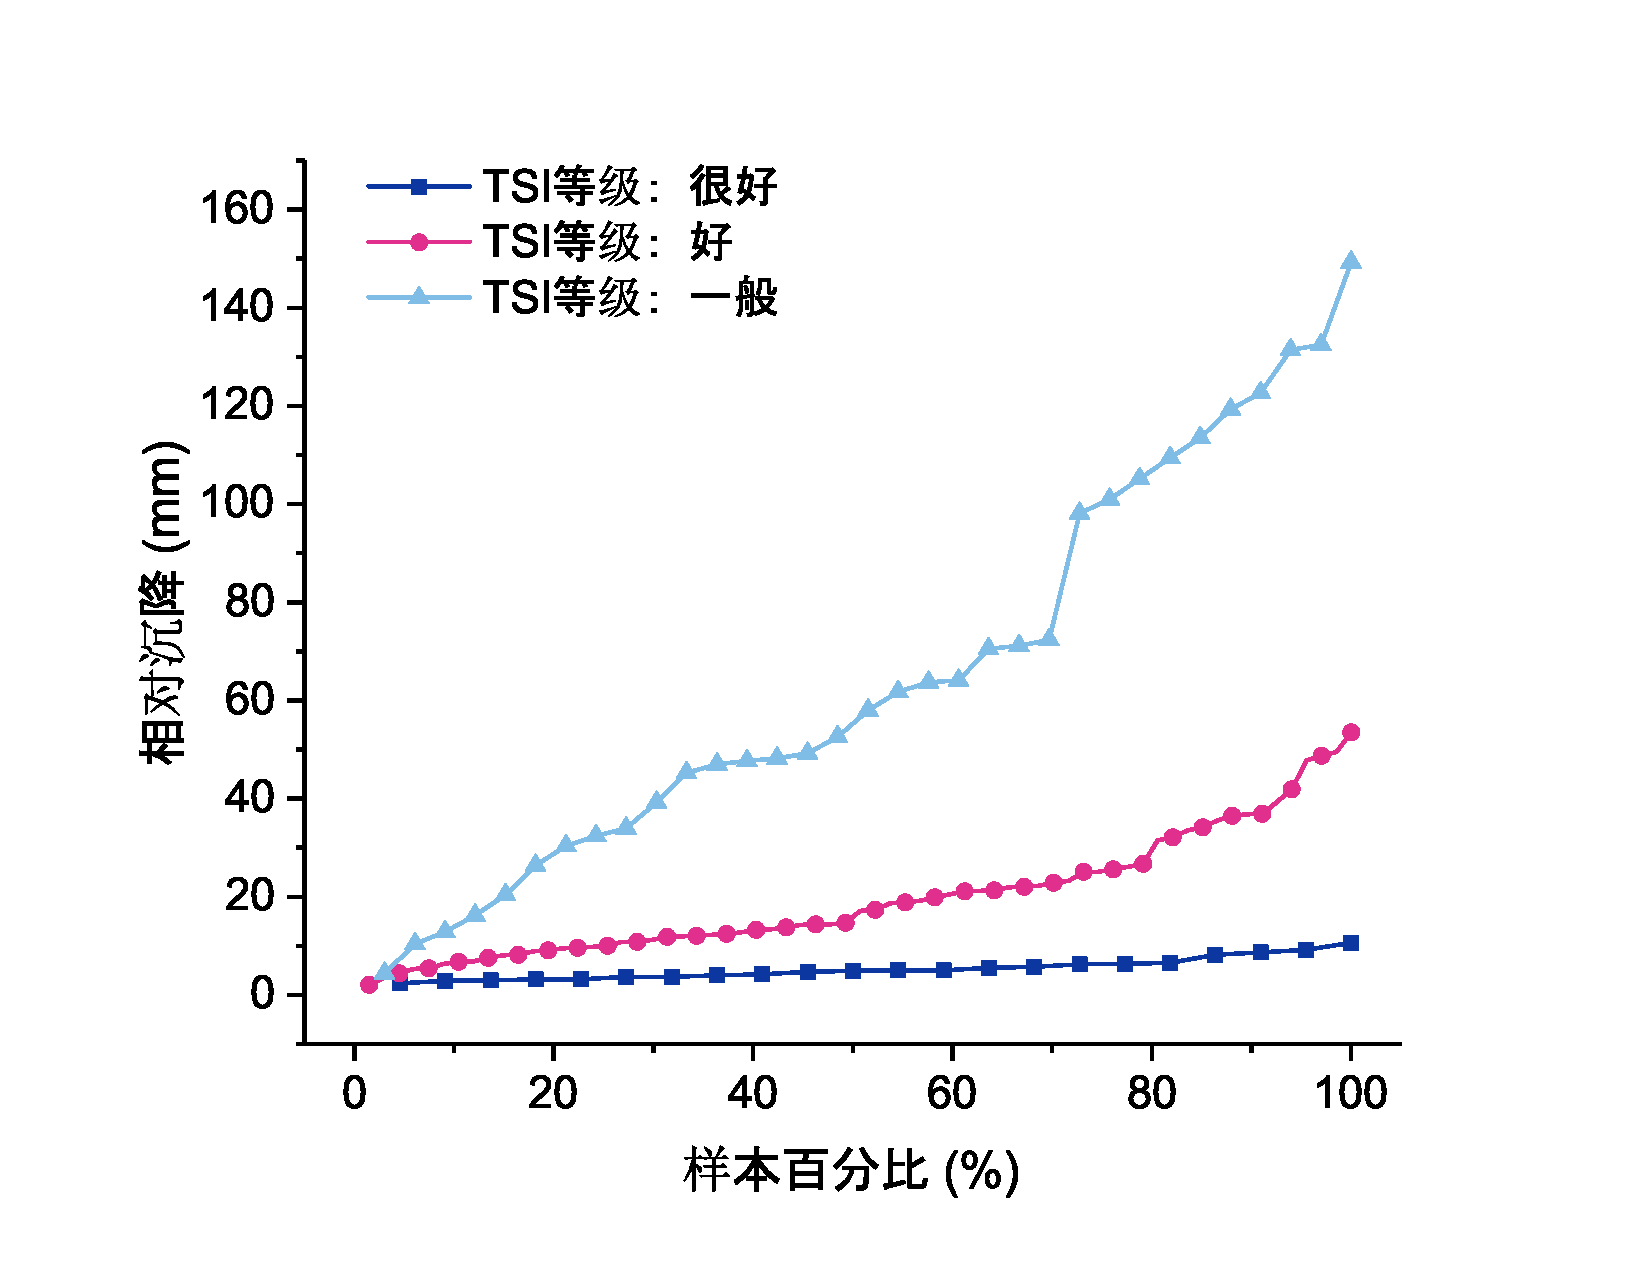
\includegraphics[width=0.57\textwidth]{chap2/tsi-statistics-sett.eps} \\ 
        (a)~相对沉降${sett}_{a}$统计 \\
        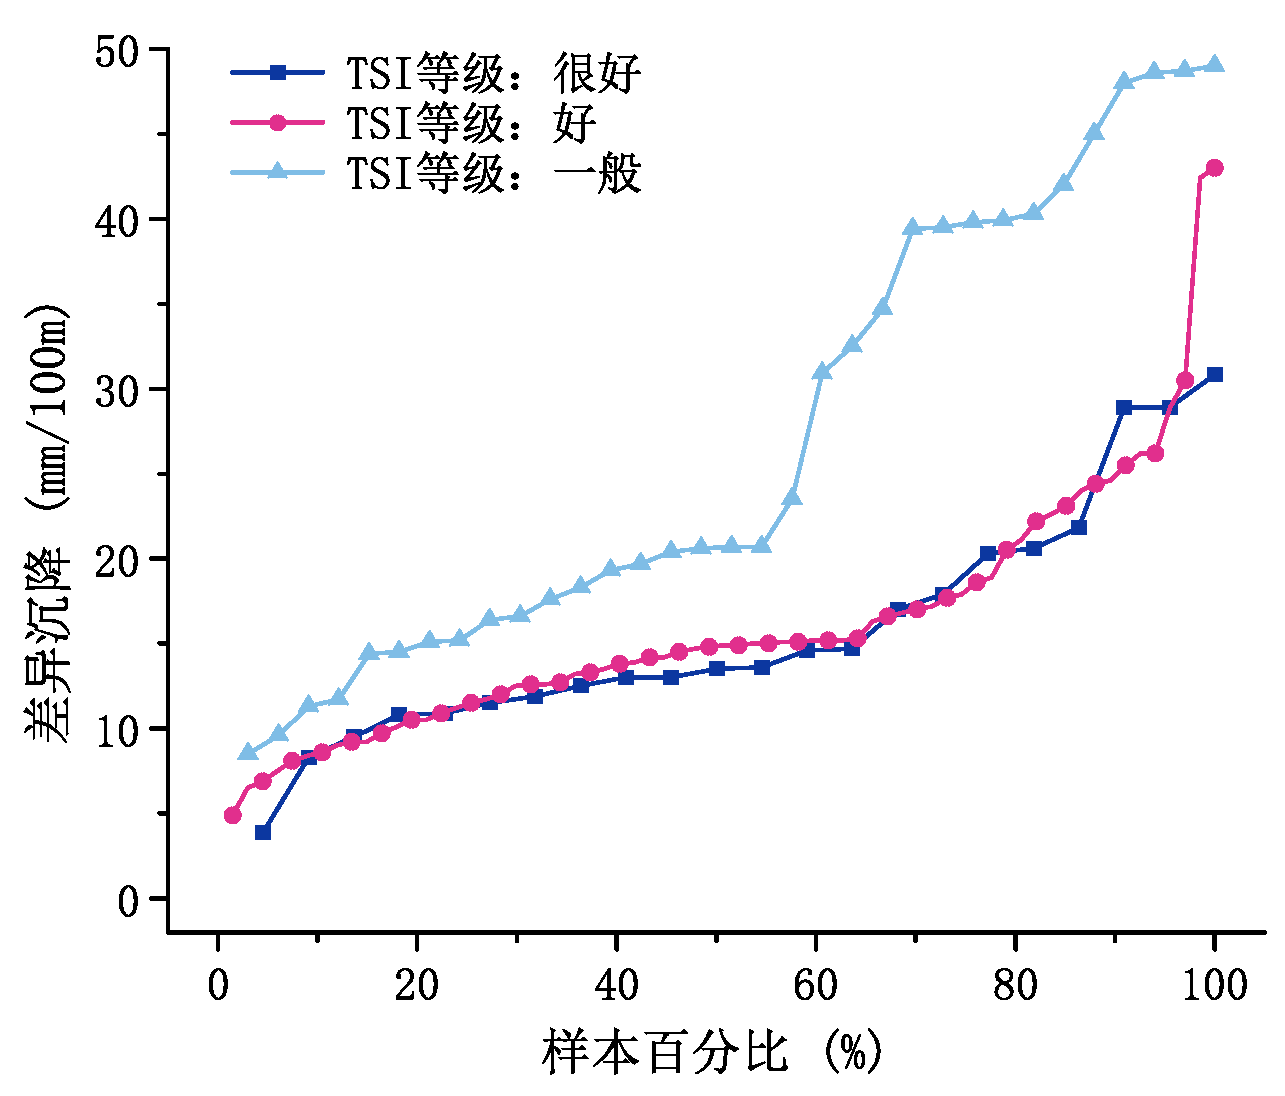
\includegraphics[width=0.57\textwidth]{chap2/tsi-statistics-settd.eps} \\ 
        (b)~差异沉降$set{{t}_{d\_a}}$统计 \\
        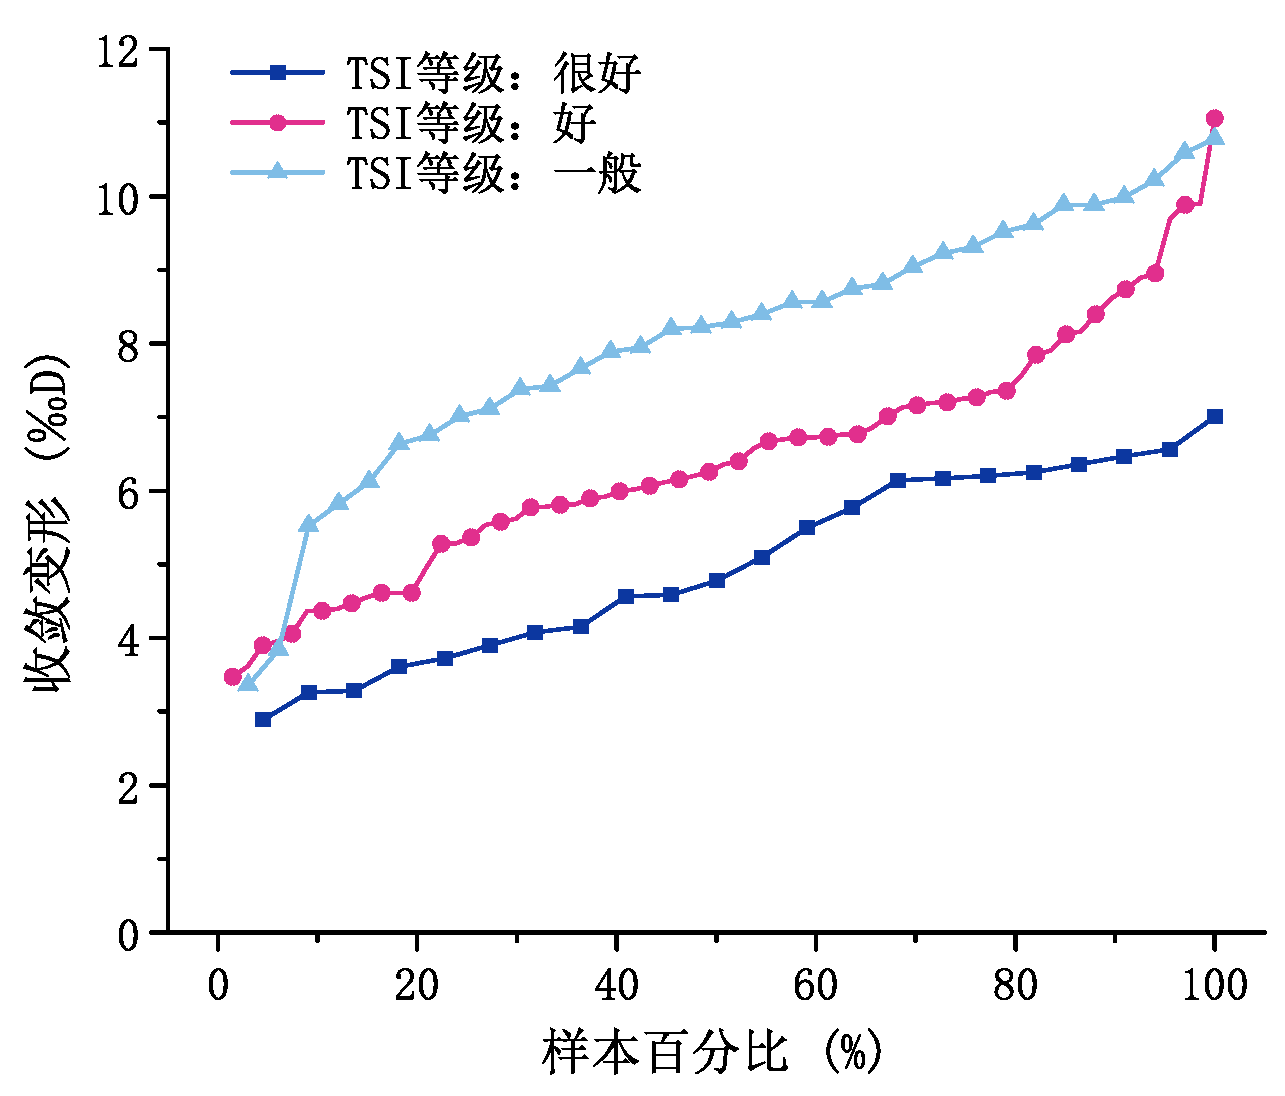
\includegraphics[width=0.57\textwidth]{chap2/tsi-statistics-cov.eps} \\ 
        (c)~收敛变形${cov}_{a}$统计 \\
    \end{tabular}
    \caption{上海地铁隧道TSI评估结果统计} 
    \label{fig:上海地铁隧道TSI评估结果统计} 
\end{figure}

\begin{figure}[htbp!] 
    \centering 
    \begin{tabular}{c} 
        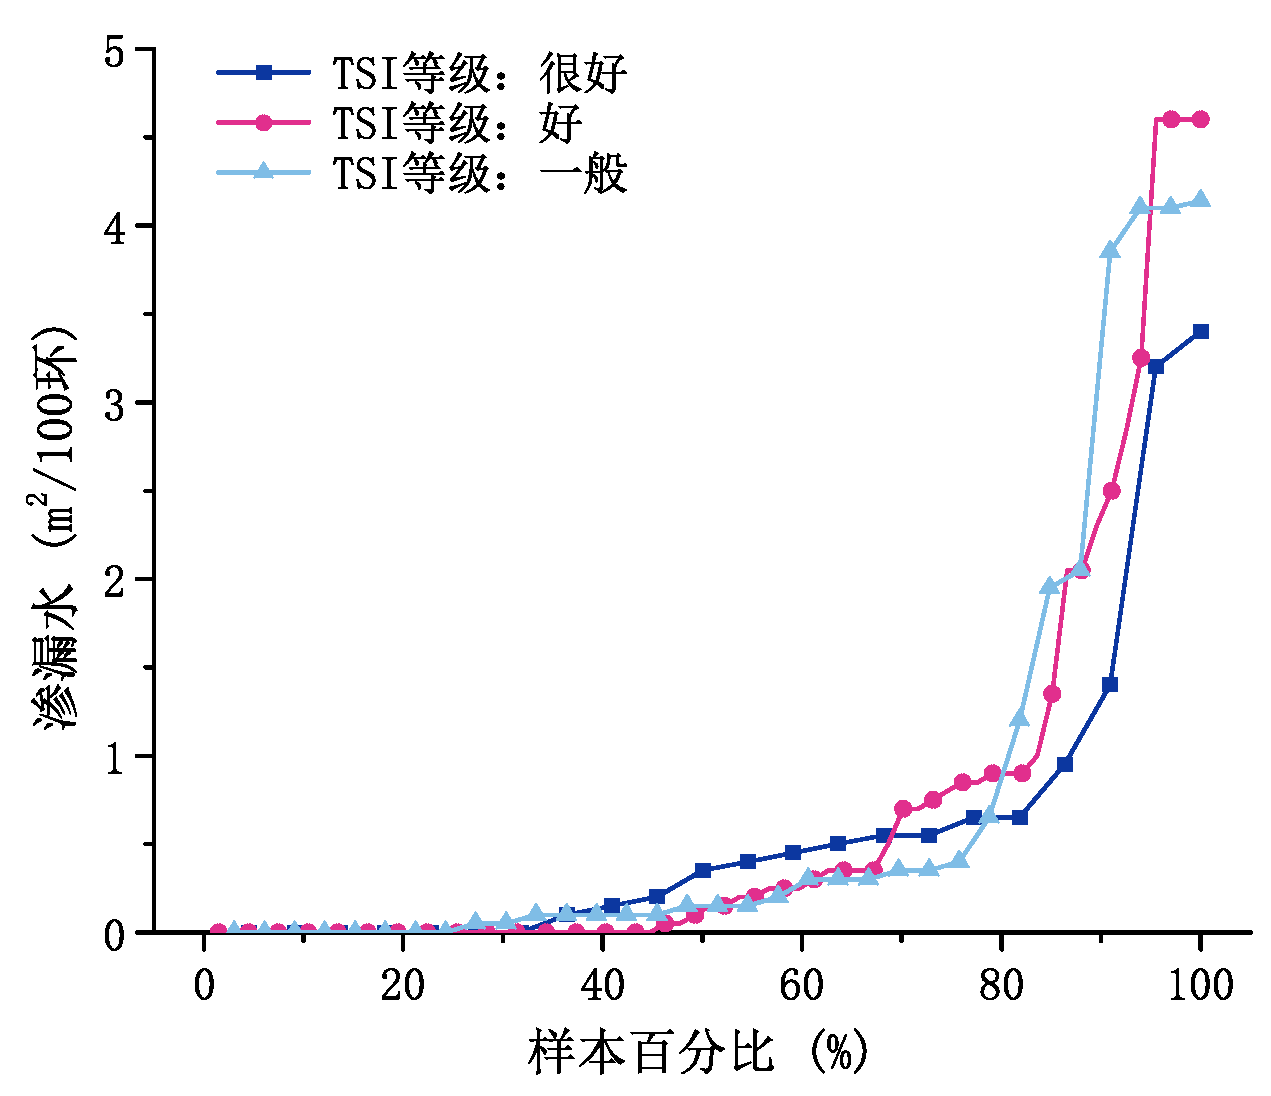
\includegraphics[width=0.57\textwidth]{chap2/tsi-statistics-leakage.eps} \\ 
        (a)~渗漏水$d_l$统计 \\
        \includegraphics[width=0.57\textwidth]{chap2/tsi-statistics-crack.eps} \\ 
        (b)~裂缝$d_c$统计 \\
        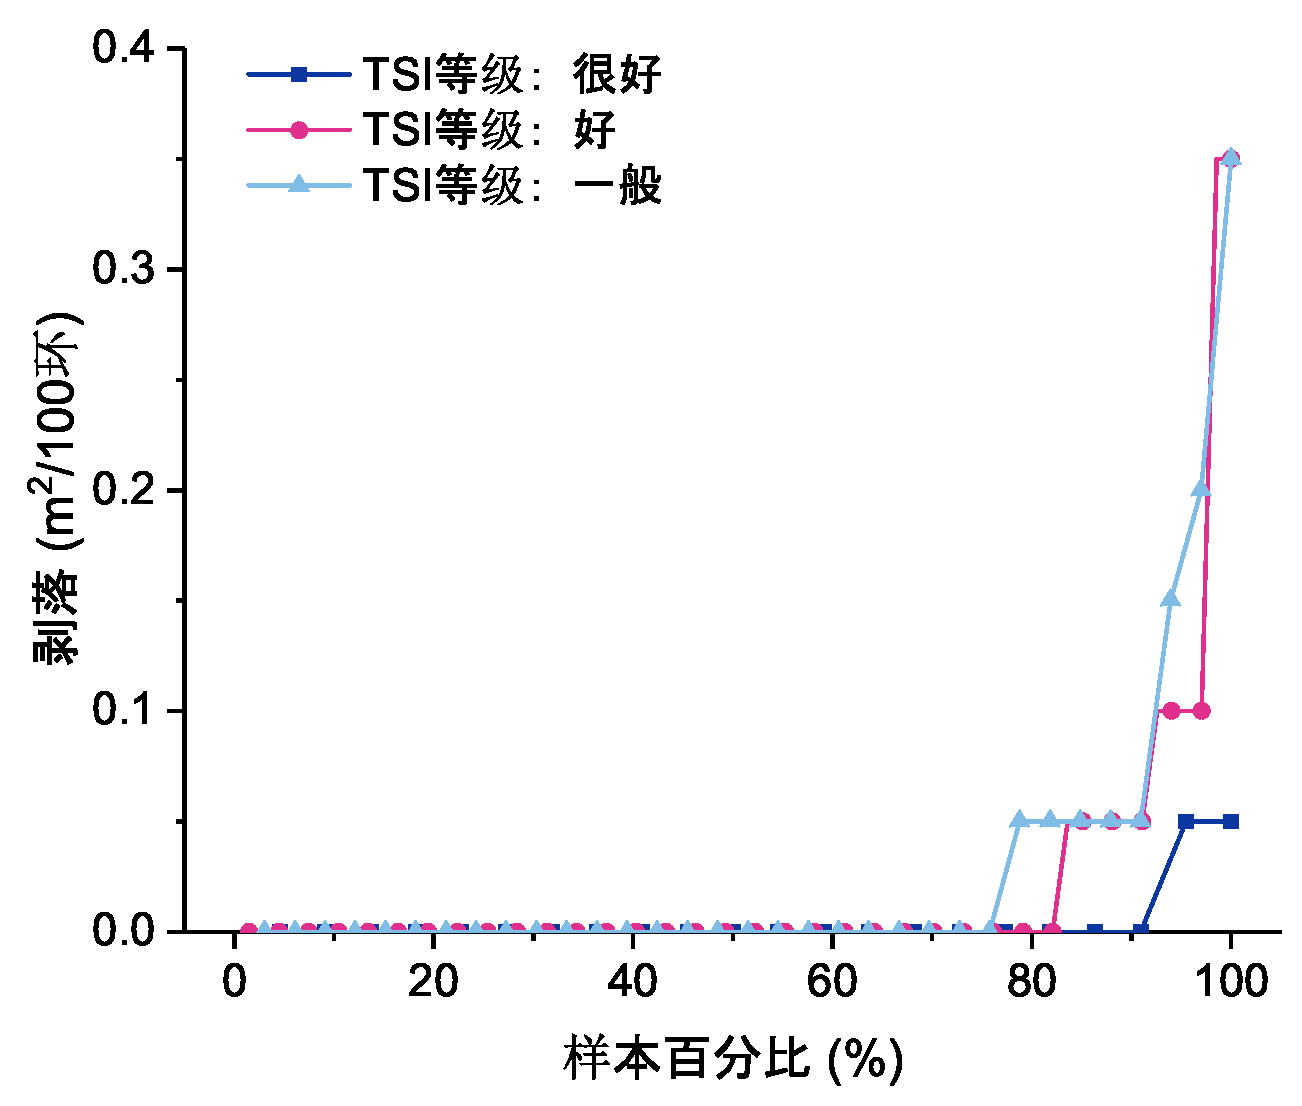
\includegraphics[width=0.57\textwidth]{chap2/tsi-statistics-spall.eps} \\ 
        (c)~剥落$d_s$统计 \\
    \end{tabular}
    \caption{上海地铁隧道TSI评估结果统计} 
    \label{fig:上海地铁隧道TSI评估结果统计2} 
\end{figure}

\begin{figure}[htbp!] 
    \centering 
    \begin{tabular}{c}
        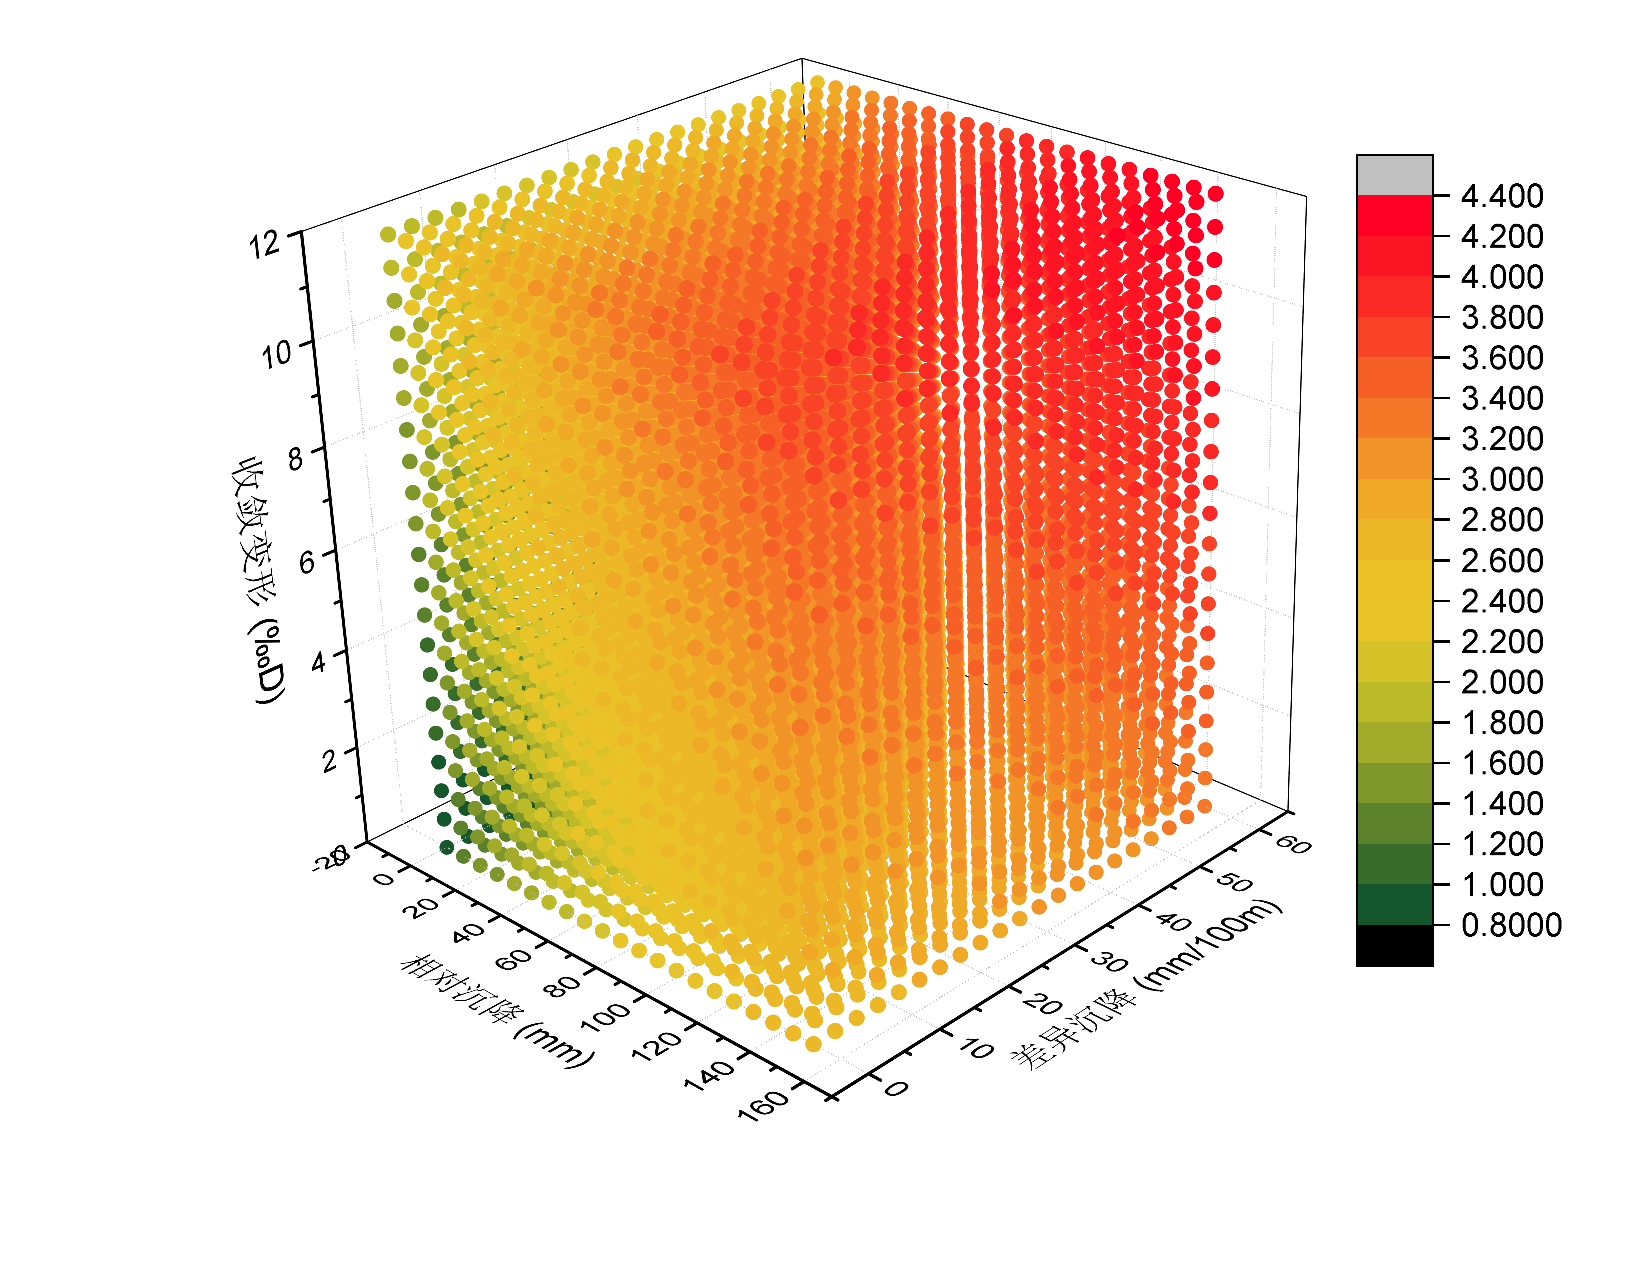
\includegraphics[width=1.0\textwidth]{chap2/triangle-except-leakage.eps} \\ 
        (a)~${sett}_{a}$-$set{{t}_{d\_a}}$-$cov_a$ \\
        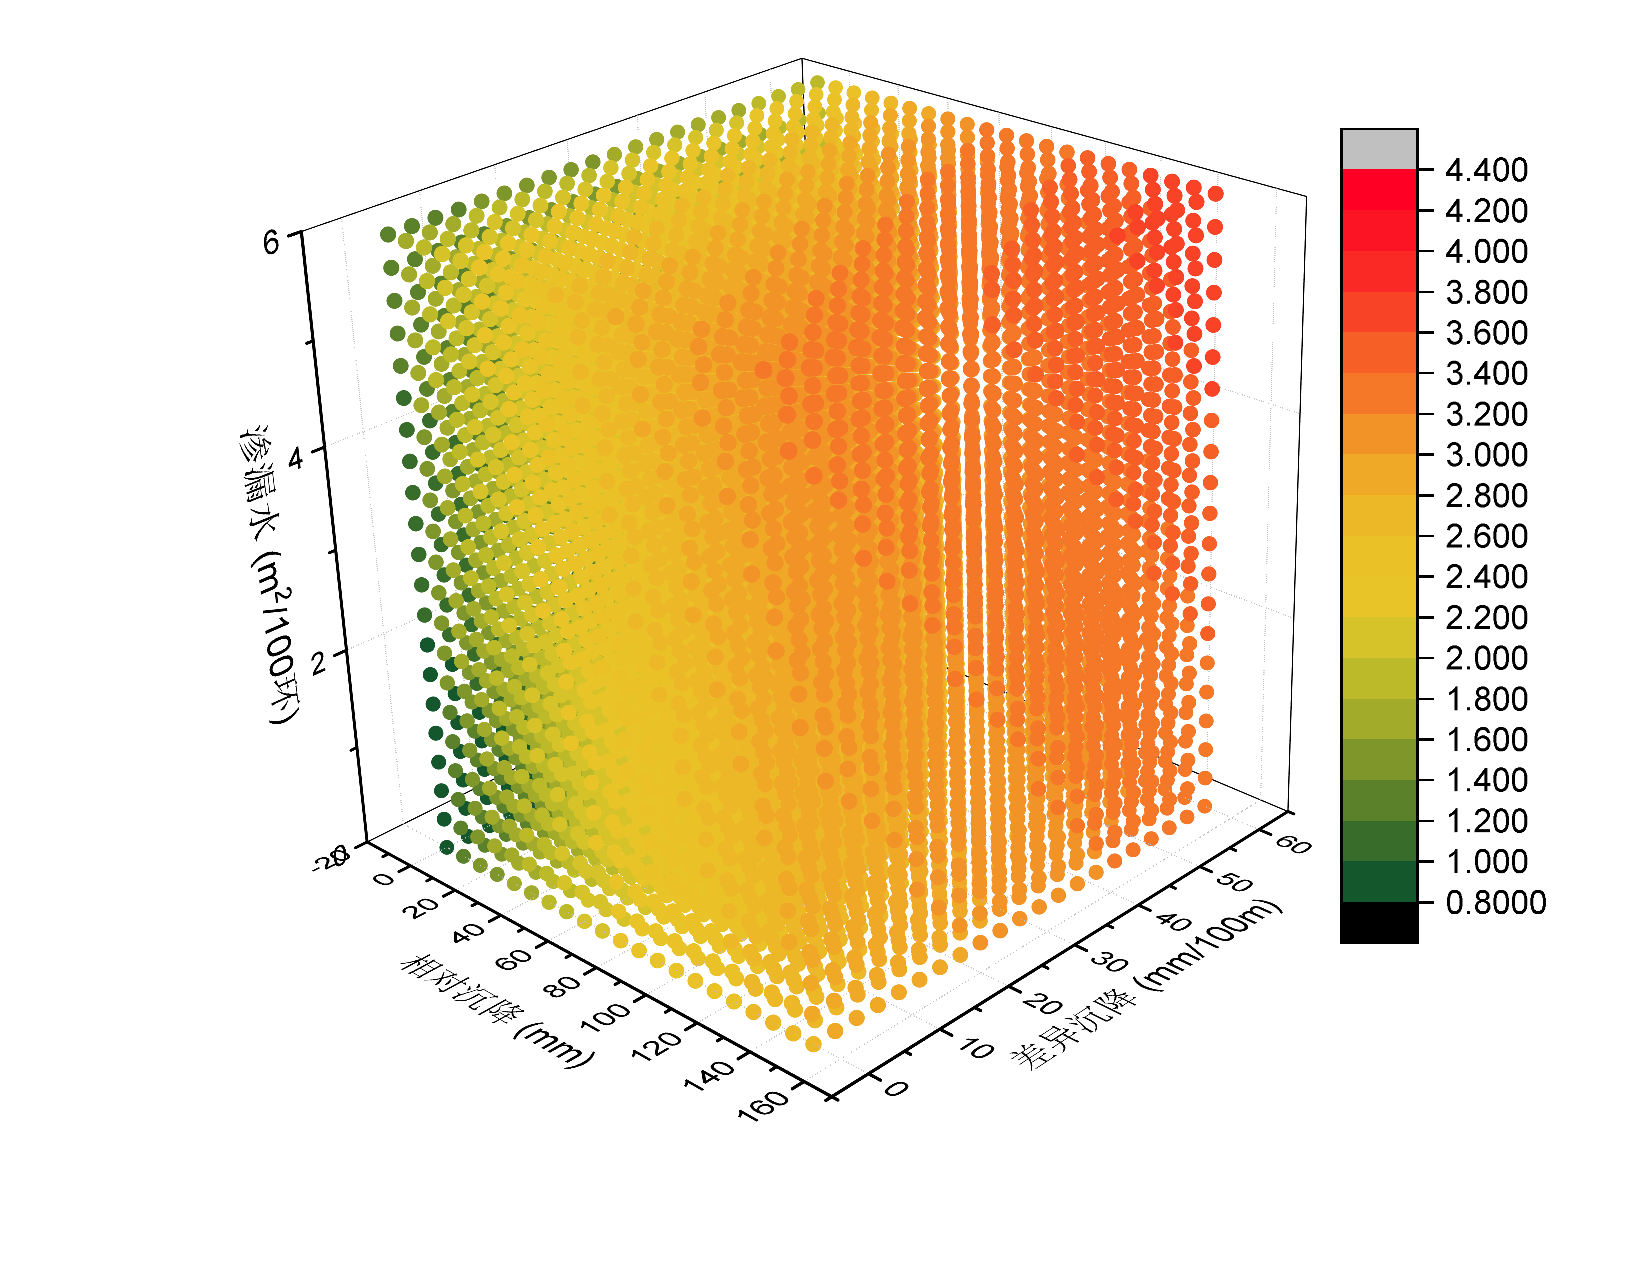
\includegraphics[width=1.0\textwidth]{chap2/triangle-except-conv.eps} \\ 
        (b)~${sett}_{a}$-$set{{t}_{d\_a}}$-$d_l$ \\
    \end{tabular}
    \caption{评估指标数值与TSI结果关系} 
    \label{fig:评估指标数值与TSI结果关系} 
\end{figure}

\begin{figure}[htbp!] 
    \centering 
    \begin{tabular}{c}
        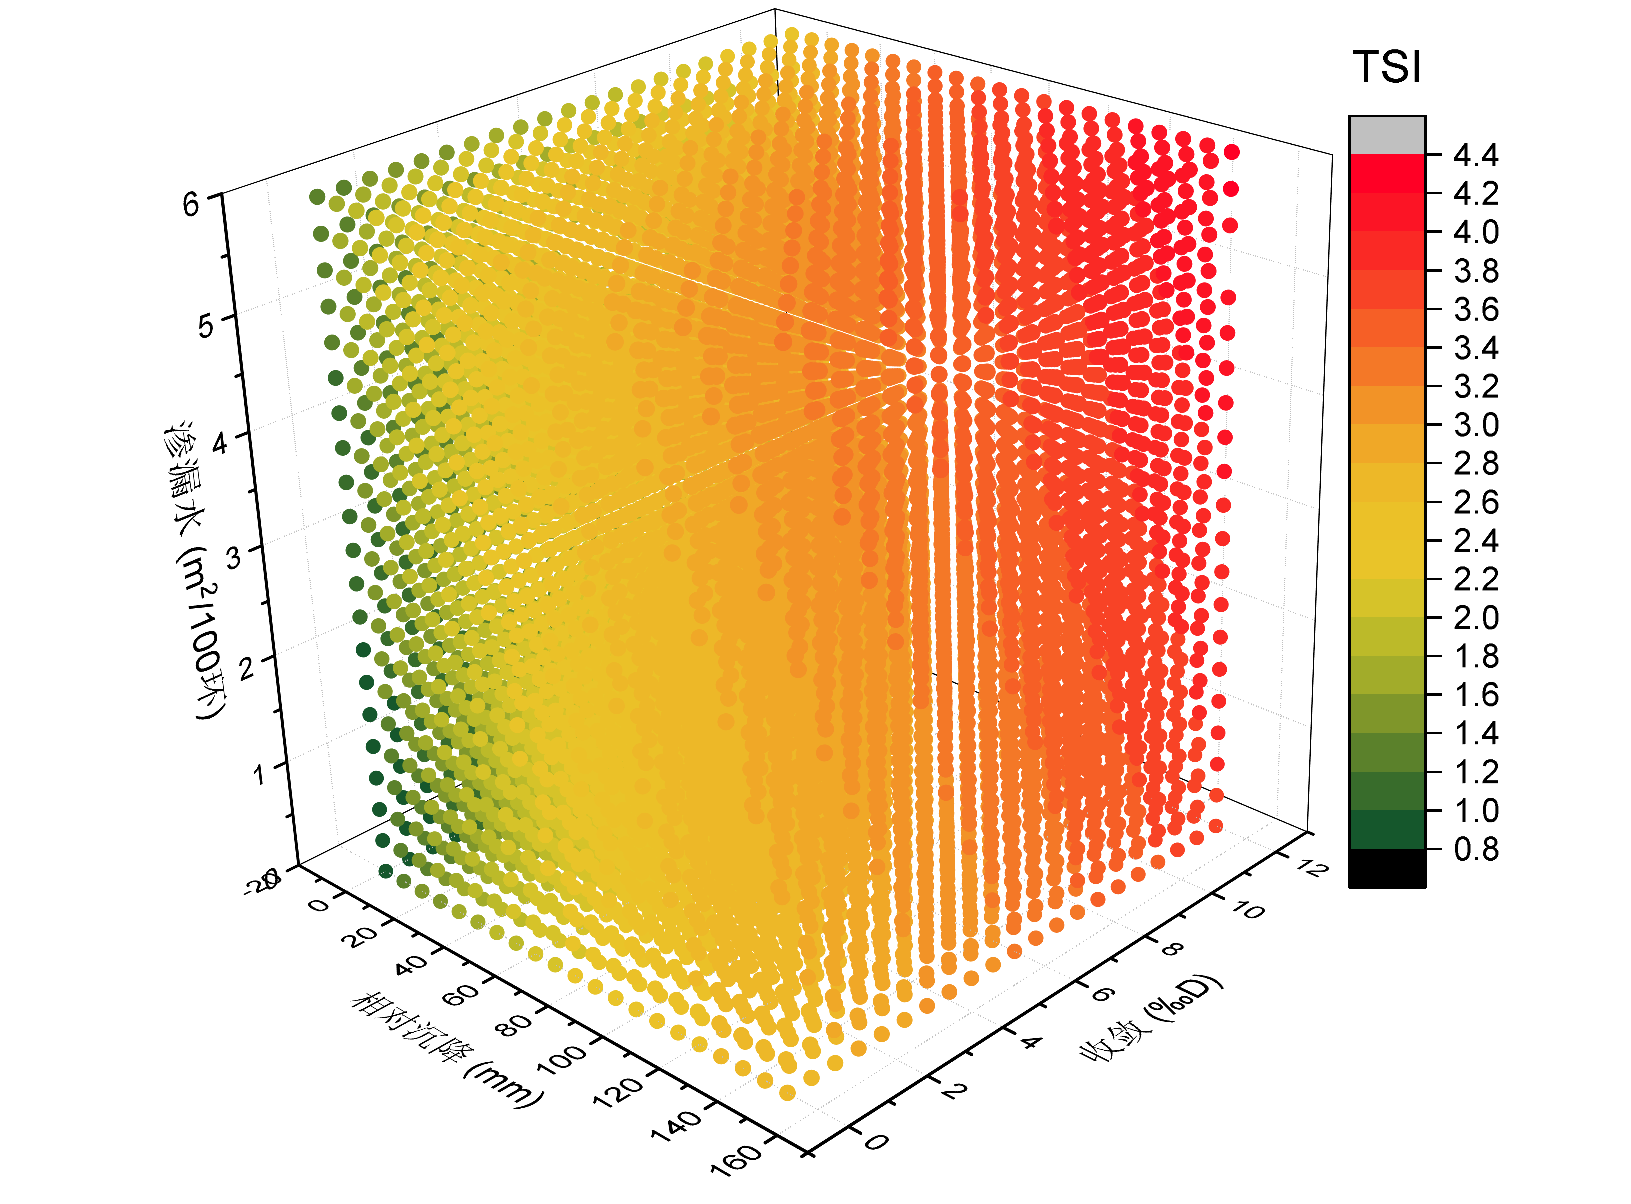
\includegraphics[width=1.0\textwidth]{chap2/triangle-except-settd.eps} \\ 
        (a)~${sett}_{a}$-$cov_a$-$d_l$ \\
        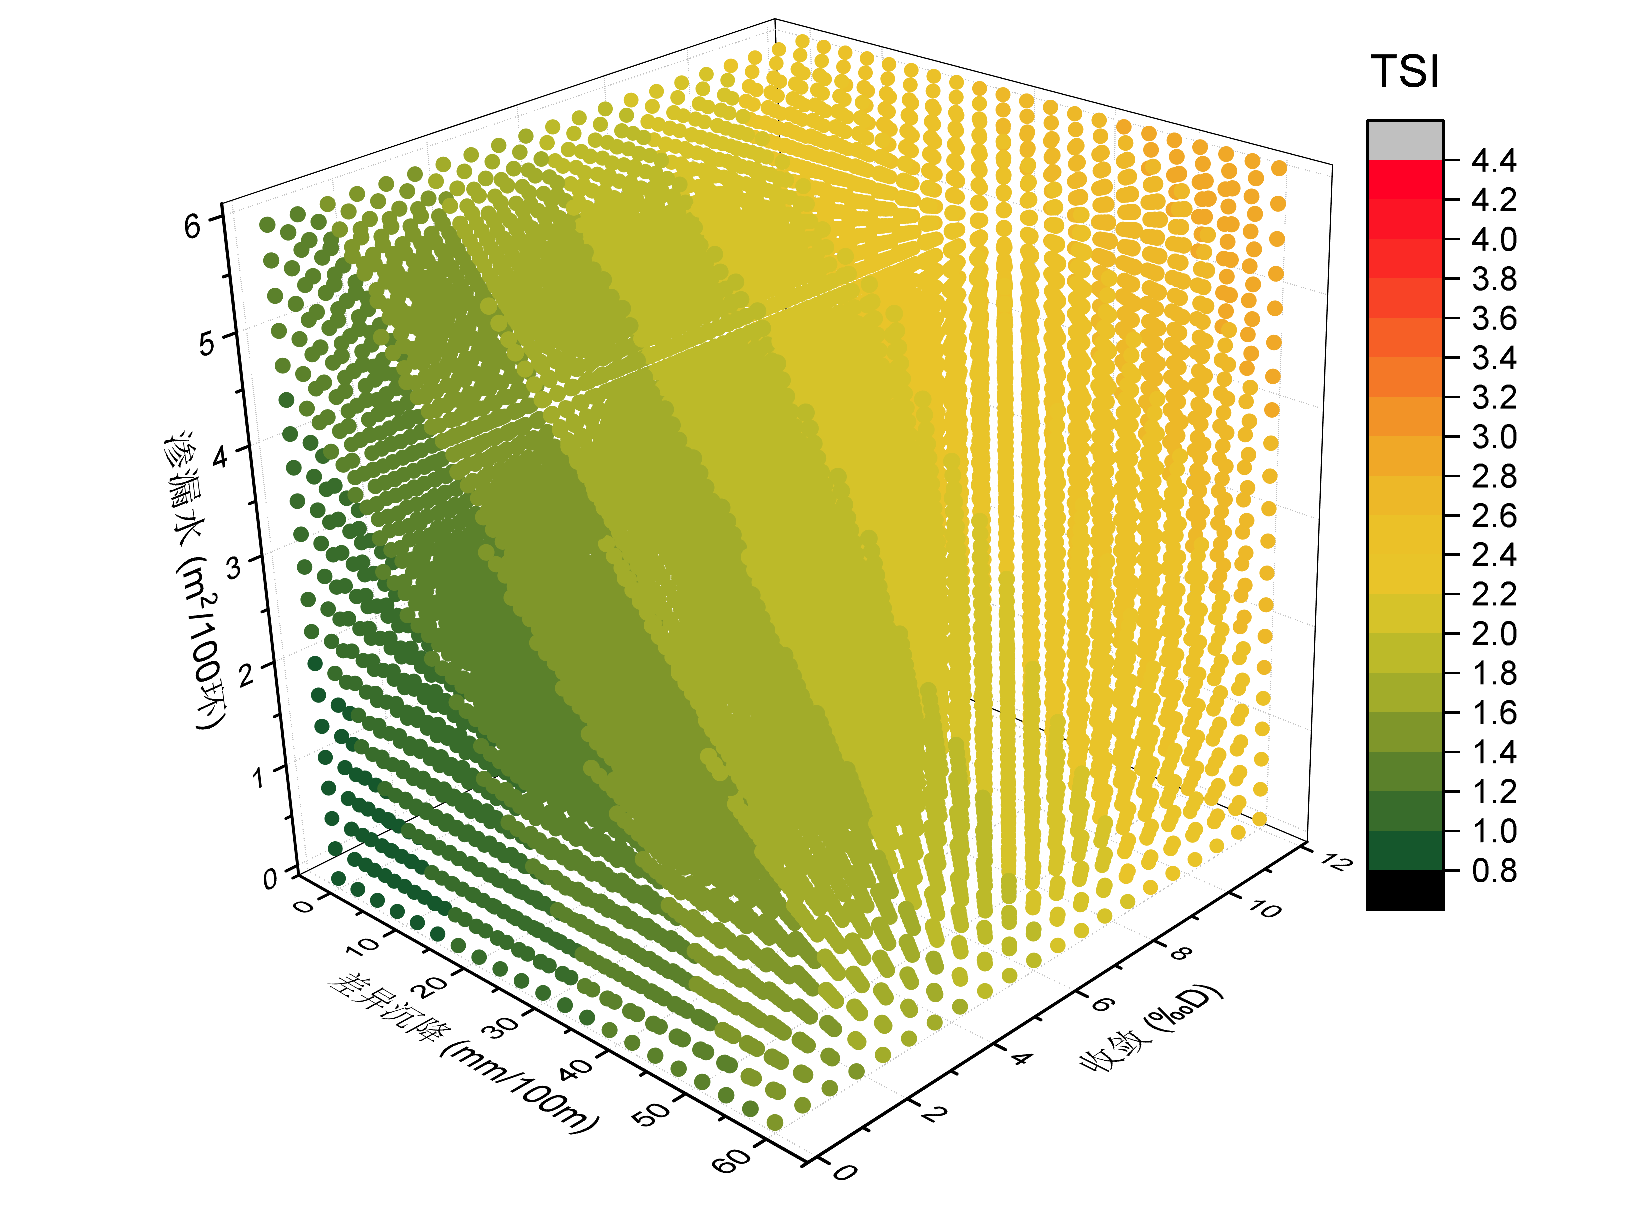
\includegraphics[width=1.0\textwidth]{chap2/triangle-except-sett.eps} \\ 
        (b)~$set{{t}_{d\_a}}$-$cov_a$-$d_l$ \\
    \end{tabular}
    \caption{评估指标数值与TSI结果关系} 
    \label{fig:评估指标数值与TSI结果关系2} 
\end{figure}

%%%%%%%%%%%%%%%%%%%%%%%%%%%%%%%%%%%%%%%%%%%%%%%%%%%%%%%%%%%%%%%%%%%
\section{TSI指标全寿命期修正}

公式~\ref{tsi}~给出了TSI与评估指标之间的关系,受限于当前隧道样本数量,TSI公式存在以下两个适用条件:(1)目前隧道区间样本的运营时间均在20年以内,对比100年的设计寿命,隧道仍处于早期阶段,对于20年以后的隧道服役性能,公式~\ref{tsi}~并不能模拟;(2)TSI公式严格上只适用于与样本类似的隧道区间,即统计指标如表~\ref{tab:上海地铁观测变量统计信息}~,若因外部因素导致评估指标远离统计范围,TSI公式也将不适用。

因此,本文研究了指标的劣化对服役性能的影响。本节采用动态变权的思想,对TSI公式在隧道全寿命期应用进行修正。动态变权函数应具备如下特点:(1)当各评估在表~\ref{tab:上海地铁观测变量统计信息}~统计范围内时,变权计算结果应与常权计算结果相近;(2)指标劣化程度越大,权重应越大,且权重增加的速率应正比于指标劣化程度,凸显指标对服役性能的影响;(3)当指标超过理论的极限值后,服役性能指标应能降至最低等级。建议在实际应用中,条件允许情况下均使用修正后的公式,未修正的TSI公式可用于简单估算。

动态变权首先需要考虑指标的劣化程度。以盾构隧道的累积沉降为例,在相同时间内新增相同的沉降,对累积沉降已经较大的隧道的影响要比累积沉降相对较小的隧道,数学上称这种特性为悲观性(李蓉,\citeyear{李蓉2007基于层次分析法的桥梁健康状态模糊综合评估方法的研究及其应用}),其数学公式为
\begin{equation}
    g=G(v)=\left\{ \begin{matrix}
   1-\left( \frac{v-{{v}_{\min }}}{{{v}_{\max }}-{{v}_{\min }}} \right){{e}^{\frac{v-{{v}_{\min }}}{{{v}_{\max }}-{{v}_{\min }}}-1}}\quad {{v}_{\max }}\ge v\ge {{v}_{\min }}  \\
   0\quad \quad \quad \quad \quad \quad \quad v>{{v}_{\max }}  \\
\end{matrix} \right.
\end{equation}
式中:$g$为指标健康度,$g$越小代表指标越严重;$v$为指标的值;$v_{min}$为指标的下限值;$v_{max}$为指标的上限值。曲线如图~\ref{fig:悲观型曲线图}~所示。

\begin{figure}[htb!]
    \centering
    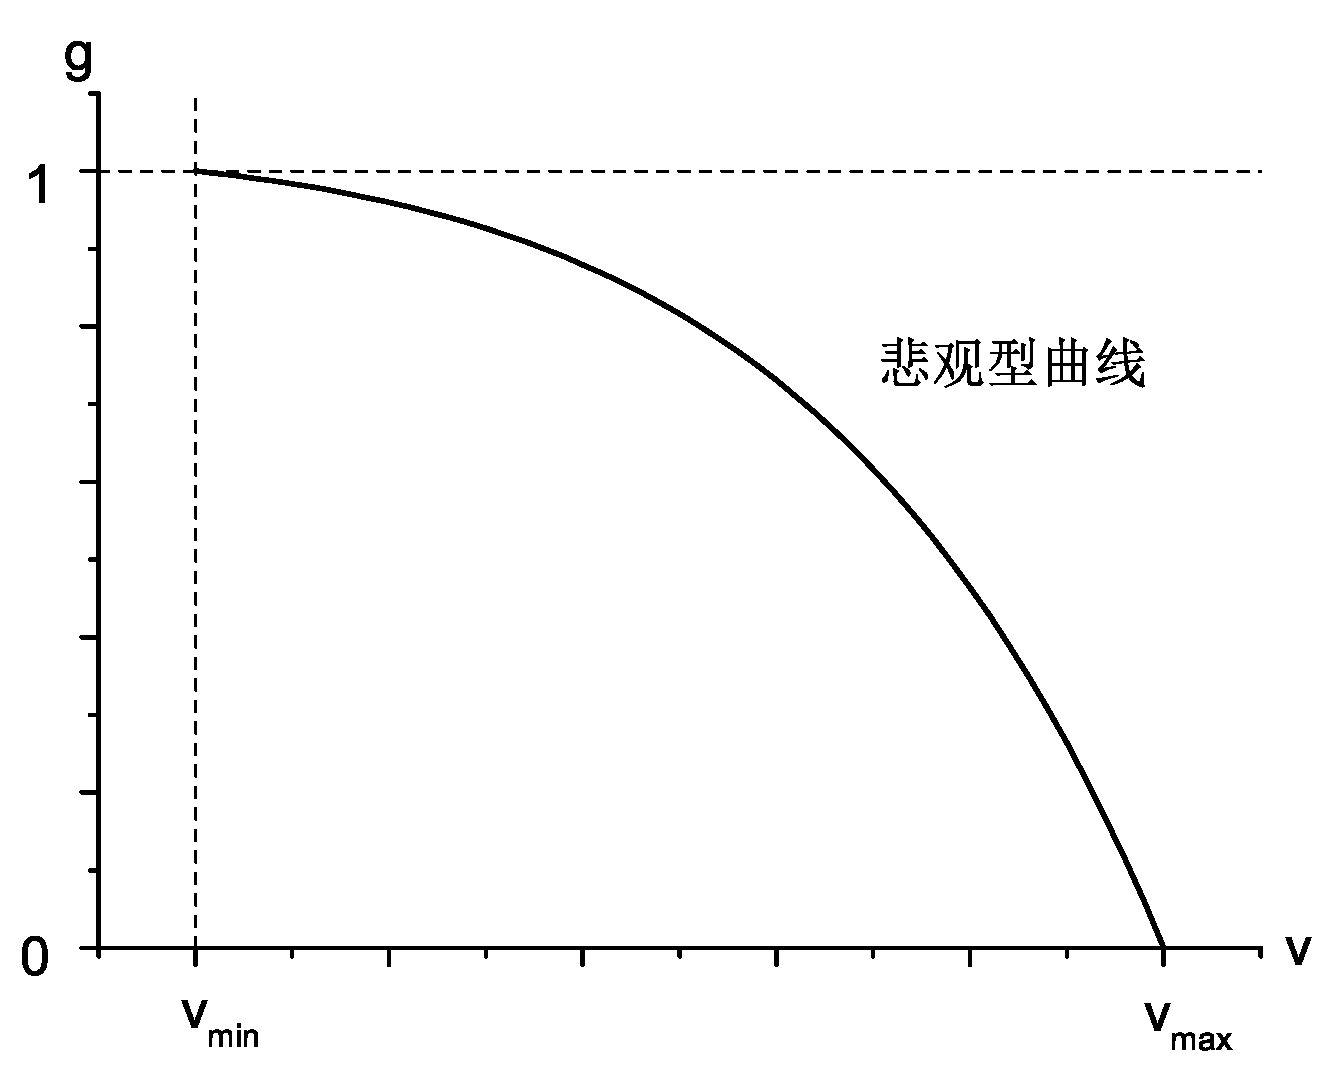
\includegraphics[width=0.7\textwidth]{chap2/stdline.eps}
    \caption{悲观型曲线图}
    \label{fig:悲观型曲线图}
\end{figure}

Cheng等(\citeyear{cheng1999evaluating})引入变权函数,采用变权权重替换常权权重,反映指标不同劣化程度在TSI计算时的重要程度不同。对于变权和状态函数的公理化定义如下:

定义一:一组变权$\mathbf{{w}'}(\mathbf{g})=\left( {{{{w}'}}_{1}}(\mathbf{g}),{{{{w}'}}_{2}}(\mathbf{g}),\cdots ,{{{{w}'}}_{n}}(\mathbf{g}) \right)$,指的是对应$n$个指标的映射${{{w}'}_{i}}(i=1,2,\cdots ,n)$,${{{w}'}_{i}}:({{g}_{1}},{{g}_{2}},\cdots ,{{g}_{n}})\mapsto {{{w}'}_{i}}({{g}_{1}},{{g}_{2}},\cdots ,{{g}_{n}})$,应满足:

(1)归一性:$\sum\limits_{i=1}^{n}{{{{{w}'}}_{i}}({{g}_{1}},\cdots ,{{g}_{n}})=1}$;

(2)连续性:${{{w}'}_{i}}({{g}_{1}},\cdots ,{{g}_{n}})(i=1,\cdots ,n)$对所有变元$g_i$是连续的;

(3)惩罚性:${{{w}'}_{i}}({{g}_{1}},\cdots ,{{g}_{n}})(i=1,\cdots ,n)$对所有变元$g_i$是单调下降的;

(3$'$)激励性:${{{w}'}_{i}}({{g}_{1}},\cdots ,{{g}_{n}})(i=1,\cdots ,n)$对所有变元$g_i$是单调上升的;

(3$''$)混合性:${{{w}'}_{i}}({{g}_{1}},\cdots ,{{g}_{n}})(i=1,\cdots ,n)$对部分变元单调下降,对部分变元单调上升。

定义二:映射$\mathbf{g}\mapsto \mathbf{d}(\mathbf{g})=({{d}_{1}}(\mathbf{g}),\cdots ,{{d}_{n}}(\mathbf{g}))$,称$\mathbf{d}(\mathbf{g})$为一个$n$维变权向量,${d}(\mathbf{g})$为状态变权函数,其满足

(1)惩罚型:${{g}_{i}}\ge {{g}_{j}}\Rightarrow {{d}_{i}}(\mathbf{g})\le {{d}_{j}}(\mathbf{g})$;

(1$'$)激励型:${{g}_{i}}\ge {{g}_{j}}\Rightarrow {{d}_{i}}(\mathbf{g})\ge {{d}_{j}}(\mathbf{g})$;

(2)${{d}_{i}}(\mathbf{g})(i=1,\cdots .n)$对所有变元$g_i$连续;

(3)对常权向量$\mathbf{w}=({{w}_{1}},\cdots ,{{w}_{n}})$,可构造变权公式
\begin{equation}
    \label{equ:状态变权函数}
    \mathbf{{w}'}(\mathbf{g})=\frac{({{w}_{1}}{{d}_{1}}(\mathbf{g}),\cdots ,{{w}_{n}}{{d}_{n}}(\mathbf{g})}{\sum\limits_{i=1}^{n}{({{w}_{i}}{{d}_{i}}(\mathbf{g}))}}=\frac{\mathbf{w}\cdot \mathbf{d}(\mathbf{g})}{\sum\limits_{i=1}^{n}{({{w}_{i}}{{d}_{i}}(\mathbf{g}))}}
\end{equation}

公式~\ref{equ:状态变权函数}~最重要的是选择合适的状态变权函数,在数学上,常用的函数为幂函数形式(孙九春,\citeyear{孙九春2002大型桥梁综合评估系统研究}),如式~\ref{equ:幂函数变权函数}
\begin{equation}
    \label{equ:幂函数变权函数}
    {{d}_{i}}(\mathbf{g})={{(\frac{{{g}_{i}}}{100})}^{\varepsilon -1}}\quad 0<\varepsilon <1
\end{equation}

采用幂函数作为状态变权函数时,只有当指标接近指标上限时,权重变化才明显,变权灵敏度在指标发展前期仍然较低。而且式~\ref{equ:幂函数变权函数}~在$g=0$时奇异,也给计算带来不便。对于盾构隧道的实际情况,陈楠(\citeyear{陈楠2017考虑发展趋势与指标关联的隧道结构健康评估方法研究})提出采用分段状态变权函数替代幂函数
\begin{equation}
    \label{equ:分段状态变权函数}
    {{d}_{i}}(\mathbf{g})=\left\{ \begin{array}{*{35}{l}}
   {{m}^{4-5g}},0\le g\le 0.8  \\
   1,0.8 < g  \\
\end{array} \right.
\end{equation}
式中:$m$为形状参数,一般可取$m=2.5$。

图~\ref{fig:分段变权函数与幂函数变权函数比较}~描述了分段状态变权函数与幂函数状态变权函数的形状,由图可知,当某一指标的健康度$g$降低至0.8时,该指标所占权重将略微有所增加,当$g$继续降低至0.6-0.4时,所占权重将会有明显的增加,当$g$降低至0.2时,也就是一般单项指标预警值临界值时,指标权重将迅速增加,使该指标起决定作用。分段状态变权与幂函数变权公式相比,在指标发展早期有较好的预警效果。

\begin{figure}[htbp]
    \centering
    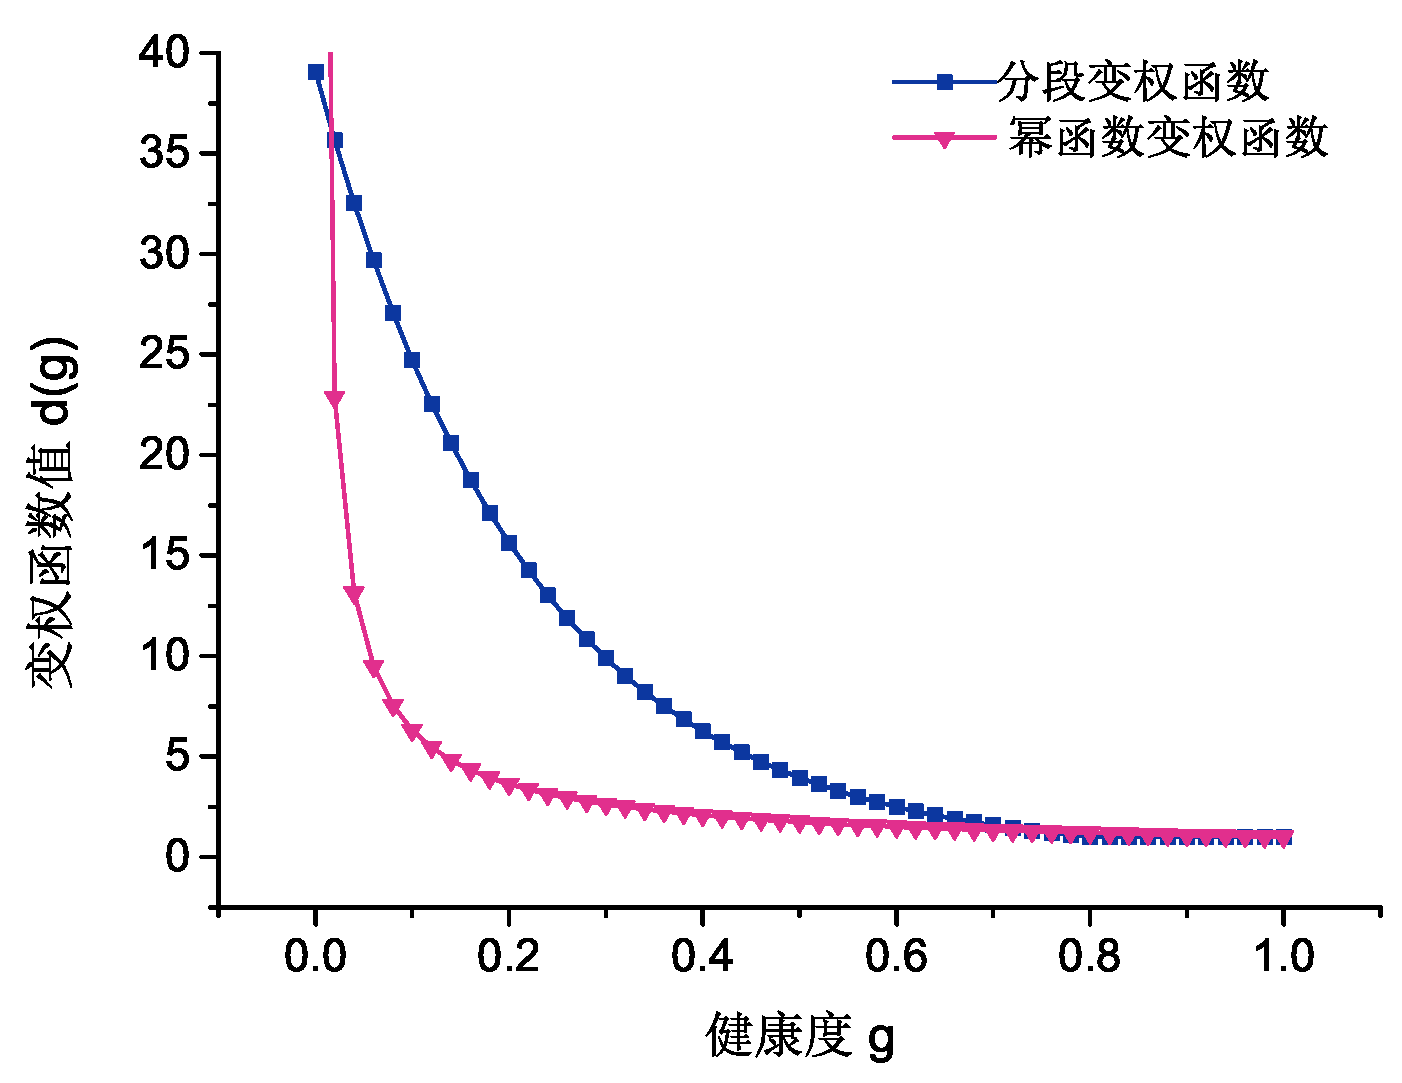
\includegraphics[width=0.7\textwidth]{chap2/dynamic-weight.eps}
    \caption{分段变权函数与幂函数变权函数比较}
    \label{fig:分段变权函数与幂函数变权函数比较}
\end{figure}

%%%%%%%%%%%%%%%%%%%%%%%%%%%%%%%%%%%%%%%%%%%%%%%%%%%%%%%%%%%%%%%%%%%
\section{空间网格化TSI指标评估}

\subsection{空间变异结构与变异函数}

盾构隧道服役性能指标计算的是某一段区间的TSI值,对于地铁的网状结构,可计算得出空间上不同位置的TSI值,服役性能在空间上不一定是完全随机的或完全独立的,可能存在相互联系。统计上可用变异函数来表征变量的空间变异结构,或空间连续性。

网格化变量在某方向上相距$h$的增量的方差,称为网格化变量在该方向上的变异函数
\begin{equation}
    2\gamma (h)\text{=E}\left\{ {{\left[ \text{Z(x+h)-Z(x)} \right]}^{2}} \right\}
\end{equation}
式中:$\gamma (h)$为(半)变异函数;$Z(x)$为随机函数;$h$为距离。

以$\gamma (h)$为纵轴,$h$为横轴绘制$\gamma (h)$随滞后增加的变化曲线称为变异函数图,在实际应用中发现变异函数是滞后的单调函数,随着$h$由小增大,$\gamma (h)$逐渐增加,当$h$增大到某一数值时(变程),$\gamma (h)$增加到最大值(阈值),超过变程距离的变量,认为空间上自相关性为0。

已被证明有效的、常用的变异函数模型有(Rubin,\citeyear{rubin2003applied}):(1)球型模型
\begin{align}
& \gamma (h)=\left\{ \begin{array}{*{35}{l}}
   {{C}_{0}}+{{C}_{1}}\left[ 1.5(h/a)-0.5{{(h/a)}^{3}} \right],0\le h\le a  \\
   {{C}_{0}}+{{C}_{1}},h>a  \\
\end{array} \right.
\end{align}
式中:$C_0$为块金值;$C_0+C_1$为基台值;$a$为变程。

(2)指数模型
\begin{equation}
    \gamma (h)={{C}_{0}}+{{C}_{1}}(1-{{e}^{-h/a}})
\end{equation}

(3)高斯模型等
\begin{equation}
    \gamma (h)\text{=}{{C}_{0}}+{{C}_{1}}\left[ 1-{{e}^{-{{(h/a)}^{2}}}} \right]
\end{equation}

\subsection{克里金估计原理}

普通克里金方法要求变量满足固有假定的条件(Cressie,\citeyear{cressie1988spatial}),对于所有的变量$x$和距离$h$:

(1)$E\left[ Z(x+h)-Z(x) \right]=0$;

(2)$Var\left[ Z(x+h)-Z(x) \right]=2\gamma (h)$;

普通克里金的估计公式为(张仁铎,\citeyear{张仁铎2005空间变异理论及应用})
\begin{equation}
    {{Z}^{*}}({{x}_{0}})=\sum\limits_{i=1}^{n}{{{\lambda }_{i}}Z({{x}_{i}})}
\end{equation}
式中:${Z}^{*}(x_0)$是在$x_0$位置的估计值;$Z(x_i)$是$x_i$位置的测量值;${\lambda }_{i}$为对应权重;$n$为估计过程的测量值个数。

为保证无偏估计,令$E\left[ {{Z}^{*}}-Z \right]=0$,可得
\begin{equation}
    \sum\limits_{i=1}^{n}{{{\lambda }_{i}}=1}
\end{equation}

且估计值误差的方差可简化为
\begin{equation}
    S=2\sum\limits_{i=1}^{n}{{{\lambda }_{i}}\gamma ({{x}_{i}}-{{x}_{0}})-\sum\limits_{i=1}^{n}{\sum\limits_{j=1}^{n}{{{\lambda }_{i}}{{\lambda }_{j}}\gamma ({{x}_{i}}-{{x}_{j}})}}}
\end{equation}

在求估计方差的极小值时引入拉格朗日乘数$\mu $
\begin{equation}
    S=2\sum\limits_{i=1}^{n}{{{\lambda }_{i}}\gamma ({{x}_{i}}-{{x}_{0}})-\sum\limits_{i=1}^{n}{\sum\limits_{j=1}^{n}{{{\lambda }_{i}}{{\lambda }_{j}}\gamma ({{x}_{i}}-{{x}_{j}})}}}-2\mu (\sum\limits_{i=1}^{n}{{{\lambda }_{i}}-1})
\end{equation}

使估计方差最小,可得
\begin{equation}
    \label{equ:kriging}
    \frac{\partial S}{\partial {{\lambda }_{1}}}=0,\frac{\partial S}{\partial {{\lambda }_{2}}}=0,\cdots ,\frac{\partial S}{\partial {{\lambda }_{n}}}=0
\end{equation}

求解式~\ref{equ:kriging}~即可得到所有的权重${{\lambda }_{1}},{{\lambda }_{2}},\cdots ,{{\lambda }_{n}}$。

%%%%%%%%%%%%%%%%%%%%%%%%%%%%%%%%%%%%%%%%%%%%%%%%%%%%%%%%%%%%%%%%%%%
\section{隧道服役性能指标的应用}

\subsection{常权TSI应用}

以上海地铁12号线天潼路站至国客中心站区间为例,说明TSI公式的应用。该区间长1449.6米,环宽1.2米,共计1208环,平面图如图~\ref{fig:天潼路-国客中心区间平面图}~所示。通过监测与人工检查方式获得该隧道区间沉降数据如图~\ref{fig:天潼路-国客中心区间监测数据}a~所示,相对沉降大小在0-9mm范围,收敛数据如图~\ref{fig:天潼路-国客中心区间监测数据}b~所示,收敛变形大小在0-10‰D范围。

\begin{figure}[htb!]
    \centering
    \includegraphics[width=1.0\textwidth]{chap2/subway1.png}
    \caption{天潼路-国客中心区间平面图}
    \label{fig:天潼路-国客中心区间平面图}
\end{figure}

\begin{figure}[htb!] 
    \centering 
    \begin{tabular}{c} 
        \includegraphics[width=1.0\textwidth]{chap2/subway2.png} \\ 
        (a)~沉降数据 \\
        \includegraphics[width=1.0\textwidth]{chap2/subway3.png} \\ 
        (b)~收敛数据 \\
    \end{tabular}
    \caption{天潼路-国客中心区间监测数据} 
    \label{fig:天潼路-国客中心区间监测数据} 
\end{figure}

区间总共有19处渗漏水,其中最大渗漏面积发生在第599环,为1.6$m^2$;总共有23处裂缝,其中最大裂缝发生在第852环,为1$m$长;以及有12处剥落,其中最大剥落发生在第102环,为0.1$m^2$。区间的病害展开图如图~\ref{fig:天潼路-国客中心区间病害数据}~所示。

\begin{figure}[htb!]
    \centering
    \includegraphics[width=1.0\textwidth]{chap2/subway4.png}
    \caption{天潼路-国客中心区间病害数据}
    \label{fig:天潼路-国客中心区间病害数据}
\end{figure}

将隧道以200环为单位划分,计算各指标的数值大小,将结果代入式~\ref{tsi}~得,第1-200环TSI为
\begin{align}
  & TSI=0.77+0.16\sqrt{{{sett}_{a}}}+0.01{{sett}_{d\_a}}+0.09{{cov}_{a}} \nonumber \\ 
 & \quad \quad \quad +0.08{{d}_{l}}+0.05{{d}_{c}}+0.50{{d}_{s}} \nonumber \\ 
 & \quad \quad =0.77+0.16\times \sqrt{8.479}+0.01\times 20.064+0.09\times 5.325 \nonumber \\ 
 & \quad \quad \quad +0.08\times 3.4+0.05\times 3.852+0.5\times 0.1 \nonumber \\ 
 & \quad \quad =2.4 \nonumber
\end{align}
以此类推,可计算整个隧道区间的TSI值如图~\ref{fig:天潼路-国客中心区间服役性能结果}~所示。由图可知,该区间的状态在1.8-2.4之间,接近于“好(2.0)”状态,相对应的维护养护措施可参考~\ref{chap:tsi-maintenance}~小节的建议。

\begin{figure}[htb!]
    \centering
    \includegraphics[width=1.0\textwidth]{chap2/subway5.png}
    \caption{天潼路-国客中心区间服役性能结果}
    \label{fig:天潼路-国客中心区间服役性能结果}
\end{figure}

\subsection{全寿命周期变权TSI应用}

继续以12号线数据为例,说明变权TSI计算过程。首先应确定各指标的允许最大值,采用朱宝林(\citeyear{朱宝林2014运营地铁盾构隧道状态评估及预测方法研究})对隧道病害分级的建议值,本文对六个评估指标的极限值取值如表~\ref{tab:评估指标允许最小和最大值}~所示。仍以图~\ref{fig:天潼路-国客中心区间服役性能结果}~中常权TSI为2.4的第1-200环区段隧道为例,其指标数值如表~\ref{tab:TSI变权函数计算过程}~第2列所示,根据公式~\ref{tsi-std}~可知TSI标准化公式的指标系数如第3列所示,根据系数计算各指标的权重,结果为第4列数据,根据指标数值计算指标的健康度,如第5列,根据公式~\ref{equ:分段状态变权函数}~得到变权函数值,如第6列,最后重新计算各指标的权重和标准化系数,分别如第7、8列所示。

根据公式~\ref{equ:setta标准化}-\ref{equ:ds标准化}~可计算得到各指标的标准化值分别为:-0.74、0.21、-0.35、1.17、3.72和1.00,根据更新后的指标系数,可计算标准化后的TSI
\begin{align}
  & {\xi }_{TSI}=0.31\sqrt{{\xi }_{sett_a}}+0.23{\xi }_{sett_{d\_a}}+0.16\operatorname{\xi }_{cov_a} \nonumber \\ 
 & \quad \quad \quad +0.36{\xi }_{d_l}+0.20{\xi }_{d_c}+0.01{\xi }_{d_s} \nonumber \\ 
 & \quad \quad =0.31\times (-0.74)+0.23\times 0.21+0.16\times (-0.35) \nonumber \\ 
 & \quad \quad \quad +0.36\times 1.17+0.20\times 3.72+0.01\times 1.0 \nonumber \\ 
 & \quad \quad =0.9 \nonumber
\end{align}
再根据公式~\ref{equ:tsi标准化}~可计算得变权后的TSI值
\begin{equation}
    TSI={\xi }_{TSI}\times 0.8+2.4=3.1 \nonumber
\end{equation}
较常权TSI计算结果2.4增加了0.7,变权TSI计算结果为3.1,评估状态在“一般”级别,主要原因是该区段的差异沉降、渗漏水和裂缝较大,健康度的计算结果在0.5以下,对应指标的权重增加,反映指标对服役性能影响增大。

\begin{table}[htb!]
  \centering
  \caption{评估指标允许最小和最大值}
    \begin{tabular}{?m{7em}<{\centering}"m{7em}<{\centering}"m{7em}<{\centering}?}
    \thickhline
    $v$     & \multicolumn{1}{c"}{$v_{min}$} & \multicolumn{1}{m{7em}<{\centering}?}{$v_{max}$} \bigstrut\\
    \thinhline
    $\sqrt{{sett}_{a}}$ & 0     & \multicolumn{1}{c?}{$\sqrt{60}$~$mm$} \bigstrut\\
    \thinhline
    ${sett}_{d\_a}$ & 0     & \multicolumn{1}{c?}{30~$mm/100m$} \bigstrut\\
    \thinhline
    ${cov}_{a}$   & 0     & \multicolumn{1}{c?}{12~$‰D$} \bigstrut\\
    \thinhline
    $d_l$    & 0     & \multicolumn{1}{c?}{5~$m^2$} \bigstrut\\
    \thinhline
    $d_c$    & 0     & \multicolumn{1}{c?}{5~$m$} \bigstrut\\
    \thinhline
    $d_s$    & 0     & \multicolumn{1}{c?}{1.5~$m^2$} \bigstrut\\
    \thickhline
    \end{tabular}%
  \label{tab:评估指标允许最小和最大值}%
\end{table}%

\begin{table}[htb!]
  \centering
  \caption{TSI变权函数计算过程}
    \begin{tabular}{?c"c"m{4em}<{\centering}"c"c"c"c"c?}
    \thickhline
    指标    & 数值  & 标准化方程系数 & 初始权重  & 健康度   & 变权函数 & 变权权重  & 变权系数 \bigstrut\\
    \thinhline
    $\sqrt{{sett}_{a}}$ & 2.91   & 0.62 & 0.48  & 0.98  & 1.00  & 0.24  & 0.31  \bigstrut\\
    \thinhline
    ${sett}_{d\_a}$ & 20.01  & 0.13 & 0.10  & 0.52  & 3.58  & 0.18  & 0.23  \bigstrut\\
    \thinhline
    ${cov}_{a}$   & 5.32   & 0.25 & 0.20  & 0.75  & 1.28  & 0.13  & 0.16  \bigstrut\\
    \thinhline
    $d_l$    & 3.4  & 0.19 & 0.15  & 0.51  & 3.84  & 0.28  & 0.36  \bigstrut\\
    \thinhline
    $d_c$    & 3.8     & 0.06 & 0.05  & 0.39  & 6.61  & 0.15  & 0.20  \bigstrut\\
    \thinhline
    $d_s$    & 0.1     & 0.03 & 0.02  & 0.97  & 1.00  & 0.01  & 0.01  \bigstrut\\
    \thickhline
    \end{tabular}%
  \label{tab:TSI变权函数计算过程}%
\end{table}%

为了更深入比较变权修正的TSI和常权TSI,在上述评估指标大小数值保持不变的情况下,假设平均收敛变形率持续增加,比较两种计算方法在某一指标不断劣化下的服役性能计算值。结果如图~\ref{fig:常权TSI与变权TSI曲线比较}~所示。对于常权TSI,不管指标劣化程度,单个指标的增加对TSI的影响都是一致的,对于变权TSI,随着指标的增加,在指标数值越大,其对TSI的影响越大,更符合实际情况。

\begin{figure}[htb!]
    \centering
    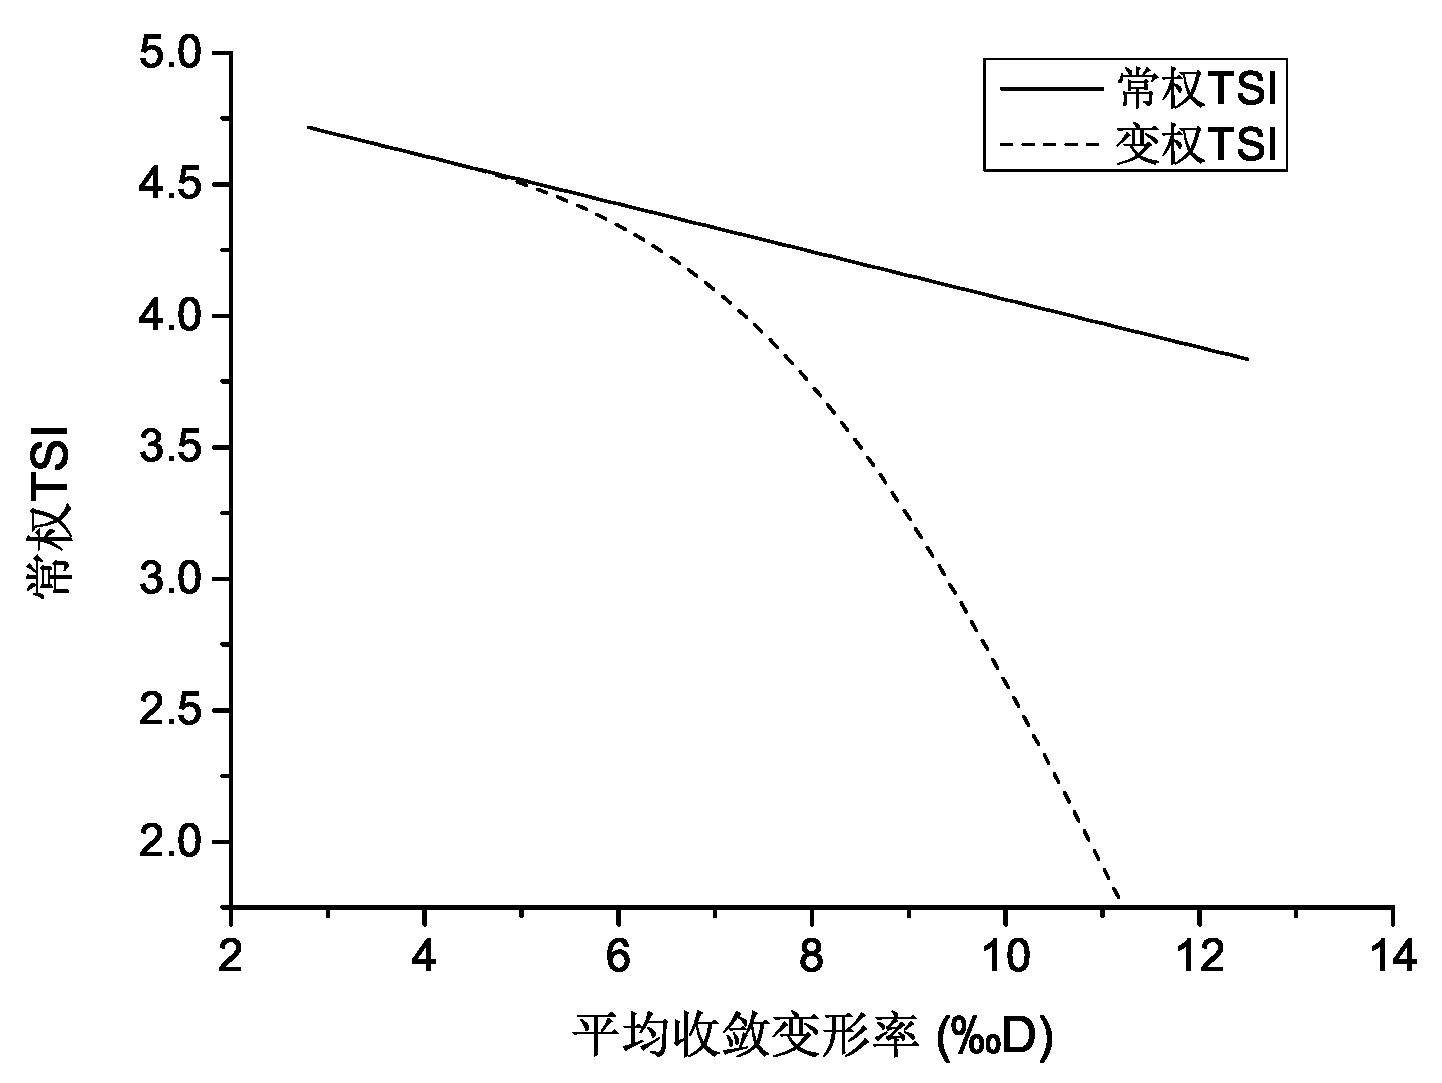
\includegraphics[width=0.7\textwidth]{chap2/const-change.eps}
    \caption{常权TSI与变权TSI曲线比较}
    \label{fig:常权TSI与变权TSI曲线比较}
\end{figure}

\subsection{空间网格TSI应用}

选取上海地铁1号线、2号线和4号线,并计算目前有监测和检测数据的区间的TSI值,如图~\ref{fig:上海地铁TSI指标计算结果}~所示,1号线沿线的TSI范围在1.4-3.5之间,其中人民广场-大世界和上海图书馆-徐家汇区间最为严重,评估结果比“一般”与“差”之间;2号线沿线的TSI范围在1.6-2.8之间,大部分处理“好”等级;4号线沿线的TSI范围在1.6-2.6之间,情况与2号线类似。另外,从图~\ref{fig:上海地铁TSI指标计算结果}~的地铁线路交汇处,如1号线与2号线的人民广场站附近,TSI计算结果在2.8左右,1号线与4号线的上海体育馆附近,TSI计算结果在2.0左右,且服役性能指标受很多外部因素的影响,如地质条件、上部荷载等,这些影响因素本身是存在空间关联性的。故本文假设地铁的服役性能指标值存在空间上的关联性,采用空间变异理论对其进行研究。

\begin{figure}[htb!]
    \centering
    \includegraphics[width=1.0\textwidth]{chap2/tsi-map.pdf}
    \caption{上海地铁TSI指标计算结果}
    \label{fig:上海地铁TSI指标计算结果}
\end{figure}

\begin{figure}[htb!]
    \centering
    \includegraphics[width=1.0\textwidth]{chap2/tsi-preprocess.pdf}
    \caption{上海地铁TSI正态性和趋势验证}
    \label{fig:上海地铁TSI正态性和趋势验证}
\end{figure}

应用空间变异理论要求研究变量是平稳的,可分析TSI计算结果是否近似正态分布,以及TSI结果在空间上是否存在某种趋势,结果如图~\ref{fig:上海地铁TSI正态性和趋势验证}~所示,通过QQPlot图和直方图可知,除了TSI在1.6左右的数据较多,TSI结果的分布基本符合正态分布,趋势分析中由南北方向和东西方向的散点图可知拟合直线接近水平,不存在明显趋势。绘制TSI变异函数图如图~\ref{fig:上海地铁TSI变异函数图}~,从图中可知变程在2500$m$,即TSI在空间上的关联性最长距离为2500$m$。

\begin{figure}[htb!]
    \centering
    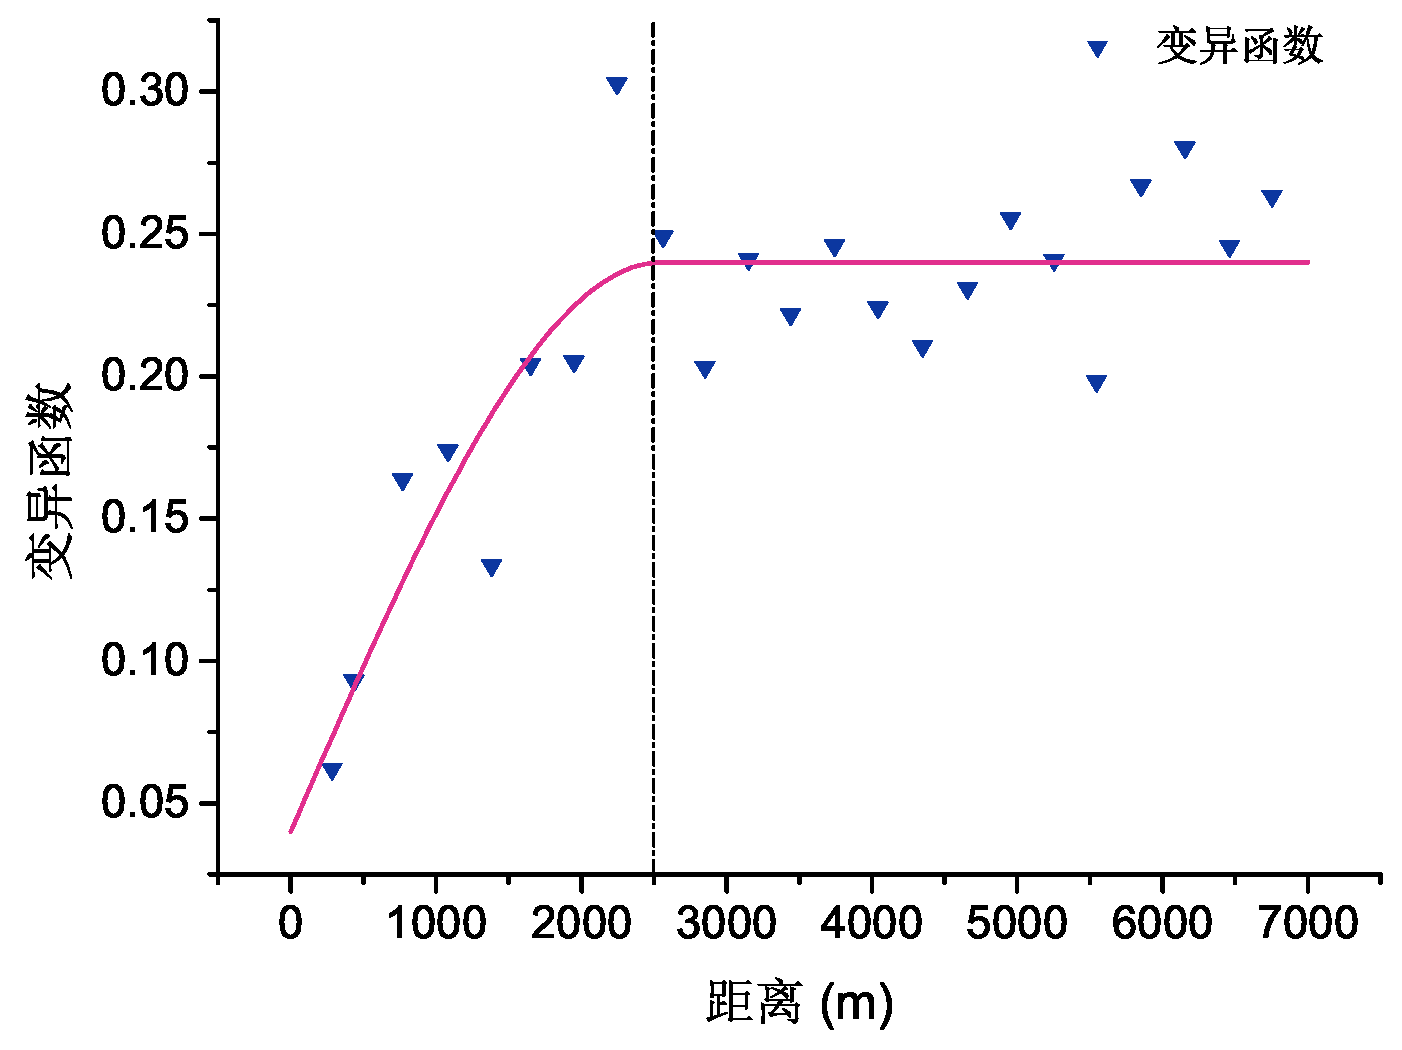
\includegraphics[width=0.7\textwidth]{chap2/semivariance.eps}
    \caption{上海地铁TSI变异函数图}
    \label{fig:上海地铁TSI变异函数图}
\end{figure}

\begin{figure}[htb!]
    \centering
    \includegraphics[width=1.0\textwidth]{chap2/tsi-interpolation.pdf}
    \caption{上海地铁TSI网格分析结果}
    \label{fig:上海地铁TSI网格分析结果}
\end{figure}

选取最长影响距离为2500$m$,克里金估计方法结果如图~\ref{fig:上海地铁TSI网格分析结果}~,图中可知两个TSI指标较高的区域,分别是人民广场站附近和徐家汇站附近,导致隧道服役性能劣化的因素很多,如隧道所处地质条件、上部荷载、周围扰动、地下水等因素,采用网格化TSI分析可宏观上对隧道空间服役性能进行评估。

%%%%%%%%%%%%%%%%%%%%%%%%%%%%%%%%%%%%%%%%%%%%%%%%%%%%%%%%%%%%%%%%%%%
\section{本章小结}

本章提出了考虑评估指标相关性和指标劣化程度的变权服役性能评估方法,该评估方法具备物理意义明确、简单高效的特点,具体内容包括:

(1)给出了盾构隧道服役性能相关的基本概念定义,和本章评估方法的基本假设;

(2)根据现有监测和病害数据,结合数据之间的相关性,选取六个评估指标,分别为相对沉降平均值${sett}_{a}$、平均差异沉降$set{{t}_{d\_a}}$、平均收敛变形率${cov}_{a}$、百环渗漏水面积${d}_{l}$、百环衬砌剥落面积${d}_{s}$、百环裂缝长度${d}_{c}$。

(3)基于专家打分法和偏最小二乘法,回归拟合得出TSI计算公式如下,并归纳总结了上海地铁隧道TSI结果分布和评估指标分布。
\begin{align}
  & TSI=0.77+0.16\sqrt{set{{t}_{a}}}+0.01set{{t}_{d\_a}}+0.09{{\operatorname{cov}}_{a}} \nonumber \\ 
 & \quad \quad \quad +0.08{{d}_{l}}+0.05{{d}_{c}}+0.50{{d}_{s}} \nonumber 
\end{align}

(4)采用分段变权函数对TSI指标在隧道全寿命周期的应用进行修正。

(5)采用空间变异理论将TSI指标在宏观上对地铁盾构隧道网络进行网格化评估。

TSI计算方法已被国家行业标准《城市轨道交通隧道结构养护技术规范》所采纳。


%!TEX root = ../thesis.tex
\chapter{盾构隧道服役性能预测}
\label{chap:prediction}

第~\ref{chap:tsi}~章主要介绍了如何采用当前的观测变量,对盾构隧道服役性能进行评估,由第~\ref{chap:tsi}~章的基本假设可知,TSI计算仅考虑当前时间点的数据,有时候根据已有数据对未来数据的预测同样很重要。对于盾构隧道监测和病害数据,有两个重要的维度:时间和空间。时间维度是指单一点的数据随着时间的发展而变化,空间维度是指不同监测点数据并不是独立的,例如临近的沉降点监测数据应该是相似,不同监测点数据之间存在空间关联性。本章主要内容是在历史监测数据基础上,建立时空数据的预测模型,为隧道服役性能预测提供支持。

本章采用时间序列(Time Series)方法对隧道数据进行预测,时间序列可以用于研究事物随时间的发展规律,是一种定量分析方法。时间序列认为数据与时间之间存在关联性,数据之间也具有前后相承的联系,同时数据因为各种外部原因还表现出随机性。时间序列的主要思想是采用历史数据和外部影响因素近似描述不同类型的时序数据,并建立稳定的模型从而预测数据的未来发展趋势。一组有序的数列:${{Y}_{1}},{{Y}_{2}},{{Y}_{3}}\cdots {{Y}_{t}}$(其中$t$代表时间序号),时间间隔均匀的,且是随机过程的一个实现,则该序列为时间序列。在本章开始之前,先介绍序列的一些基本概念。

(1)指标集$T$

指的是时间$t$的取值范围,对于随机过程,$t$是连续变化的,对于时间序列,$t$则是离散的,取$t$为$\left\{ 0,\pm 1,\pm 2,\pm 3\cdots  \right\}$,在实际中,$t$一般取$\left\{ 0,1,2,3\cdots  \right\}$。

(2)采样间隔$\Delta t$

即时间序列相邻数据之间的时间差,一般地时间序列分析要求数据采样间隔是一致的。

(3)平稳时间序列

大部分时间序列分析要求数据为平稳时间序列。定义为如果对于$\forall {{t}_{1}},{{t}_{2}},{{t}_{3}}\cdots {{t}_{n}}$,$h\in T$和任意的$n$,都有$\left( {{Y}_{{{t}_{1}}}},{{Y}_{{{t}_{2}}}}\cdots {{Y}_{{{t}_{n}}}} \right)$与$\left( {{Y}_{{{t}_{1}}+h}},{{Y}_{{{t}_{2}}+h}}\cdots {{Y}_{{{t}_{n}}+h}} \right)$同分布,则称该时间序列为平稳时间序列。

(4)白噪声序列

白噪声序列是特殊的平稳序列。定义为互相独立的序列变量$\left\{ {{Y}_{t}} \right\}$,对于任意$s\ne t$,如果$Cov({{Y}_{s}},{{Y}_{t}})=0$,则称该序列为白噪声序列。也即是说,白噪声序列在不同的时间点上的数据的协方差为0,无法采用历史数据来预测未来的数据,未来数据是无规律的。

\begin{figure}[htb!] 
    \centering 
    \begin{tabular}{c} 
        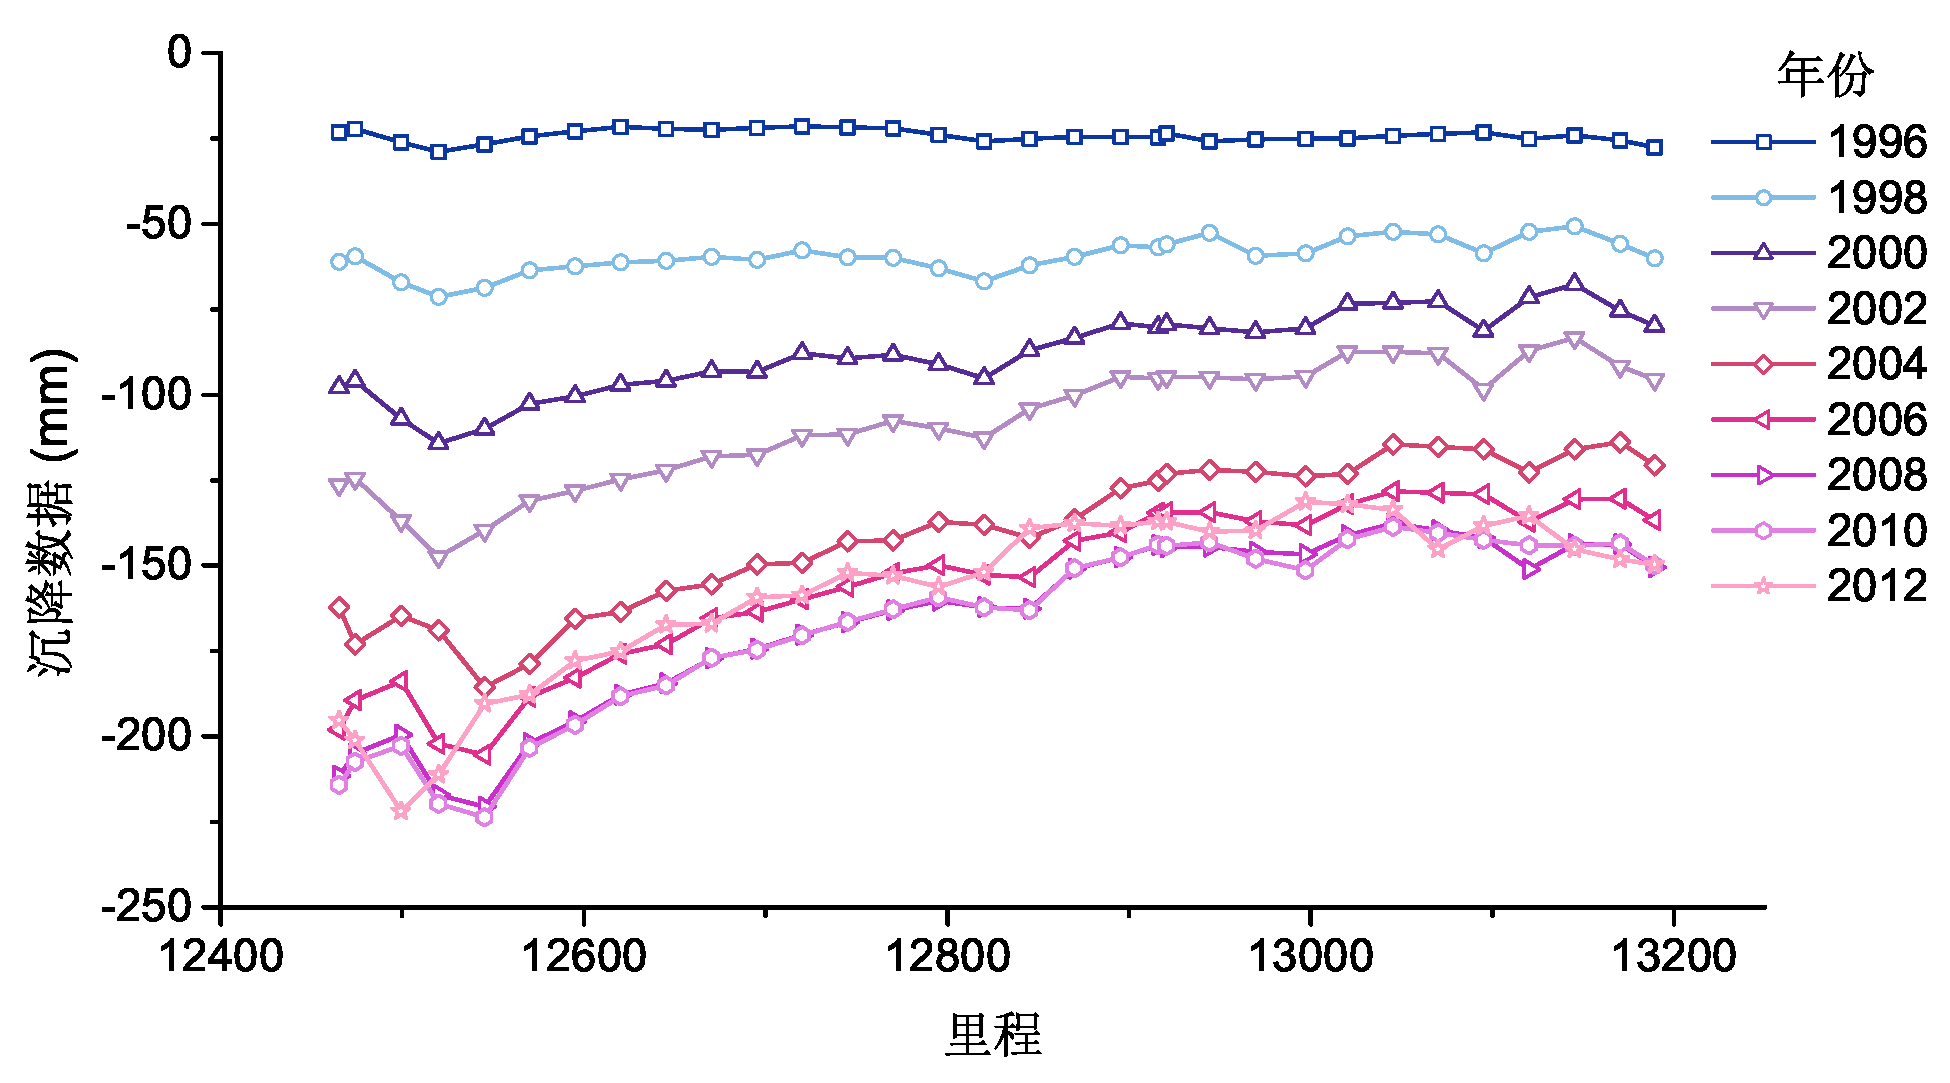
\includegraphics[width=1.0\textwidth]{chap3/sett-history.eps} \\ 
        (a)~区间不同年份沉降 \\
        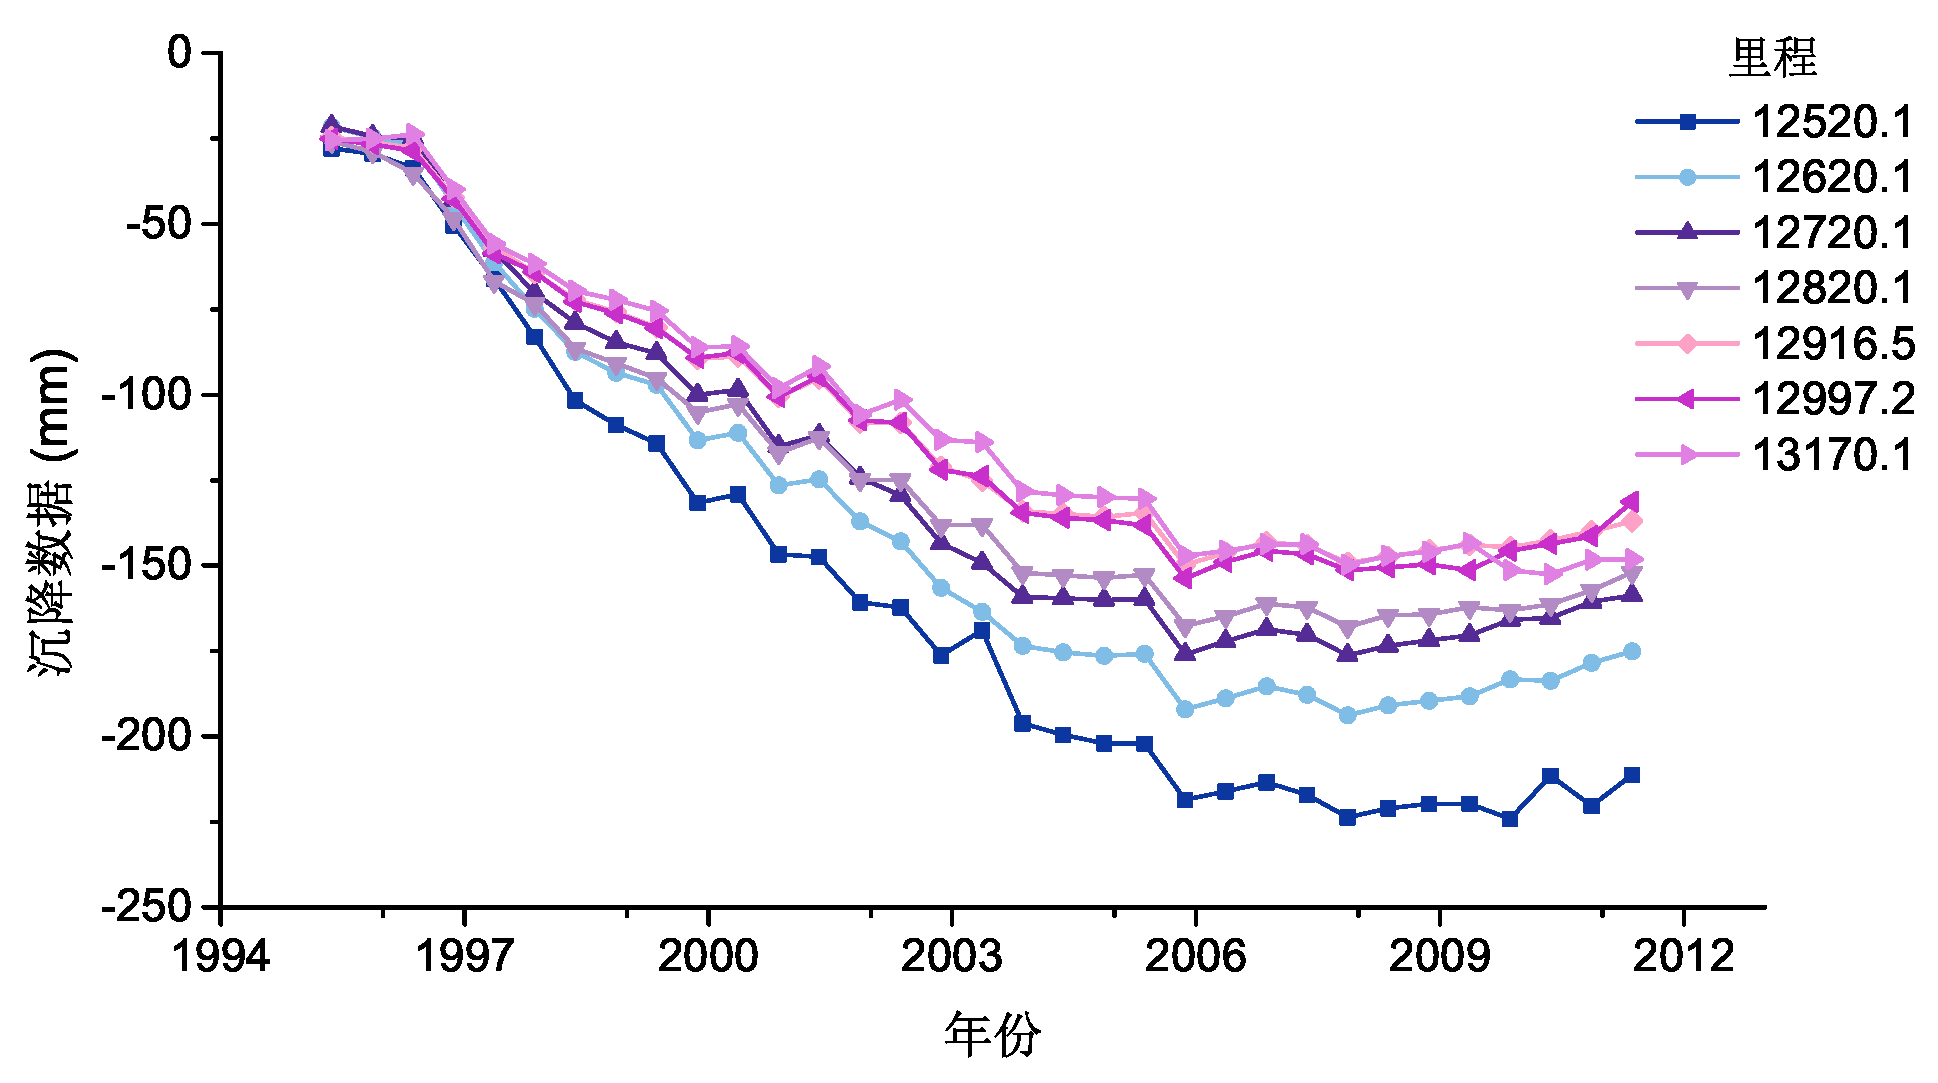
\includegraphics[width=1.0\textwidth]{chap3/sett-history2.eps} \\ 
        (b)~区间不同里程沉降 \\
    \end{tabular}
    \caption{地铁1号线新闸路-汉中路区间历史沉降} 
    \label{fig:地铁1号线新闸路-汉中路区间历史沉降} 
\end{figure}

%%%%%%%%%%%%%%%%%%%%%%%%%%%%%%%%%%%%%%%%%%%%%%%%%%%%%%%%%%%%%%%%%%%
\section{数据准备与处理}

%+++++++++++++++++++++++++++++++++++++++++++++++++++++++++++++++++%
\subsection{数据准备}

第~\ref{chap:tsi}~章采用沉降、收敛、渗漏水、裂缝和剥落评估隧道服役性能,对服役性能的预测即研究各个指标的退化模型。性能退化需建立在历年连续监测数据基础上,目前上海地铁对上述指标数据的采集情况如下:沉降数据从隧道建成开始,每年固定采集两次,如地铁1号线、2号线和4号线分别从1995年、1999年和2005年至今均有采集沉降数据;收敛数据在一开始并不作为日常监测的项目,随着近年对隧道横向变形的关注,这一指标才纳入监测范围,截止到2015年为止,地铁全线只在2011年、2012年和2014年进行过收敛数据的采集;对于病害数据,由于运营隧道里程长,人工检查速度慢,病害数据也只有在2011年和2012年进行过全线的检查,但随着病害采集车、无线传感、图像识别等技术的成熟,采集数据将会越来越多。

鉴于上述情况,本文只采用沉降数据作为研究对象,介绍预测方法原理及其应用,方法对于其他指标同样适用。以地铁1号线新闸路至汉中路区间为例,其历史沉降数据如图~\ref{fig:地铁1号线新闸路-汉中路区间历史沉降}~所示,整体来说,隧道的沉降曲线为两边高,中间低的形状(图~\ref{fig:地铁1号线新闸路-汉中路区间历史沉降}a),并且在隧道建成初期沉降速率快,随着运营年份的增加,沉降趋于稳定(图~\ref{fig:地铁1号线新闸路-汉中路区间历史沉降}b)。


%+++++++++++++++++++++++++++++++++++++++++++++++++++++++++++++++++%
\subsection{异常数据与缺失数据}

由于监测设备失灵、故障或人为失误、遗漏等原因,造成采集数据异常或者缺失,在作数据分析之前应对异常数据和缺失数据进行处理。异常数据一般可采用箱形图(Box-WhiskerPlot)进行处理,箱形图主要包含六个数据节点,分别为上边缘、上四分位数Q3、中位数、下四分位数Q1、下边缘和异常值,定义四分位距IQR=Q3-Q1,将Q3+1.5IQR和Q1-1.5IQR位置定义为异常值截断点,称其为内限,处于内限以外位置的点表示的数据可归为异常值。图~\ref{fig:地铁1号线新闸路-汉中路区间部分沉降箱形图}~所示为地铁1号线新闸路-汉中路区间部分沉降数据箱形图,从图中可知1996年4月和1998年4月采集的数据存在异常值,可将该数据删除后采用缺失数据处理方法补全。

\begin{figure}[htb!]
    \centering
    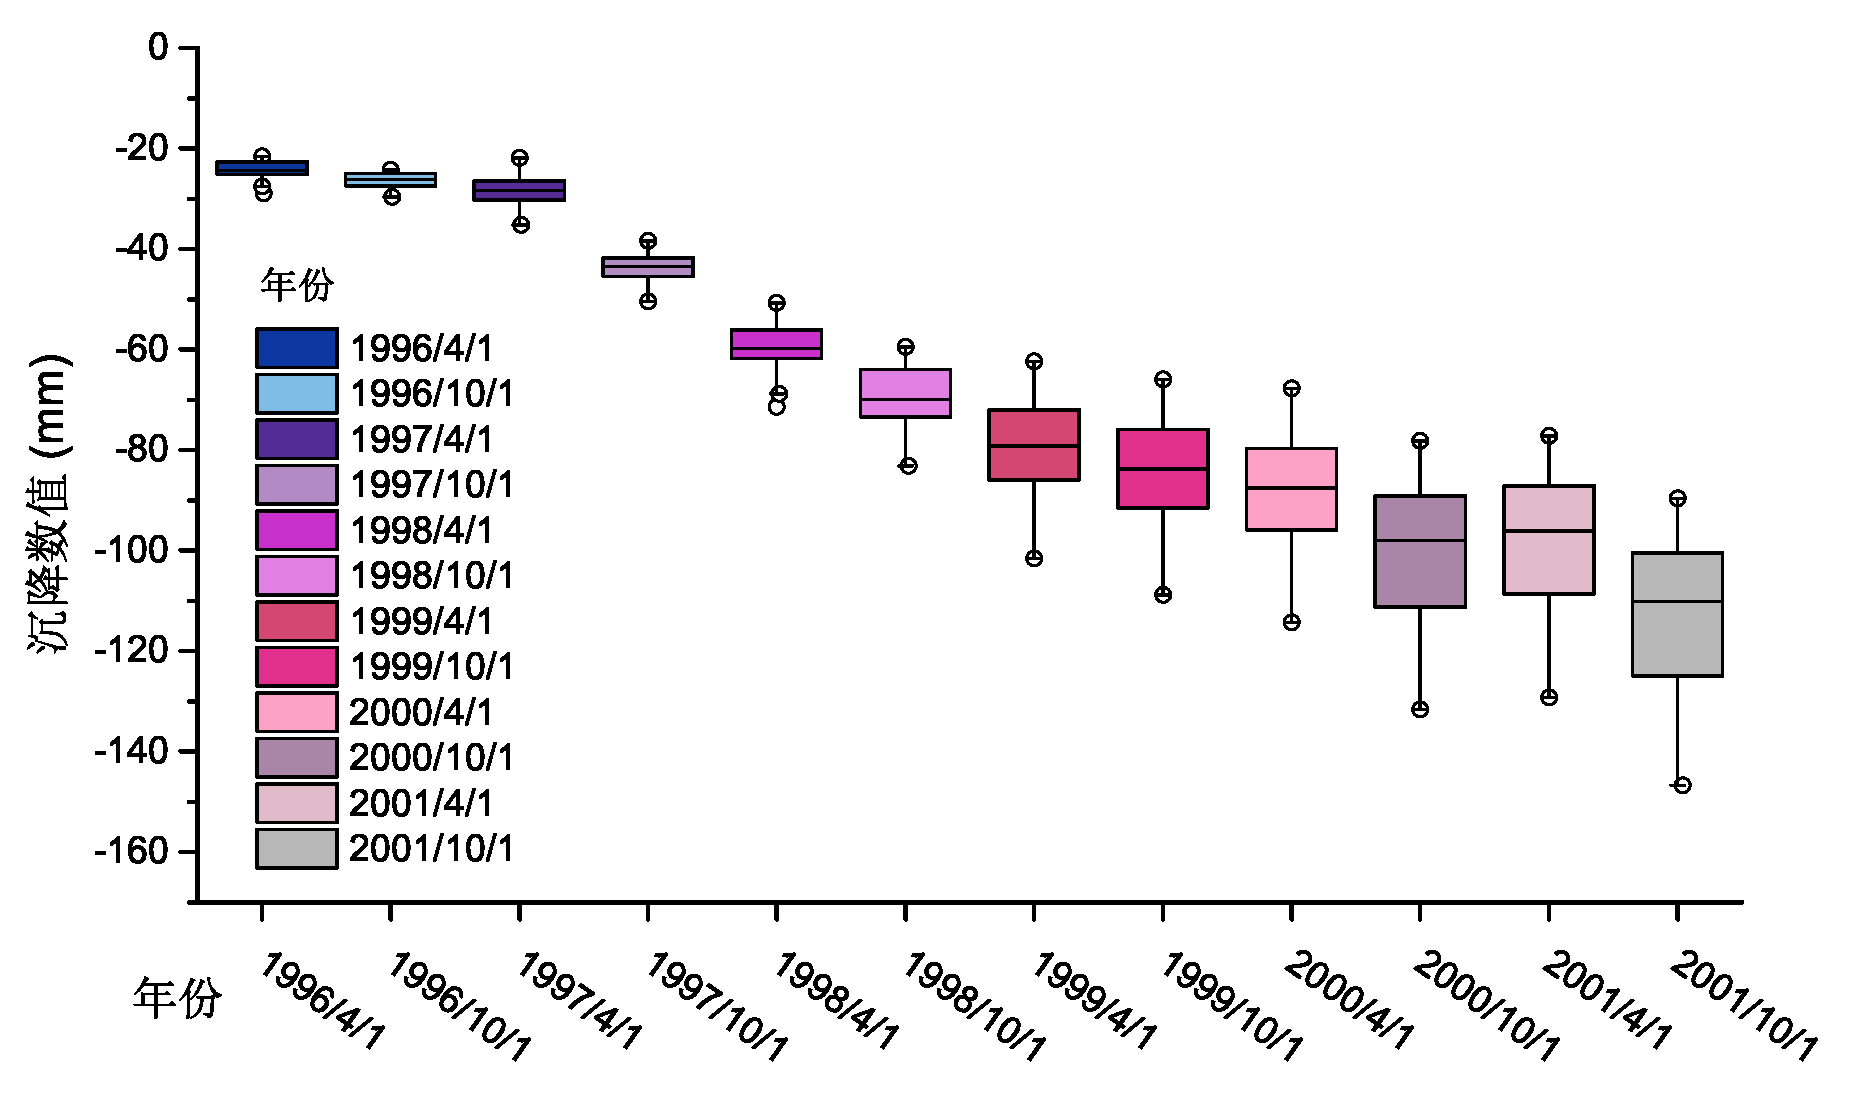
\includegraphics[width=1.0\textwidth]{chap3/boxplot.eps}
    \caption{地铁1号线新闸路-汉中路区间部分沉降箱形图}
    \label{fig:地铁1号线新闸路-汉中路区间部分沉降箱形图}
\end{figure}

常见的缺失数据处理方法有个案剔除法、均值替换法、回归替换法等,对于沉降数据的拟合可采用多项式、指数曲线、多段曲线、样条曲线等拟合,叶耀东(\citeyear{叶耀东2007软土地区运营地铁盾构隧道结构变形及健康诊断方法研究})提出三次均匀B样条曲线拟合实际隧道沉降,拟合方程为
\begin{equation}
    P(u)=\sum\limits_{i=0}^{n}{{{P}_{i}}{{N}_{i,k}}(u)}
\end{equation}
式中:${{P}_{i}}(i=0,1,\cdots ,n)$为沉降点,又称为德布尔点;${{N}_{i,k}}(u)(i=0,1,\cdots ,n)$称为$k$次规范B样条基函数。

本文采用三次样条曲线拟合的结果插值缺失数据较少的情况,在缺失数据较多时,上述方法的误差较大,则采用临近数据均值的方法插值,即取相邻里程的两个监测点,以及过去和未来一次的监测数据求和平均替代缺失数据。


%%%%%%%%%%%%%%%%%%%%%%%%%%%%%%%%%%%%%%%%%%%%%%%%%%%%%%%%%%%%%%%%%%%
\section{自回归与滑动平均时间序列模型}

%+++++++++++++++++++++++++++++++++++++++++++++++++++++++++++++++++%
\subsection{基本原理}

最出名的时间序列模型是由Box和Jenkins(\citeyear{box2015time})于1976年提出的自回归滑动平均时间序列(Autoregressive-Moving Average,ARMA),本节先简单介绍该模型的基本原理(EViews,\citeyear{noble2011eviews};潘红宇,\citeyear{cryer2011时间序列分析及应用})。

\subsubsection{自回归AR模型}

自回归模型就是用自身做回归变量,对于$p$阶自回归序列$\left\{ {{Y}_{t}} \right\}$满足方程:
\begin{align}
  \label{equ:AR1}
  & {{Y}_{t}}={{\rho }_{1}}{{Y}_{t-1}}+{{\rho }_{2}}{{Y}_{t-2}}+\cdots +{{\rho }_{p}}{{Y}_{t-p}}+{{\varepsilon }_{t}} \\ 
 & \quad =\sum\limits_{j=1}^{p}{{{\rho }_{j}}{{Y}_{t-j}}}+{{\varepsilon }_{t}} \nonumber
\end{align}
式中:${\varepsilon }_{t}$为新息项,包括了序列在$t$其无法用历史数据来解释的新新息,且${\varepsilon }_{t}$独立于${{Y}_{t-1}},{{Y}_{t-2}},{{Y}_{t-3}}\cdots $;${\rho }_{j}$为当前数据与历史数据的依赖关系系数。该式假设大于$p$阶滞后数据与当前数据没有关系。

为方便后续讨论,定义滞后算子$L$为
\begin{equation}
	\label{equ:lagL}
	{{L}^{k}}{{Y}_{t}}={{Y}_{t-k}}
\end{equation}
则式~\ref{equ:AR1}~可重写为
\begin{align}
  & {{Y}_{t}}=\sum\limits_{j=1}^{p}{{{\rho }_{j}}{{L}^{j}}{{Y}_{t}}}+{{\varepsilon }_{t}} \\ 
  \label{equ:lagL2}
 & \quad \rho (L){{Y}_{t}}={{\varepsilon }_{t}}
\end{align}
其中
\begin{equation}
	\label{equ:AR3}
	\rho (L)=1-\sum\limits_{j=1}^{p}{{{\rho }_{j}}{{L}^{j}}}
\end{equation}
为滞后算子多项式,如果该时间序列均值不为0,则设$t$时刻时间序列均值为${{\mu }_{t}}$,则式~\ref{equ:lagL2}~可以写成
\begin{equation}
	\rho (L)({{Y}_{t}}-{{\mu }_{t}})={{\varepsilon }_{t}}
\end{equation}
对于$p$阶AR模型,假设均值${{\mu }_{t}}$为外部变量${X'}_{t}$的线性组合,即${{\mu }_{t}}={{{X}'}_{t}}\beta $,则$p$阶的AR(p)模型最终如下:
\begin{gather}
  	{{Y}_{t}}={{{{X}'}}_{t}}\beta +{{u}_{t}} \\ 
 	{{u}_{t}}={{\rho }_{1}}{{u}_{t-1}}+{{\rho }_{2}}{{u}_{t-2}}+\cdots +{{\rho }_{p}}{{u}_{t-p}}+{{\varepsilon }_{t}} \\ 
 	{{Y}_{t}}={{{{X}'}}_{t}}\beta +\sum\limits_{j=1}^{p}{{{\rho }_{j}}({{Y}_{t-j}}-{{{{X}'}}_{t-j}}\beta )+}{{\varepsilon }_{t}} \\ 
 	\left( 1-\sum\limits_{j=1}^{p}{{{\rho }_{j}}{{L}^{j}}} \right)({{Y}_{t}}-{{{{X}'}}_{t}}\beta )={{\varepsilon }_{t}} 
\end{gather}

\subsubsection{滑动平均MA模型}

滑动平均MA模型的$q$阶形式为
\begin{align}
  & {{Y}_{t}}={{\varepsilon }_{t}}+{{\theta }_{1}}{{\varepsilon }_{t-1}}+{{\theta }_{2}}{{\varepsilon }_{t-2}}+\cdots +{{\theta }_{q}}{{\varepsilon }_{t-q}} \nonumber \\ 
 & \quad ={{\varepsilon }_{t}}+\sum\limits_{j=1}^{q}{{{\theta }_{j}}{{\varepsilon }_{t-j}}} \\ 
 & \quad =\theta (L){{\varepsilon }_{t}} \nonumber
\end{align}
式中:${\theta }_{j}$为新息项的系数,且
\begin{equation}
	\theta (L)=1+\sum\limits_{j=1}^{q}{{{\theta }_{j}}{{L}^{j}}}
\end{equation}
是滑动平均模型的${\theta }$多项式,代表MA模型的特性,若MA模型的均值不为0,则可记
\begin{equation}
	\label{equ:MA1}
	{{Y}_{t}}-\mu =\theta (L){{\varepsilon }_{t}}
\end{equation}

\subsubsection{自回归滑动平均ARMA模型}

自回归滑动平均模型是由AR模型和MA模型组合得到,结合式~\ref{equ:AR3}~和式~\ref{equ:MA1}~可得
\begin{equation}
	\rho (L)({{Y}_{t}}-{{\mu }_{t}})=\theta (L){{\varepsilon }_{t}}
\end{equation}
对于$p$阶AR模型和$q$阶MA模型的组合命名为ARMA(p,q)。最简单的ARMA模型由1阶AR和1阶MA组成的ARMA(1,1),如下:
\begin{gather}
 	{{Y}_{t}}={{{{X}'}}_{t}}\beta +{{u}_{t}} \\ 
	{{u}_{t}}=\rho {{u}_{t-1}}+{{\varepsilon }_{t}}+\theta {{\varepsilon }_{t-1}}
\end{gather}
式中:$\rho$为一阶AR模型参数;$\theta$为一阶MA模型参数。代入后ARMA(1,1)模型可写为
\begin{align}
  & {{Y}_{t}}={{{{X}'}}_{t}}\beta +\rho {{u}_{t-1}}+{{\varepsilon }_{t}}+\theta {{\varepsilon }_{t-1}} \\ 
 & ={{{{X}'}}_{t}}\beta +\rho ({{Y}_{t-1}}-{{{{X}'}}_{t-1}}\beta )+{{\varepsilon }_{t}}+\theta {{\varepsilon }_{t-1}}
\end{align}
采用滞后算子$L$可简写为
\begin{equation}
	(1-\rho L)({{Y}_{t}}-{{{X}'}_{t}}\beta )=(1+\theta L){{\varepsilon }_{t}}
\end{equation}

%+++++++++++++++++++++++++++++++++++++++++++++++++++++++++++++++++%
\subsection{模型建立}
\label{chap:armamodelbuilding}

上述介绍的AR、MA和ARMA模型不存在哪个模型是最优的,它们分别描述了时间序列的自然属性,在建立时间序列模型时需选择合适的模型和滞后阶数。时间序列模型要求分析的序列是平稳的,但在实际中大部分的序列都是非平稳的,需将非平稳时间序列转化成平稳时间序列。一般的序列通过一阶差分(式~\ref{equ:diff1}~)或二阶差分(式~\ref{equ:diff2}~)可转换成平稳序列(Hamilton,\citeyear{hamilton1994time})。
\begin{gather}
	\label{equ:diff1}
	\nabla {{Y}_{t}}={{Y}_{t}}-{{Y}_{t-1}} \\ 
	\label{equ:diff2}
	{{\nabla }^{2}}{{Y}_{t}}=\nabla \nabla {{Y}_{t}}=({{Y}_{t}}-{{Y}_{t-1}})-({{Y}_{t-1}}-{{Y}_{t-2}}) 
\end{gather}
定量化的判断序列是否平稳可采用Dickey-Fuller单位根进行验证检验(Dickey和Fuller,\citeyear{dickey1979distribution})。

对于观测到的时间序列${{Y}_{1}},{{Y}_{2}},\cdots ,{{Y}_{n}}$,定义时间序列的自相关函数(Autocorrelation Function,ACF)为
\begin{equation}
	{{r}_{k}}=\frac{\sum\limits_{t=k+1}^{n}{({{Y}_{t}}-\bar{Y})({{Y}_{t-k}}-\bar{Y})}}{\sum\limits_{t=1}^{n}{{{({{Y}_{t}}-\bar{Y})}^{2}}}},k=1,2\cdots 
\end{equation}
定义消除中间介入变量${{Y}_{t-1}},{{Y}_{t-2}},{{Y}_{t-3}},\cdots ,{{Y}_{t-k+1}}$的影响后$Y_t$和$Y_{t-k}$的相关系数函数为偏相关系数(Partial Autocorrelation Function,PACF),即
\begin{equation}
	{{\rho }_{kk}}=Corr({{Y}_{t}},{{Y}_{t-k}}|{{Y}_{t-1}},{{Y}_{t-2}},\cdots ,{{Y}_{t-k+1}})
\end{equation}

通过观察自相关图与偏相关图可确定ARMA(p,q)模型的具体形式,有两个相关概念:(1)拖尾:指的是ACF或者PACF随滞后阶数呈几何衰减;(2)截尾:指的是ACF或者PACF在某一阶不为0,之后突然接近或者等于0。

AR(p)模型,从自相关函数ACF来看,在自回归方程的基础上可以很简单构造ACF,自相关系数等于${{\rho }^{k}}$(${\rho }$为自回归系数,$k$为滞后数),对于平稳时间序列,$\left| \rho  \right|<1$,所以当${\rho }>0$时,ACF呈现为指数式衰减至0.当${\rho }<0$时,ACF则正负交替呈指数衰减至0,整体表现则是正弦式衰减;从偏相关函数PACF来看,其与自回归方程的形式完全一样,只是自回归方程只有滞后$p$期,而PACF则有更多的滞后项。于是乎,当$k\le p$,偏相关系数不等于0,当$k>p$,偏相关系数等于0,明显呈现出截尾现象。

MA(q)模型,从自相关函数ACF来看,在移动平均方程的基础上也可以很简单地构造自相关系数,这时候的自相关函数为分段函数,当$k\le q$,偏相关系数不等于0,当$k>q$,偏相关系数等于0,明显呈现出截尾现象;从偏相关函数PACF来看,任何一个可逆的MA(q)过程都可以转换成一个无限阶、系数按几何衰减的AR过程(将白噪声替换为序列的滞后形式即可),呈现拖尾现象。与AR(p)不同的是,当$\theta >0$($\theta$为移动平均系数)时,PACF呈现为交替式正弦衰减。当$\theta <0$时,PACF则呈指数衰减至0。ARMA(p,q)模型则是两者的结合,总结如表~\ref{tab:armaarma}~所示。

\begin{table}[htb!]
  \centering
  \caption{AR、MA、ARMA模型识别}
    \begin{tabular}{?m{11em}<{\centering}"m{9em}<{\centering}"m{9em}<{\centering}?}
    \thickhline
    模型定阶  & 自相关系数 & 偏相关系数 \bigstrut\\
    \thinhline
    AR(p)模型 & 拖尾    & p阶截尾 \bigstrut\\
    \thinhline
    MA(q)模型 & q阶截尾  & 拖尾 \bigstrut\\
    \thinhline
    ARMA(p,q)模型 & 拖尾    & 拖尾 \bigstrut\\
    \thickhline
    \end{tabular}%
  \label{tab:armaarma}%
\end{table}%

除了根据拖尾和截尾的属性,还可以采用AIC(Akaike Information Criterion)(Akaike,\citeyear{akaike2011akaike})和BIC(Schwarz Criterion)(Schwarz,\citeyear{schwarz1978estimating})准则进行模型识别。在确定了模型阶数后,可采用矩估计、最小二乘估计和极大似然估计等方法进行参数估计。

%+++++++++++++++++++++++++++++++++++++++++++++++++++++++++++++++++%
\subsection{模型验证}

时间序列模型的验证可验证模型残差$\left\{ {{\varepsilon }_{t}} \right\}$是否为白噪声,若残差不是白噪声,则说明残差中的信息并未完全提取,应考虑重新选定模型。

白噪声验证可通过${{\chi }^{2}}$检验验证。${{\chi }^{2}}$是一种简单又高效的检验方法,其证明$m$个独立的$N(0,1)$分布的随机变量的平方和为自由度为$m$的${{\chi }^{2}}$分布,残差的自相关函数为
\begin{equation}
	{{\gamma }_{k}}(\varepsilon )=\frac{\sum\limits_{t=1}^{N-k}{{{\varepsilon }_{t}}{{\varepsilon }_{t+k}}}}{\sum{\varepsilon _{t}^{2}}}
\end{equation}
当$n\to \infty$,$\sqrt{N}{{\gamma }_{k}}(\varepsilon )\tilde{\ }N(0,1)(k=1,2,\cdots ,m)$。

原假设:残差序列之间相互独立。则残差${{\chi }^{2}}$统计量
\begin{equation}
	{{Q}_{m}}=\sum\limits_{k=1}^{m}{{{\left[ \sqrt{N}{{\gamma }_{k}}(\varepsilon ) \right]}^{2}}=n\sum\limits_{k=1}^{m}{\gamma _{k}^{2}(\varepsilon )}}
\end{equation}
式中:$n$为观测数据个数;$m$为最大的时滞。

在显著性水平$\alpha $下,记${{\chi }^{2}}$为$\chi _{\alpha }^{2}$。比较${{\chi }^{2}}$与$Q_m$的大小,如果${{Q}_{m}}\le \chi _{\alpha }^{2}$,则接受原假设,即残差为白噪声;反之,拒绝原假设,即残差不是白噪声。


%+++++++++++++++++++++++++++++++++++++++++++++++++++++++++++++++++%
\subsection{盾构隧道ARMA模型建模}

根据上述时间序列理论,建立时间序列模型大致可以分为稳定性判断、模型识别和模型验证几个步骤,如图~\ref{fig:ARMA时间序列模型建模流程图}~所示。

\begin{figure}[htb!]
    \centering
    \includegraphics[width=0.55\textwidth]{chap3/time-series-process.pdf}
    \caption{ARMA时间序列模型建模流程图}
    \label{fig:ARMA时间序列模型建模流程图}
\end{figure}

\subsubsection{稳定性判断}

以上海地铁1号新闸路至汉中路下行线,里程为12916.05的沉降监测点为例,介绍沉降ARMA模型建立。首先根据原始数据计算自相关和偏相关图,如表~\ref{tab:原始沉降数据的自相关与偏相关系数}~所示。由自相关图可看到,自相关系数递减缓慢,并且在时滞为10时候,仍大于两倍标准差范围,可以判断沉降数据存在趋势。另一方面,观察图~\ref{fig:地铁1号线新闸路-汉中路区间历史沉降}b~可以看出数据存在明显的趋势,在一开始数据增加速度较快,后期则逐渐减缓,且存在一定的波动。

可考虑采用线性回归或者差分的方法将数据转化为平稳数据。对于沉降数据,随着隧道运营时间增长,沉降逐渐趋于稳定,甚至沉降还会有回弹,很难用某一回归模型进行拟合,而且回归模型对于未来的数据趋势拟合也不一定很好。故本文采用差分的方法进行数据平稳化处理。根据~\ref{chap:armamodelbuilding}~小节采用单位根ADF检验判断序列是否存在单位根,若ADF的统计量比置信区间的临界值大,则不能拒绝序列存在单位根的假设,即序列是非平稳的。一般取置信区间为0.5\%。计算结果如表~\ref{tab:沉降数据差分稳定性分析}~所示,原始数据的单位根t统计量为-3.882999,显著性水平为0.0058,不足以拒绝原始数据存在单位根的假设。一阶差分的单位根t统计量为-2.268996,显著性水平为0.1880,一阶差分后的序列仍然不是平稳的。二阶差分的单位根t统计量为-7.312877,足以拒绝原假设,即沉降数据经过二阶差分后为平稳数据。但是有一点需要注意,虽然差分运算可以将数据平稳化,但差分后数据的物理意义可能存在难以解释的问题,如沉降数据的一阶差分为沉降速率,二阶差分则表示沉降加速度。

\begin{table}[htb!]
  \centering
  \caption{原始沉降数据的自相关与偏相关系数}
    \begin{tabular}{?c"m{8em}<{\centering}"m{8em}<{\centering}"c"c"c"c?}
    \thickhline
    阶数    & 自相关系数 & 偏相关系数 & AC    & PAC   & Q-Stat & Prob \bigstrut\\
    \thinhline
    1     & \multirow{12}[24]{*}{\includegraphics[width=8em,height=22.2em]{chap3/ACF1.pdf}} & \multirow{12}[24]{*}{\includegraphics[width=8em,height=22.2em]{chap3/PACF1.pdf}} & 0.910  & 0.910  & 29.893  & 0.000  \bigstrut\\
\cline{1-1}\cline{4-7}    2     &       &       & 0.813  & -0.086  & 54.550  & 0.000  \bigstrut\\
\cline{1-1}\cline{4-7}    3     &       &       & 0.702  & -0.142  & 73.500  & 0.000  \bigstrut\\
\cline{1-1}\cline{4-7}    4     &       &       & 0.606  & 0.038  & 88.134  & 0.000  \bigstrut\\
\cline{1-1}\cline{4-7}    5     &       &       & 0.519  & -0.010  & 99.237  & 0.000  \bigstrut\\
\cline{1-1}\cline{4-7}    6     &       &       & 0.436  & -0.052  & 107.360  & 0.000  \bigstrut\\
\cline{1-1}\cline{4-7}    7     &       &       & 0.353  & -0.056  & 112.910  & 0.000  \bigstrut\\
\cline{1-1}\cline{4-7}    8     &       &       & 0.271  & -0.056  & 116.300  & 0.000  \bigstrut\\
\cline{1-1}\cline{4-7}    9     &       &       & 0.188  & -0.069  & 118.000  & 0.000  \bigstrut\\
\cline{1-1}\cline{4-7}    10    &       &       & 0.116  & 0.006  & 118.680  & 0.000  \bigstrut\\
\cline{1-1}\cline{4-7}    11    &       &       & 0.032  & -0.151  & 118.730  & 0.000  \bigstrut\\
\cline{1-1}\cline{4-7}    12    &       &       & -0.039  & -0.007  & 118.820  & 0.000  \bigstrut\\
    \thickhline
    \end{tabular}%
  \label{tab:原始沉降数据的自相关与偏相关系数}%
\end{table}%

\begin{table}[htb!]
  \centering
  \caption{沉降数据差分稳定性分析}
    \begin{tabular}{?m{8em}<{\centering}"m{12em}<{\centering}"m{7em}<{\centering}"c?}
    \thickhline
    \multicolumn{2}{?c"}{原始数据} & t统计量  & 显著性水平 \bigstrut\\
    \thinhline
    \multicolumn{2}{?c"}{Dickey-Fuller单位根} & -3.882999  & 0.0058  \bigstrut\\
    \thinhline
    \multirow{3}[6]{*}{检验的临界值} & 1\%显著性水平 & -3.661661  &  \bigstrut\\
\cline{2-4}          & 5\%显著性水平 & -2.960411  &  \bigstrut\\
\cline{2-4}          & 10\%显著性水平 & -2.619160  &  \bigstrut\\
    \thinhline
    \multicolumn{2}{?c"}{一阶差分} &       &  \bigstrut\\
    \thinhline
    \multicolumn{2}{?c"}{Dickey-Fuller单位根} & -2.268996  & 0.1880  \bigstrut\\
    \thinhline
    \multirow{3}[6]{*}{检验的临界值} & 1\%显著性水平 & -3.670170  &  \bigstrut\\
\cline{2-4}          & 5\%显著性水平 & -2.963972  &  \bigstrut\\
\cline{2-4}          & 10\%显著性水平 & -2.621007  &  \bigstrut\\
    \thinhline
    \multicolumn{2}{?c"}{二阶差分} &       &  \bigstrut\\
    \thinhline
    \multicolumn{2}{?c"}{Dickey-Fuller单位根} & -7.312877  & 0.0000  \bigstrut\\
    \thinhline
    \multirow{3}[6]{*}{检验的临界值} & 1\%显著性水平 & -3.689194  &  \bigstrut\\
\cline{2-4}          & 5\%显著性水平 & -2.971853  &  \bigstrut\\
\cline{2-4}          & 10\%显著性水平 & -2.625121  &  \bigstrut\\
    \thickhline
    \end{tabular}%
  \label{tab:沉降数据差分稳定性分析}%
\end{table}%

\subsubsection{模型识别}

确定二阶差分形式为稳定序列后,绘制沉降二阶差分的自相关和偏相关函数,如表~\ref{tab:沉降数据二阶差分的自相关与偏相关系数}~所示。由表中可知,在时滞大于4的时候,自回归系数大小落入两倍标准差范围内,在时滞大于3的时候,偏回归系数大小落入两倍标准差范围内,ACF和PACF均有拖尾的现象,可尝试ARMA(3,4)阶数以下的ARMA模型,如AR(1)、AR(2)、AR(3)、MA(1)、MA(2)、MA(3)、MA(4)、AR(1,1)、AR(1,2)、AR(1,3)等,根据~\ref{chap:armamodelbuilding}~小节理论,采用极大似然法对模型参数进行估计,计算参数的t检验值,如表~\ref{tab:不同ARMA模型的参数估计}~所示,并计算了各个模型的残差平方和、AIC和BIC值,如表~\ref{tab:不同ARMA模型的残差平方和AIC和BIM}~所示。

\begin{table}[htb!]
  \centering
  \caption{沉降数据二阶差分的自相关与偏相关系数}
    \begin{tabular}{?c"m{8em}<{\centering}"m{8em}<{\centering}"c"c"c"c?}
    \thickhline
    阶数    & 自相关系数 & 偏相关系数 & AC    & PAC   & Q-Stat & Prob \bigstrut\\
    \thinhline
    1     & \multirow{12}[24]{*}{\includegraphics[width=8em,height=22.2em]{chap3/ACF2.pdf}} & \multirow{12}[24]{*}{\includegraphics[width=8em,height=22.2em]{chap3/PACF2.pdf}} & -0.705  & -0.705  & 16.929  & 0.000  \bigstrut\\
\cline{1-1}\cline{4-7}    2     &       &       & 0.436  & -0.120  & 23.634  & 0.000  \bigstrut\\
\cline{1-1}\cline{4-7}    3     &       &       & -0.464  & -0.413  & 31.510  & 0.000  \bigstrut\\
\cline{1-1}\cline{4-7}    4     &       &       & 0.429  & -0.138  & 38.483  & 0.000  \bigstrut\\
\cline{1-1}\cline{4-7}    5     &       &       & -0.305  & -0.057  & 42.137  & 0.000  \bigstrut\\
\cline{1-1}\cline{4-7}    6     &       &       & 0.246  & -0.037  & 44.621  & 0.000  \bigstrut\\
\cline{1-1}\cline{4-7}    7     &       &       & -0.285  & -0.157  & 48.077  & 0.000  \bigstrut\\
\cline{1-1}\cline{4-7}    8     &       &       & 0.327  & 0.084  & 52.824  & 0.000  \bigstrut\\
\cline{1-1}\cline{4-7}    9     &       &       & -0.351  & -0.162  & 58.563  & 0.000  \bigstrut\\
\cline{1-1}\cline{4-7}    10    &       &       & 0.307  & -0.117  & 63.148  & 0.000  \bigstrut\\
\cline{1-1}\cline{4-7}    11    &       &       & -0.237  & 0.008  & 66.020  & 0.000  \bigstrut\\
\cline{1-1}\cline{4-7}    12    &       &       & 0.214  & -0.062  & 68.491  & 0.000  \bigstrut\\
    \thickhline
    \end{tabular}%
  \label{tab:沉降数据二阶差分的自相关与偏相关系数}%
\end{table}%

根据模型的参数估计结果与各种统计量,选择模型参数时应综合考虑以下几个方面:(1)模型的参数估计值是否是显著的,在模拟结果差不多的情况下,参数估计是显著的可信度会更高,应优先选择;(2)信息量最小准则与模型精确准则,即需要兼顾模型的残差平方和大小、AIC值和BIC值,上述值越小,代表模型模拟的结果越好;(3)结合实际应用,应考虑模型的选择是否简单,以及有较好的物理意义。由表~\ref{tab:不同ARMA模型的残差平方和AIC和BIM}~可知残差平方和较小的模型有ARMA(3,0)、ARMA(0,4)、ARMA(3,1)ARMA(3,2)四个模型,模型所有的参数估计均显著的只有ARMA(3,0),其余模型有较多的参数估计不显著。综合考虑最后选择ARMA(3,0),即AR(3)模型作为沉降预测时间序列模型。

\begin{table}[htb!]
  \centering
  \caption{不同ARMA模型的参数估计}
    \begin{tabular}{?m{10em}<{\centering}"c"c"c"c"c"c"c?}
    \thickhline
    ARMA模型 & ar(1) & ar(2) & ar(3) & ma(1) & ma(2) & ma(3) & ma(4) \bigstrut\\
    \thinhline
    ARMA(1,0) & *-0.68 & -     & -     & -     & -     & -     & - \bigstrut\\
    \thinhline
    ARMA(2,0) & *-0.78 & -0.13  & -     & -     & -     & -     & - \bigstrut\\
    \thinhline
    ARMA(3,0) & *-0.89 & *-0.60 & *-0.51 & -     & -     & -     & - \bigstrut\\
    \thinhline
    ARMA(0,1) & -     & -     & -     & *-0.83 & -     & -     & - \bigstrut\\
    \thinhline
    ARMA(0,2) & -     & -     & -     & *-1.15 & 0.35  & -     & - \bigstrut\\
    \thinhline
    ARMA(0,3) & -     & -     & -     & *-1.16 & 0.33  & 0.04  & - \bigstrut\\
    \thinhline
    ARMA(0,4) & -     & -     & -     & *-1.01 & 0.18  & -0.38  & 0.47  \bigstrut\\
    \thinhline
    ARMA(1,1) & -0.36  & -     & -     & *-0.73 & -     & -     & - \bigstrut\\
    \thinhline
    ARMA(1,2) & *-0.91 & -     & -     & -0.04  & *-0.58 & -     & - \bigstrut\\
    \thinhline
    ARMA(2,1) & -0.29  & 0.10  & -     & *-0.76 & -     & -     & - \bigstrut\\
    \thinhline
    ARMA(2,2) & -0.94  & -0.03  & -     & -0.02  & -0.58  & -     & - \bigstrut\\
    \thinhline
    ARMA(3,1) & *-0.56 & -0.34  & -0.47  & -0.47  & -     & -     & - \bigstrut\\
    \thinhline
    ARMA(3,2) & -0.49 & -0.35 & *-0.49 & -0.55 & 0.08  & -     & - \bigstrut\\
    \thickhline
    \multicolumn{8}{l}{注:*号代表参数估计的t检验结果在显著性水平0.5\%下是显著的}
    \end{tabular}%
  \label{tab:不同ARMA模型的参数估计}%
\end{table}%

\begin{table}[htb!]
  \centering
  \caption{不同ARMA模型的残差平方和、AIC和BIM}
    \begin{tabular}{?m{10em}<{\centering}"m{8em}<{\centering}"m{7em}<{\centering}"m{7em}<{\centering}?}
    \thickhline
    ARMA模型 & 残差平方和 & AIC   & BIC \bigstrut\\
    \thinhline
    ARMA(1,0) & 1191.820  & 6.636450  & 6.728965  \bigstrut\\
    \thinhline
    ARMA(2,0) & 1172.360  & 6.685934  & 6.824707  \bigstrut\\
    \thinhline
    ARMA(3,0) & 891.432  & 6.504296  & 6.689326  \bigstrut\\
    \thinhline
    ARMA(0,1) & 1097.819  & 6.571083  & 6.663599  \bigstrut\\
    \thinhline
    ARMA(0,2) & 973.289  & 6.527866  & 6.666639  \bigstrut\\
    \thinhline
    ARMA(0,3) & 969.608  & 6.590446  & 6.775476  \bigstrut\\
    \thinhline
    ARMA(0,4) & 828.705  & 6.530977  & 6.762265  \bigstrut\\
    \thinhline
    ARMA(1,1) & 977.859  & 6.527053  & 6.665826  \bigstrut\\
    \thinhline
    ARMA(1,2) & 906.856  & 6.517413  & 6.702444  \bigstrut\\
    \thinhline
    ARMA(2,1) & 973.214  & 6.585157  & 6.770187  \bigstrut\\
    \thinhline
    ARMA(2,2) & 906.244  & 6.581513  & 6.812801  \bigstrut\\
    \thinhline
    ARMA(3,1) & 824.48 & 6.502938 & 6.734226 \bigstrut\\
    \thinhline
    ARMA(3,2) & 822.4791 & 6.566253 & 6.843799 \bigstrut\\
    \thickhline
    \end{tabular}%
  \label{tab:不同ARMA模型的残差平方和AIC和BIM}%
\end{table}%

\subsubsection{模型验证}

\begin{figure}[htb!] 
    \centering 
    \begin{tabular}{c} 
        \includegraphics[width=0.7\textwidth]{chap3/diff2data.eps} \\ 
        (a)~二阶差分原始数据与预测数据图 \\
        \includegraphics[width=0.7\textwidth]{chap3/ar3-residual.eps} \\ 
        (b)~二阶差分预测残差图 \\
    \end{tabular}
    \caption{AR(3)模型结果图} 
    \label{fig:AR3模型结果图} 
\end{figure}

绘制AR(3)模型计算得沉降二阶差分与原始数据二阶差分的对比图(图~\ref{fig:AR3模型结果图}a~)和二阶差分的残差图(图~\ref{fig:AR3模型结果图}b~),首先对残差进行白噪声检验,残差的自相关函数与偏相关函数,和$Q$统计量与其对应的相伴概率如表~\ref{tab:残差的自相关与偏相关系数}~所示,由表中可知,相伴概率均大于0.5\%,即在0.5\%显著性水平下,${Q}\le \chi ^{2}$,残差为白噪声。另一方面,观察自相关与偏相关函数,均落在两倍标准差范围以内,无明显规律,同样表明残差为白噪声。

综上,选择AR(3)模型模拟沉降数据是合理的,由表~\ref{tab:不同ARMA模型的参数估计}~可得时间序列模型的计算公式为
\begin{equation}
	\label{equ:ar3}
	{{\nabla }^{2}}{{Y}_{t}}=-0.89{{\nabla }^{2}}{{Y}_{t-1}}-0.60{{\nabla }^{2}}{{Y}_{t-2}}-0.51{{\nabla }^{2}}{{Y}_{t-3}}+{{\varepsilon }_{t}}
\end{equation}

可计算得沉降二阶差分模拟对应的$R^2$为0.685,还原成原始沉降数据的$R^2$为0.968。

\begin{table}[htb!]
  \centering
  \caption{残差的自相关与偏相关系数}
    \begin{tabular}{?c"m{8em}<{\centering}"m{8em}<{\centering}"c"c"c"c?}
    \thickhline
    阶数    & 自相关系数 & 偏相关系数 & AC    & PAC   & Q-Stat & Prob \bigstrut\\
    \thinhline
    1     & \multirow{12}[24]{*}{\includegraphics[width=8em,height=22.2em]{chap3/ACF3.pdf}} & \multirow{12}[24]{*}{\includegraphics[width=8em,height=22.2em]{chap3/PACF3.pdf}} & -0.328 & -0.328 & 3.3387 & 0.068 \bigstrut\\
\cline{1-1}\cline{4-7}    2     &       &       & -0.008 & -0.129 & 3.3408 & 0.188 \bigstrut\\
\cline{1-1}\cline{4-7}    3     &       &       & -0.099 & -0.164 & 3.6696 & 0.299 \bigstrut\\
\cline{1-1}\cline{4-7}    4     &       &       & -0.041 & -0.158 & 3.7289 & 0.444 \bigstrut\\
\cline{1-1}\cline{4-7}    5     &       &       & 0.146 & 0.064 & 4.5043 & 0.479 \bigstrut\\
\cline{1-1}\cline{4-7}    6     &       &       & -0.114 & -0.078 & 5.0042 & 0.543 \bigstrut\\
\cline{1-1}\cline{4-7}    7     &       &       & -0.065 & -0.156 & 5.1723 & 0.639 \bigstrut\\
\cline{1-1}\cline{4-7}    8     &       &       & -0.013 & -0.109 & 5.1796 & 0.738 \bigstrut\\
\cline{1-1}\cline{4-7}    9     &       &       & -0.18 & -0.32 & 6.6194 & 0.677 \bigstrut\\
\cline{1-1}\cline{4-7}    10    &       &       & 0.167 & -0.133 & 7.9261 & 0.636 \bigstrut\\
\cline{1-1}\cline{4-7}    11    &       &       & 0.005 & -0.07 & 7.9273 & 0.72 \bigstrut\\
\cline{1-1}\cline{4-7}    12    &       &       & 0.092 & 0.022 & 8.3684 & 0.756 \bigstrut\\
    \thickhline
    \end{tabular}%
  \label{tab:残差的自相关与偏相关系数}%
\end{table}%

\subsubsection{模型预测}

采用AR(3)模型对其他沉降监测点进行预测,结果如图~\ref{fig:不同沉降监测点AR3模型拟合与预测结果}~所示,采用静态预测方法对历史数据进行拟合,采用动态预测方法预测未来数据。静态预测指的是每一次都采用真实监测数据对下一次数据进行预测,而动态预测指的下一次预测采用前面预测的结果进行迭代计算得到。由于时间序列是一种随机过程,存在不确定性,所以预测曲线给出了预测的误差范围,如图中浅蓝色区域所示,静态预测由于每一次基于真实数据,故下一次预测的误差均较小,而动态预测由于是基于预测数据,故随着预测时间越长,误差会逐渐累积,逐渐增大。图~\ref{fig:不同沉降监测点AR3模型拟合与预测结果}~展示了地铁1号线里程为 12670.10、12916.05、13145.20的三个沉降监测点的预测图,从图中可知AR(3)模型的预测效果较好,对于沉降二次差分的拟合$R^2$在0.6以上,对原始沉降数据的拟合$R^2$在0.95以上。

\begin{figure}[htbp] 
    \centering 
    \begin{tabular}{c} 
        \includegraphics[width=0.61\textwidth]{chap3/sett-12670.10.eps} \\ 
        (a)~里程12670.10沉降监测点数据 \\
        \includegraphics[width=0.61\textwidth]{chap3/sett-12916.05.eps} \\ 
        (b)~里程12916.05沉降监测点数据 \\
        \includegraphics[width=0.61\textwidth]{chap3/sett-13145.20.eps} \\ 
        (c)~里程13145.20沉降监测点数据 \\
    \end{tabular}
    \caption{不同沉降监测点AR(3)模型拟合与预测结果} 
    \label{fig:不同沉降监测点AR3模型拟合与预测结果} 
\end{figure}

%%%%%%%%%%%%%%%%%%%%%%%%%%%%%%%%%%%%%%%%%%%%%%%%%%%%%%%%%%%%%%%%%%%
\section{考虑空间效应的结构-向量时间序列模型}

%+++++++++++++++++++++++++++++++++++++++++++++++++++++++++++++++++%
\subsection{基本原理}

\subsubsection{向量时间序列}

向量时间序列是根据数据统计性建立的模型,向量时间序列将研究系统的每一个对象作为系统内所有对象的滞后值函数,将单个变量的时间序列推广到多个时间序列组成的向量时间序列。Sims(\citeyear{sims1980macroeconomics})首先提出向量时间序列的概念,并将其运用于经济领域的动态分析应用中,该模型可用于预测互相联系的序列,并且分析不同系统变量扰动对系统的动态冲击,在经济领域得到较好应用。

向量时间序列也称作向量自回归(VAR)模型,$p$阶VAR模型VAR(p)的数学表达式为
\begin{equation}
	\label{equ:varp}
	{{y}_{t}}={{A}_{1}}{{y}_{t-1}}+\cdots +{{A}_{p}}{{y}_{t-p}}+H{{x}_{t}}+{{\varepsilon }_{t}},t=1,2,\cdots ,T
\end{equation}
式中:$y_t$是$k$维内生变量列向量,$x_t$是$d$维外生变量列向量,$p$是滞后阶数,$T$是样本个数。$k\times k$维矩阵$A_1,A_2,\cdots ,A_p$和$k\times d$维矩阵$H$是待估计的系数矩阵。${\varepsilon }_{t}$是$k$维的新息项,同期新息项之间先关,但不与滞后值相关,定义$\sum$为${\varepsilon }_{t}$的协方差矩阵,为$k\times k$的正定矩阵,展开式~\ref{equ:varp}~


%+++++++++++++++++++++++++++++++++++++++++++++++++++++++++++++++++%
\subsection{模型建立与验证}

%+++++++++++++++++++++++++++++++++++++++++++++++++++++++++++++++++%
\subsection{盾构隧道结构-向量时间序列模型建模}




%%%%%%%%%%%%%%%%%%%%%%%%%%%%%%%%%%%%%%%%%%%%%%%%%%%%%%%%%%%%%%%%%%%
\section{预测模型的应用}

1.采用1号线数据预测2号线束

2.对于外部突发情况适应性高

3.可考虑沉降数据空间关联性

拓扑图

%%%%%%%%%%%%%%%%%%%%%%%%%%%%%%%%%%%%%%%%%%%%%%%%%%%%%%%%%%%%%%%%%%%
\section{本章小结}

正文
%!TEX root = ../thesis.tex
\chapter{服役性能分析预测云服务}
\label{chap:service}

正文描述

Docker虚拟化

RESTful接口

消息中间件

大数据平台

微服务

%%%%%%%%%%%%%%%%%%%%%%%%%%%%%%%%%%%%%%%%%%%%%%%%%%%%%%%%%%%%%%%%%%%
\section{概述}

正文




%%%%%%%%%%%%%%%%%%%%%%%%%%%%%%%%%%%%%%%%%%%%%%%%%%%%%%%%%%%%%%%%%%%
\section{实现}

正文




%%%%%%%%%%%%%%%%%%%%%%%%%%%%%%%%%%%%%%%%%%%%%%%%%%%%%%%%%%%%%%%%%%%
\section{本章小结}

正文
%!TEX root = ../thesis.tex
\chapter{工程案例——上海地铁盾构隧道}
\label{chap:case}

本章以上海城市轨道交通12号线的天潼路至国际客运中心站区间为工程案例,以基础设施智慧服务系统(iS3)(朱合华等,\citeyear{朱合华2018智慧基础设施})为基础,介绍本文提出的盾构隧道服役性能评估与预测方法,及其微服务在iS3系统中的集成和应用。本文主要贡献是以微服务形式实现了iS3平台的服务层iS3-Core,同时实现了iS3-Desktop和iS3-Web两个应用层程序。

%%%%%%%%%%%%%%%%%%%%%%%%%%%%%%%%%%%%%%%%%%%%%%%%%%%%%%%%%%%%%%%%%%%
\section{工程概述}

该区间于2013年12月正式开通运营,为盾构法单圆隧道。隧道区间里程范围为SK22+473.443-SK23+924.353(单线长1450.910$m$)。该区间隧道内径为5500$mm$,外径为6200$mm$,共有1208环(含联络通道特殊管片)。衬砌采用预制钢筋混凝土管片,通过标准环+转弯环的组合方式通缝拼装。衬砌全环由小封顶F、两块标准块B、两块邻接块L及一块大封底块D共6块管片构成,分块角度为2B(65$°$)+2L(65$°$)+F(16$°$)+D(84$°$),环宽1200$mm$。管片强度等级C55、抗渗等级为S10。管片纵向和环向均采用直螺栓连接,管片环之间用17根M30的纵向螺栓相连接。工程平面图如图~\ref{fig:天潼路至国际客运中心站区间平面图}~所示。

\begin{figure}[htb!]
    \centering
    \includegraphics[width=0.9\textwidth]{chap5/plan-map.png}
    \caption{天潼路至国际客运中心站区间平面图}
    \label{fig:天潼路至国际客运中心站区间平面图}
\end{figure}

2016年3月末,在该上行区间沿线附近有“中美信托大厦”基坑开挖施工。基坑对应区间里程约SK22+950.2$m$-SK23+58.2$m$,对应上行线环号约720-810环,距离隧道水平距离最近处约10.3$m$。基坑总面积约1000$m^2$,普通区域下设四层地下室,邻近轨道交通区域设置两层地下室。采用顺作法施工,首先施工远离区间隧道的基坑,待该部分地下室施工完成后再开始施工邻近轨道交通侧基坑。

在基坑开挖期间,为降低基坑施工过程中对隧道结构可能产生的不利影响,保障城市地铁正常运营,对隧道结构变形进行监测,在隧道受影响区范围内布设无线双倾角传感器,用于监测管片的倾角变化,然后通过管片倾角变化量推算衬砌环的收敛变形。无线监测传感器在区间的布置里程为 SK22+716.2$m$-SK23+256.2$m$,对应管片环号555环-1005环,总长度为 540.0$m$。监测断面的布置基本思路是:在基坑正对的隧道区间内采取短间隔监测断面,并布设两种传感器,而在两端稍远范围内可以适当加大监测断面间距。以基坑影响核心区域为中心并向两侧延伸,共选取了19环监测断面。根据断面内的不同布设方案,监测断面分为三类,共计安装了50个双倾角传感器,如图~\ref{fig:天潼路至国际客运中心站区间平面图}~所示。

\begin{figure}[htbp] 
    \centering 
    \begin{tabular}{c} 
        \includegraphics[width=0.8\textwidth]{chap5/sensor1.png} \\ 
        (a)~隧道现场安装的倾角传感器 \\
        \includegraphics[width=0.8\textwidth]{chap5/sensor2.png} \\ 
        (b)~无线传感器系统的网关设备 \\
    \end{tabular}
    \caption{天潼路至国际客运中心站区间传感器安装示意图}
    \label{fig:天潼路至国际客运中心站区间传感器安装示意图} 
\end{figure}

%%%%%%%%%%%%%%%%%%%%%%%%%%%%%%%%%%%%%%%%%%%%%%%%%%%%%%%%%%%%%%%%%%%
\section{基础设施智慧服务系统(iS3)介绍}

\subsection{iS3系统基本概念}

iS3旨在从信息流角度对基础设施工程进行管理,是基础设施全寿命数据采集、处理、表达、分析的一体化决策服务系统。

数据采集是指利用各类传感器感知基础设施状态的过程,并将感知到的数据按一定规律变换成为电信号或其他所需的输出形式,以满足数据传输、处理、存储、显示、记录和控制等要求。数据采集方法是指利用各种途径、方式,获取工程建设、运营过程中所需的各种数据。

数据处理是对采集来的数据进行去伪存真、去粗取精、由表及里、由此及彼的加工过程,也是在原始基础设施数据的基础上,提取出价值含量高、方便用户利用的信息的活动过程。由于工程环境和认为因素等原因,采集的信息,掺杂了与基础设施结构工作性能及损伤状态无关的噪声,需要对数据进行处理。从基础设施监测数据中提取对象特征的方法主要有: 数字滤波技术、自适应卡尔曼滤波技术、小波分析技术、分形几何技术、模糊技术等。

数据表达包括建模(包括地质体、地下管线、建筑、结构、设备等建模)、仿真、可视化(例如虚拟现实和增强现实)、三维打印等。数据表达作为可视化手段,以视觉认知的方式地将工程数据呈现在用户面前; 利用数据分析手段进行数据查询及数据相关关系分析,发掘建设各阶段内和各阶段间的数据内在规律和特征; 利用动态采集及实时分析技术进行信息重构,以解决工程辅助设计、三维动态施工、工程监测与智能控制等工程建设问题。

数据分析是指在工程规划、勘察、设计、施工与运营全寿命数据基础上,通过物理数学方法实现工程问题的定性和定量分析。数据分析的目标和对象是多种多样的,相应的分析手段也是多种多样的,包括: 统计分析、空间分析、数字-数值一体化分析、人工智能分析、大数据分析、云计算与物计算、数据融合,以及多维度模拟分析、造价分析、建筑物理性能分析、施工动态反馈分析、工程风险分析、建养一体化分析、火灾动态预警分析和决策支持分析等等。

一体化决策服务系统表示针对基础设施的智慧化提供从数据采集、处理、表达、分析、服务与决策的集成解决方案。

\subsection{iS3系统整体框架}

iS3 可分为五个层次: 基础层、数据层、服务层、应用层和用户层,如图~\ref{fig:iS3系统框架图2}~所示。基础层是整个系统的硬件设备集合,包括运行iS3的服务器、执行云分析的高性能计算集群、数据采集所用的物联网传感器等设备,和联系这些设备的网络、基站,为其他层提供硬件层次的保障。

数据层是为服务层提供其所需的访问、计算和存储等资源。数据资源是多样化的,最基础的是数据库数据,由工程数据经“数字化”处理后存储在数据库中,工程的图形数据有二维模型和三维模型两种,主要以CAD、GIS和BIM等软件格式存储,除此之外数据层还包含原始文档数据。

服务层是为应用层提供数据访问接口、分析服务接口的逻辑层,由iS3服务(iS3 Core)提供,服务层一方面简化、统一了数据访问的方式和底层硬件设备的调用方式,另一方面则保证了数据的安全性,不被随意访问、改动和删除。

应用层即为面向用户的客户端程序,提供用户与系统的友好访问。iS3 中包含桌面端(iS3 Desktop)、Web端(iS3 Web)、移动端(iS3 Mobile)和云端(iS3 Cloud)等四种应用,满足用户使用的不同需求,可为用户提供实时数据查询、可视化浏览、数据分析、结构分析等功能。

用户层是使用基础设施智慧服务系统的群体,包括业主、设计、施工、运维、科研人员等。

本文主要贡献是以微服务形式实现了iS3平台的服务层iS3-Core,同时实现了iS3-Desktop和iS3-Web两个应用层程序。

\begin{figure}[htb!]
    \centering
    \includegraphics[width=0.9\textwidth]{chap5/iS3-framwork.pdf}
    \caption{iS3系统框架图}
    \label{fig:iS3系统框架图2}
\end{figure}

%%%%%%%%%%%%%%%%%%%%%%%%%%%%%%%%%%%%%%%%%%%%%%%%%%%%%%%%%%%%%%%%%%%
\section{服役性能评估与预测服务应用}

\subsection{服务发现中心}

服务发现中心的主要作用是管理所有的微服务,管理界面如图~\ref{fig:服务发现中心}~所示。作为示范工程,本文实现了五个微服务:API网关、数据微服务、有限元微服务、服役性能微服务和测试微服务,均部署在单机机器上。各个微服务启动后会向服务发现中心发送注册请求,服务发现中心的主界面能查询到正在运行的微服务,在实际应用中,调用某一微服务只需向服务发现中心请求该微服务的id,服务发现中心返回对应的微服务的ip地址和端口号。

根据第~\ref{chap:service}~章内容,数据微服务(Data-MS)主要提供监测检测数据的查询获取,有限元微服务(FEM-MS)实现了盾构隧道荷载结构模型和地层结构模型两种方法,服役性能微服务(TSI-MS)则实现了TSI指标的计算和沉降数据的时间序列模型。调用Eureka服务中心有两种方式,一种是借助Eureka客户端,其封装了根据微服务id获取分析服务的功能,目前Eureka客户端已支持多种开发语言,如Java语言的Eureka Client(Apache,\citeyear{eurekaclient2018}),JavaScript语言的Eureka JS Client(Jquatier,\citeyear{eurekajsclient2018}),Python语言的Eureka Python(KristianOellegaard,\citeyear{pythoneureka2018})和C\#语言的Steeltoe Discovery(Steeltoe,\citeyear{steeltoe2018});另外一种则是通过API网关,API网关其实是把Java版的Eureka Client封装成HTTP请求的更通用的调用方式。本文主要以第二种方式进行调用。

\begin{figure}[htb!]
    \centering
    \includegraphics[width=0.90\textwidth]{chap5/discovery.png}
    \caption{服务发现中心}
    \label{fig:服务发现中心}
\end{figure}

\subsection{服役性能服务请求方式}
\label{chap:http-request-way}

大部分程序中都实现了HTTP请求功能,这一小节将介绍不同的HTTP请求方式,以获取示范工程的某一钻孔数据为例,其请求url为:http://localhost:9002/api/geology/borehole/1201。最简单的HTTP请求方式是通过浏览器,只需输入对应的url即可获取结果,如图~\ref{fig:浏览器的HTTP请求}~所示。从图中可获取id为1201的地质钻孔所有相关数据信息。

\begin{figure}[htb!]
    \centering
    \includegraphics[width=0.90\textwidth]{chap5/browser-get.png}
    \caption{浏览器的HTTP请求}
    \label{fig:浏览器的HTTP请求}
\end{figure}

在操作系统中,可采用cURL命令进行HTTP请求,类Unix系统自带cURL命令,Windows系统则需自行安装该命令行,获取的结果与浏览器一样,如图~\ref{fig:命令行的HTTP请求}~所示。

\begin{figure}[htb!]
    \centering
    \includegraphics[width=0.90\textwidth]{chap5/curl-get.png}
    \caption{命令行的HTTP请求}
    \label{fig:命令行的HTTP请求}
\end{figure}

也可以借助第三方软件,如Postman(Google,\citeyear{postman2018})是google开发的一款功能强大的网页调试与发送网页HTTP请求,可以模拟各种HTTP请求,从常用的GET、POST到RESTful的PUT、DELETE等,请求结果如图~\ref{fig:Postman的HTTP请求}~所示。

\begin{figure}[htb!]
    \centering
    \includegraphics[width=0.9\textwidth]{chap5/postman-get.png}
    \caption{Postman的HTTP请求}
    \label{fig:Postman的HTTP请求}
\end{figure}

\subsection{服役性能相关微服务实现}

本节以Postman为例,说明实现的隧道服役性能相关的微服务接口形式,在第~\ref{chap:http-request-way}~小节已经示例了数据查询获取,隧道服役性能计算的请求结果如图~\ref{fig:隧道服役性能分析请求}~所示,图中请求参数有相对沉降、差异沉降、收敛变形、渗漏水、裂缝和剥落,dynamic参数决定计算方式是否引入动态变权。

\begin{figure}[htb!]
    \centering
    \includegraphics[width=0.9\textwidth]{chap5/tsi-post.png}
    \caption{隧道服役性能分析请求}
    \label{fig:隧道服役性能分析请求}
\end{figure}

图~\ref{fig:沉降时间序列模型分析请求}~为盾构隧道沉降数据的时间序列模型分析请求的结果,请求发送的数据包含历史沉降数据数组,和沉降数据的预测次数,响应数据为预测的沉降序列,由于迭代计算的原因,响应数据的前五组数据为0。

\begin{figure}[htb!]
    \centering
    \includegraphics[width=0.9\textwidth]{chap5/time-series-post.png}
    \caption{沉降时间序列模型分析请求}
    \label{fig:沉降时间序列模型分析请求}
\end{figure}

有限元分析的微服务调用也类似,请求数据包含盾构隧道的基本信息,如隧道尺寸、材料属性、荷载信息等,服务端接收到请求后,在后台构件盾构隧道荷载结构法有限元模型,并提交Ansys进行分析,待解析结束后读取结果文件数据,并作为响应数据返回,包括模型节点的坐标与其内力数据。如图~\ref{fig:荷载结构有限元模型分析请求}~。

\begin{figure}[htb!]
    \centering
    \includegraphics[width=0.9\textwidth]{chap5/fem-post.png}
    \caption{荷载结构有限元模型分析请求}
    \label{fig:荷载结构有限元模型分析请求}
\end{figure}

%%%%%%%%%%%%%%%%%%%%%%%%%%%%%%%%%%%%%%%%%%%%%%%%%%%%%%%%%%%%%%%%%%%
\section{微服务与iS3平台的集成}

基础设施智慧服务系统的应用层是直接与客户进行交互的,具备形象的用户界面和方面的操作方式,上述的微服务则是作为服务层为不同应用提供公共服务。规划的应用层包含了桌面端、网页端、移动端和云端几类,笔者限于时间原因,仅实现桌面端和网页端的部分功能。

\subsection{iS3桌面端}

桌面端iS3 Desktop界面如图~\ref{fig:iS3Desktop软件界面}~所示,展示了工程平面图(GIS几何模型,左窗口)、三维视图(BIM几何模型,右窗口)和统一信息模型数据(属性数据,下窗口)。图中示意了几何模型与数据根据统一编码关联的结果,在GIS和BIM的几何建模过程中,对构件赋予了唯一编码,可与统一数据模型关联。例如当在系统选中编码为GEO-BHL-1243的钻孔,所有窗口都能同时高亮显示该钻孔。同时也示意了在iS3 Desktop中请求服役性能微服务的窗口,发送请求数据获取TSI结果。

\begin{figure}[htb!]
    \centering
    \includegraphics[width=0.9\textwidth]{chap5/desktop-planmap.png}
    \caption{iS3 Desktop软件界面}
    \label{fig:iS3Desktop软件界面}
\end{figure}

iS3 Desktop的信息模型可由数据微服务获取,对于地质勘察信息可获取钻孔深度、地层分布、土性描述、地层的各项物理力学特性统计指标等,从几何模型中可得到钻孔的坐标、空间相对位置等信息,如在系统中可高效获取编码为GEO-BHL-1218,名字为Q18XC22的钻孔的土层信息,即2.26至0.86$m$为灰黄色粉质粘土,0.86至-9.04$m$为灰色粘质粉土,-9.04至-13.49$m$为灰色淤泥质粘土,-13.49至-19.94$m$为灰色粘土,-19.94至-24.44$m$为灰色粉质粘土,-24.44至-40.54$m$为灰色砂质粉土夹粉质粘土,图~\ref{fig:地质勘察数据的可视化}~展示了开挖基坑周围的地层钻孔空间位置(中间窗口)、钻孔数据的统一数据模型(下边窗口)和根据地质信息绘制的选中的钻孔图(右边窗口)。用户可选择感兴趣隧道区段周围的钻孔,并定义地层的剖切面,系统将选中钻孔垂直投影至剖切面上,并根据相邻钻孔的土层信息对钻孔之间地层进行插值计算,最终由每个钻孔土层分布数据和钻孔空间位置可分析得到地质剖面图(左边窗口)。在隧道勘察阶段可利用系统对隧道周围地质情况进行充分的了解。

\begin{figure}[htb!]
    \centering
    \includegraphics[width=0.9\textwidth]{chap5/desktop-geology.png}
    \caption{地质勘察数据的可视化}
    \label{fig:地质勘察数据的可视化}
\end{figure}

\begin{figure}[htb!]
    \centering
    \includegraphics[width=0.9\textwidth]{chap5/desktop-structure.png}
    \caption{盾构隧道结构分析示意图}
    \label{fig:盾构隧道结构分析示意图}
\end{figure}

结构信息包括了隧道线路的平曲线组成、竖曲线组成、轴线里程、衬砌分块情况、管片材料、物理力学参数等,由几何模型和空间分析功能,可提取空间上有用信息数据,如范围查询、长度面积测量、缓冲区分析等,如图~\ref{fig:盾构隧道结构分析示意图}~。在隧道地质剖面分析基础上,将某一环衬砌垂直投影至剖面图,并利用空间分析功能可计算衬砌上覆各层土层厚度,由上覆土层物理力学参数,分析隧道周围水土荷载的结果(上边窗口)。另外系统也实现了有限元分析的功能,以荷载结构法为例,盾构隧道管理系统将衬砌尺寸、材料属性和分析得到的垂直荷载和水平压力,以HTTP请求方式发送至有限元分析微服务,返回的分析结果包括数值模型节点坐标、弯矩、轴力和剪力等信息,结果数据可视化效果(左下窗口),类似的,可实现地层结构法(右下窗口)的分析,为隧道结构设计提供参考。

监测信息则包含了隧道沉降、收敛、倾角等监测信息。工程案例采用无线传感器进行实时采集,在服务器上部署专门的接收程序接收网关的数据,再将原始数据通过数据微服务保存至本系统的信息模型。无线采集通过在开挖基坑影响范围内的隧道布设双倾角传感器,用于监测管片的倾角变化,通过管片倾角变化量计算衬砌环的纵向变形和环向变形,如图~\ref{fig:盾构隧道运营监测信息}~所示,无线传感器二维布置事宜图(左上窗口)和三维布置示意图(右上窗口),通过在几何模型中选取对应的监测点,可在显示近期的监测数据图表(右下窗口)。

\begin{figure}[htb!]
    \centering
    \includegraphics[width=0.9\textwidth]{chap5/desktop-monitoring.png}
    \caption{盾构隧道运营监测信息}
    \label{fig:盾构隧道运营监测信息}
\end{figure}

在维护养护阶段,根据信息模型中的监测检测信息,获取该区间的沉降大小在0-9 mm,收敛变形大小在0-10‰D(D为衬砌直径),区间总共有19处渗漏水、23处裂缝和12处剥落,调用服役性能微服务分析接口可计算得到区间隧道的服役性能数值大小,如图~\ref{fig:盾构隧道服役性能分析}~所示,该区间的状态在1.8-2.4之间,接近于“好(2.0)”状态,相比目前地铁规范和日常维护所采取的单项指标评估,和“哪出现病害,修改哪里”的维护计划,地铁盾构隧道的服役性能评估,可用于指导盾构隧道的养护维护,确定不同区段的维护优先级,定制科学维护计划。

\begin{figure}[htb!]
    \centering
    \includegraphics[width=0.9\textwidth]{chap5/desktop-tsi.png}
    \caption{盾构隧道服役性能分析}
    \label{fig:盾构隧道服役性能分析}
\end{figure}

\subsection{iS3网页端}

对于iS3-Web应用,除了采用上述的盾构隧道相关微服务分析功能以外,其GIS模型也将以服务的形式提供。首先盾构隧道工程相关的所有数据均存储在PostGIS(OSGeo,\citeyear{postgis2018})数据库中,PostGIS是一款地理数据库,具备普通关系型数据库的功能,且可存储带有坐标系的二维图形信息,采用GeoServer(OSGeo,\citeyear{geoserver2018})服务器读取数据库中的信息,并提供二维数据服务,如图~\ref{fig:GeoServer服务器}~所示。

\begin{figure}[htb!]
    \centering
    \includegraphics[width=0.9\textwidth]{chap5/geoserver.png}
    \caption{GeoServer服务器}
    \label{fig:GeoServer服务器}
\end{figure}

网页端语言自身支持HTTP请求方式,通过浏览器即可向微服务发送盾构隧道服役性能计算的请求,如图~\ref{fig:iS3Web请求服役性能分析微服务}~。目前iS3 Web仅支持数据服务查询和过滤等基础功能,如图~\ref{fig:iS3Web数据请求与编辑功能}~,采用数据库的形式存储属性信息和几何信息更便于数据的修改,修改的几何图形则由GeoServer及时渲染实时更新。同桌面端一样,网页端也可调用不同的微服务完成各种复杂分析功能,并在界面中可视化结果。

\begin{figure}[htb!]
    \centering
    \includegraphics[width=0.9\textwidth]{chap5/iS3-Web.png}
    \caption{iS3 Web请求服役性能分析微服务}
    \label{fig:iS3Web请求服役性能分析微服务}
\end{figure}

\begin{figure}[htb!]
    \centering
    \includegraphics[width=0.9\textwidth]{chap5/iS3Web-query.png}
    \caption{iS3 Web数据请求与编辑功能}
    \label{fig:iS3Web数据请求与编辑功能}
\end{figure}

由上述的iS3 Desktop和iS3 Web两个客户端的应用可知,第~\ref{chap:service}~章的微服务架构能很好的为不同应用提供服务能力,应用层的开发主要关注请求数据的准备和响应数据的解析可视化,调用统一的微服务在分析功能更新升级时更加便捷。另外,微服务由于采用服务发现的机制,信息分析功能可快速的从不同的机器接入微服务系统,分析功能具备良好的扩展性。

%%%%%%%%%%%%%%%%%%%%%%%%%%%%%%%%%%%%%%%%%%%%%%%%%%%%%%%%%%%%%%%%%%%
\section{本章小结}

本章以上海轨道交通12号线天潼路-国际客运中心站区间为工程案例,以盾构隧道服役性能微服务为架构,描述了本文内容在工程中的应用,包括:

(1)对工程案例进行简单描述,并介绍工程的基础平台:基础设施智慧服务系统(iS3),其是全寿命数据采集、处理、表达、分析的一体化决策服务系统,包含了基础层、数据层、服务层、应用层和用户层,本文主要工作在于服务层和应用层。

(2)实现了盾构隧道服役性能评估相关的微服务,有服务发现中心和各微服务的API网关,列举浏览器、命令行和第三方客户端等的微服务请求方式,最后展示了数据服务、TSI服务和有限元服务的请求结果。

(3)在微服务基础上,开发iS3桌面端和网页端应用,介绍应用借助服务中心实现的对于盾构隧道地质勘察、结构设计、运营监测和养护维护各全寿命阶段的管理。
%!TEX root = ../thesis.tex
\chapter{结论与展望}

%%%%%%%%%%%%%%%%%%%%%%%%%%%%%%%%%%%%%%%%%%%%%%%%%%%%%%%%%%%%%%%%%%%
\section{主要工作与结论}

本文主要以盾构隧道结构为研究对象,以上海城市轨道交通12号线为工程案例,研究了盾构隧道服役性能定量化的评估方法,建立了考虑空间关联性的服役性能预测模型,以及设计了微服务架构的分析服务,上述三部分主要内容均集成于基础设施智慧服务系统(iS3)。具体内容与结论如下:

(1)在考虑盾构隧道评估指标获取难度和指标相关性基础上,最终选取了六个指标,分别为相对沉降平均值${sett}_{a}$、平均差异沉降$set{{t}_{d\_a}}$、平均收敛变形率${cov}_{a}$、渗漏水面积${d}_{l}$、衬砌剥落面积${d}_{s}$和裂缝长度${d}_{c}$,对39个隧道样本进行专家打分基础上,采用偏最小二乘、主成分分析和典型相关性分析对服役性能TSI回归拟合,标准化${\xi }_{TSI}$和$TSI$公式如下
\begin{align}
  & {\xi }_{TSI}=0.62{\xi }_{\sqrt{set{{{{t}}}_{a}}}}+0.13{\xi }_{set{{{{t}}}_{d\_a}}}+0.25{\xi }_{cov_a} \nonumber \\ 
 & \quad \quad \quad +0.19{\xi }_{{{{d}}}_{l}}+0.06{\xi }_{{d}_{c}}+0.03{\xi }_{{{{d}}}_{s}} \nonumber \\
  & TSI=0.77+0.16\sqrt{set{{t}_{a}}}+0.01set{{t}_{d\_a}}+0.09{{\operatorname{cov}}_{a}} \nonumber \\ 
 & \quad \quad \quad +0.08{{d}_{l}}+0.05{{d}_{c}}+0.50{{d}_{s}} \nonumber 
\end{align}
由于目前隧道样本运营年均在在20年以内,由标准化公式可知,在盾构隧道运营前20年,对服役性能影响较大的指标依次为相对沉降、收敛变形、渗漏水和差异沉降,衬砌剥落和裂缝两个指标的权重较小,主要原因是早期的剥落并不是运营期间产生的,而是由于施工期的不当操作造成,且在运营期这类病害并没有劣化的趋势。

(2)对于长期服役性能的评价(超过20年的运营时间),在不具备数据实例的情况下,采用动态变权函数考虑指标长期劣化对服役性能的影响,修正TSI公式在盾构隧道全寿命周期的应用,构造分段状态变权函数,模拟TSI公式的指标权重随着指标劣化而增加。

(3)基于影响服役性能因素如周围地层环境、结构上覆荷载等具有空间关联性的假设,采用空间变异理论,将点状、线状的服役性能评估推广为空间网格化评估,宏观上为隧道养护维护工作提供指导。

(4)以隧道沉降数据为例,建立隧道服役性能退化模型,首先采用自回归滑动平均模型建立ARMA(3,0)模型,该模型对于沉降二阶差分的拟合$R^2$在0.6以上,原始沉降数据的拟合$R^2$在0.95以上;其次引入向量式模拟多维序列的滞后项关联性,和结构式模拟同期项关联性,建立SVAR(3)结构向量模型,该模型对于沉降二阶差分的拟合$R^2$在0.75以上,原始沉降数据的拟合$R^2$在0.97以上。考虑空间关联性的模型精准度得到提高,且由SVAR模型也能得出距离更近的监测点关联性更高。

(5)基于微服务架构,设计了盾构隧道服役性能相关的分析服务,主要包括数据服务、有限元服务和隧道服役性能服务,制定不同服务的请求数据和响应数据标准,讨论在不同分析服务功能下的数据交换方式,包括一对一、一对多、同步、异步的通信模式,对于所有分析服务的管理引入服务发现机制,采用注册中心方式对外提供一致性的调用方式。较传统的一体式应用的扩展性更强,对于已有的不同语言开发的分析功能封装高效,为用户提供一种简单获取分析能力的形式。

(6)本文成果均以微服务架构实现为基础设施智慧服务系统iS3的服务层,并开发了iS3 Desktop桌面端和iS3 Web网页端应用,在工程案例应用中表明,分析服务可为不同应用提供统一的分析能力,辅助管理盾构隧道工程地质勘察、结构设计、运营监测和养护维护各全寿命期阶段。

%%%%%%%%%%%%%%%%%%%%%%%%%%%%%%%%%%%%%%%%%%%%%%%%%%%%%%%%%%%%%%%%%%%
\section{进一步工作与展望}

本文探讨了盾构隧道服役性能评估、性能退化模型和分析功能服务化三方面内容,服役性能的分析服务融合了多学科交叉内容,本文工作只完成其中的某些部分,未来仍有以下几个方面的内容需要继续研究:

(1)本文研究遇到的最大困难是盾构隧道监测和检测数据的不足,目前已有的数据已统一用数据库维护,后续可依托iS3平台、地铁公司相关部门以及新的数据采集技术不断完善研究数据。

(2)目前上海隧道的运营年限仅有20年,对于100年的设计寿命仍然很短,未来应在服役年限增长和获取更多数据基础上修正隧道服役性能的评估方法。

(3)已有的状态评估模型大部分为数学模型,未考虑力学模型,今后可从数学模型和力学模型结合的角度研究。

(4)对于属性数据和分析功能的服务化,采用微服务架构基本可满足未来的需求,但对于几何数据的服务化,目前WebGIS的二维几何信息较为成熟,但BIM的三维几何信息的服务化仍需深入研究。

%%% 其它部分
\backmatter

\makeatother

% 致谢
%!TEX root = ../thesis.tex
\begin{ack}\fs
%TODO
非常感谢……

Many thanks to……

どうもありがとう……
\end{ack}

%%% 参考文献
\bibliographystyle{tongjibib-lxd}
\bibliography{ref/ref}

% 附录
% \begin{appendix}
% %!TEX root = ../thesis.tex
\chapter{补充资料}
\label{Appendix}
可能需要补充的内容……

% \end{appendix}

%%% 个人简历
%!TEX root = ../thesis.tex
\begin{resume}
% \chapter{个人简历、在读期间发表的学术论文与研究成果}
	\resumeitem{个人简历}

	林晓东,男,1990年3月生。

	2013年6月毕业于同济大学,土木工程专业,获学士学位。

	2013年9月入同济大学,隧道及地下建筑工程专业,攻读博士研究生。

	\resumeitem{已发表论文}

	\hangindent 1.5em
	[1]~Xiaojun Li, Xiaodong Lin, Hehua Zhu, Xiuzhi Wang, and Zhaoming Liu. "Condition assessment of shield tunnel using a new indicator: The tunnel serviceability index." Tunnelling and Underground Space Technology 67 (2017): 98-106.

	\hangindent 1.5em
	[2] Lin, Xiaodong, Xiaojun Li, and Hehua Zhu. "A Web-based Digital Platform for Shield Tunnel Operation Management." In Information Technology in Geo-Engineering: Proceedings of the 2nd International Conference (ICITG) Durham, UK, vol. 3, p. 130. IOS Press, 2014.

	\hangindent 1.5em
	[3] Li, Xiaojun, Xiaodong Lin, Hehua Zhu, Xiuzhi Wang, and Zhaoming Liu. "A BIM/GIS-based management and analysis system for shield tunnel in operation.

	\hangindent 1.5em
	[4]~朱合华, 李晓军, 林晓东. 基础设施智慧服务系统 (iS3) 及其应用. 土木工程学报 51.1 (2018): 1-12.

	\hangindent 1.5em
	[5]~林晓东, 李晓军, 林浩. 集成GIS/BIM的盾构隧道全寿命管理系统研究. 隧道建设, 38(6), 963-970.
	
	% \resumeitem{待发表论文}

	% \hangindent 1.5em
	% [1]~丁文其, 林晓东, 李晓军. 基于GIS的地铁盾构隧道状态网格化评估

	% \hangindent 1.5em
	% [1]~李晓军, 林晓东, 王建, 史海欧, 袁泉, 翟利华. 考虑空间关联性的轨道交通盾构隧道沉降时间序列模型

	% \hangindent 1.5em
	% [2]~李晓军, 林晓东, 朱合华, 陈楠. 考虑发展趋势和动态权重的盾构隧道健康状态模糊层次分析法.

	\resumeitem{软件著作权}

	\hangindent 1.5em
	[1]~李晓军, 林晓东, 智慧基础设施(iS3)基础平台软件, 2015SR162360

	\hangindent 1.5em
	[2]~李晓军, 林晓东, 盾构隧道结构建养一体数字化管理软件, 2015SR162185

	\resumeitem{参与科研项目}

	\hangindent 1.5em
	[1]~参与国家重点基础研究发展计划(973 计划),“城市轨道交通地下结构性能演化与感控基础理论(2011CB013800)”,负责课题六中盾构隧道服役性能评估与预测分析的研究。

	\hangindent 1.5em
	[2]~参与国家自然科学基金,“拼装式盾构结构服役性能退化模型及在隧道维养应用中研究(51478341)”,负责盾构隧道结构服役性能退化模型的维养应用方法研究。

\end{resume}

\end{document}
